


%%============================================================================%%
%| %%%————————————————————————————————————————————————————————————————————%%% |%
%| %                  Author:        GoicO  |  ToiSoc                       % |%
%| %                  Github:        JetZou |  ToiSoc                       % |%
%| %                  Au-Email:      17802018010@163.com                    % |%
%| %                  license:       MIT License (MIT)                      % |%
%| %                  Datetime:      2024/3/20 15:00                        % |%
%| %%%————————————————————————————————————————————————————————————————————%%% |%
%%============================================================================%%



\documentclass[a4paper]{ctexart}
\usepackage{goico}


% ——————————————————————————————可选设定  ————————————————————————————————————
% \usepackage{cite}
% \usepackage[style=gb7714-2015, backend=biber]{biblatex}
% \usepackage[numbers]{natbib}% 可选,提供更多引用命令选项
% \bibliographystyle{gbt7714-numerical}% 设置参考文献样式
% \addbibresource{TJJM-GoicO.bib}
% ——————————————————————————————可选设定  ————————————————————————————————————


\cbooktitle{2024 年(第十届)全国大学生统计建模大赛}
\ctitle{人工智能大背景下气象预测与图像检索创新研究}
\etitle{AI Innovations in Weather Prediction and Image Retrieval}
\cauthor{周捷、杨景成、蓝玉茜}
\cmentor{钟晓君}
\cschool{广东技术师范大学}


\begin{document}    


% 可选
% %-------------------------封面部分 起-------------------------
% \makecoverpage
% %-------------------------封面部分 止-------------------------

% 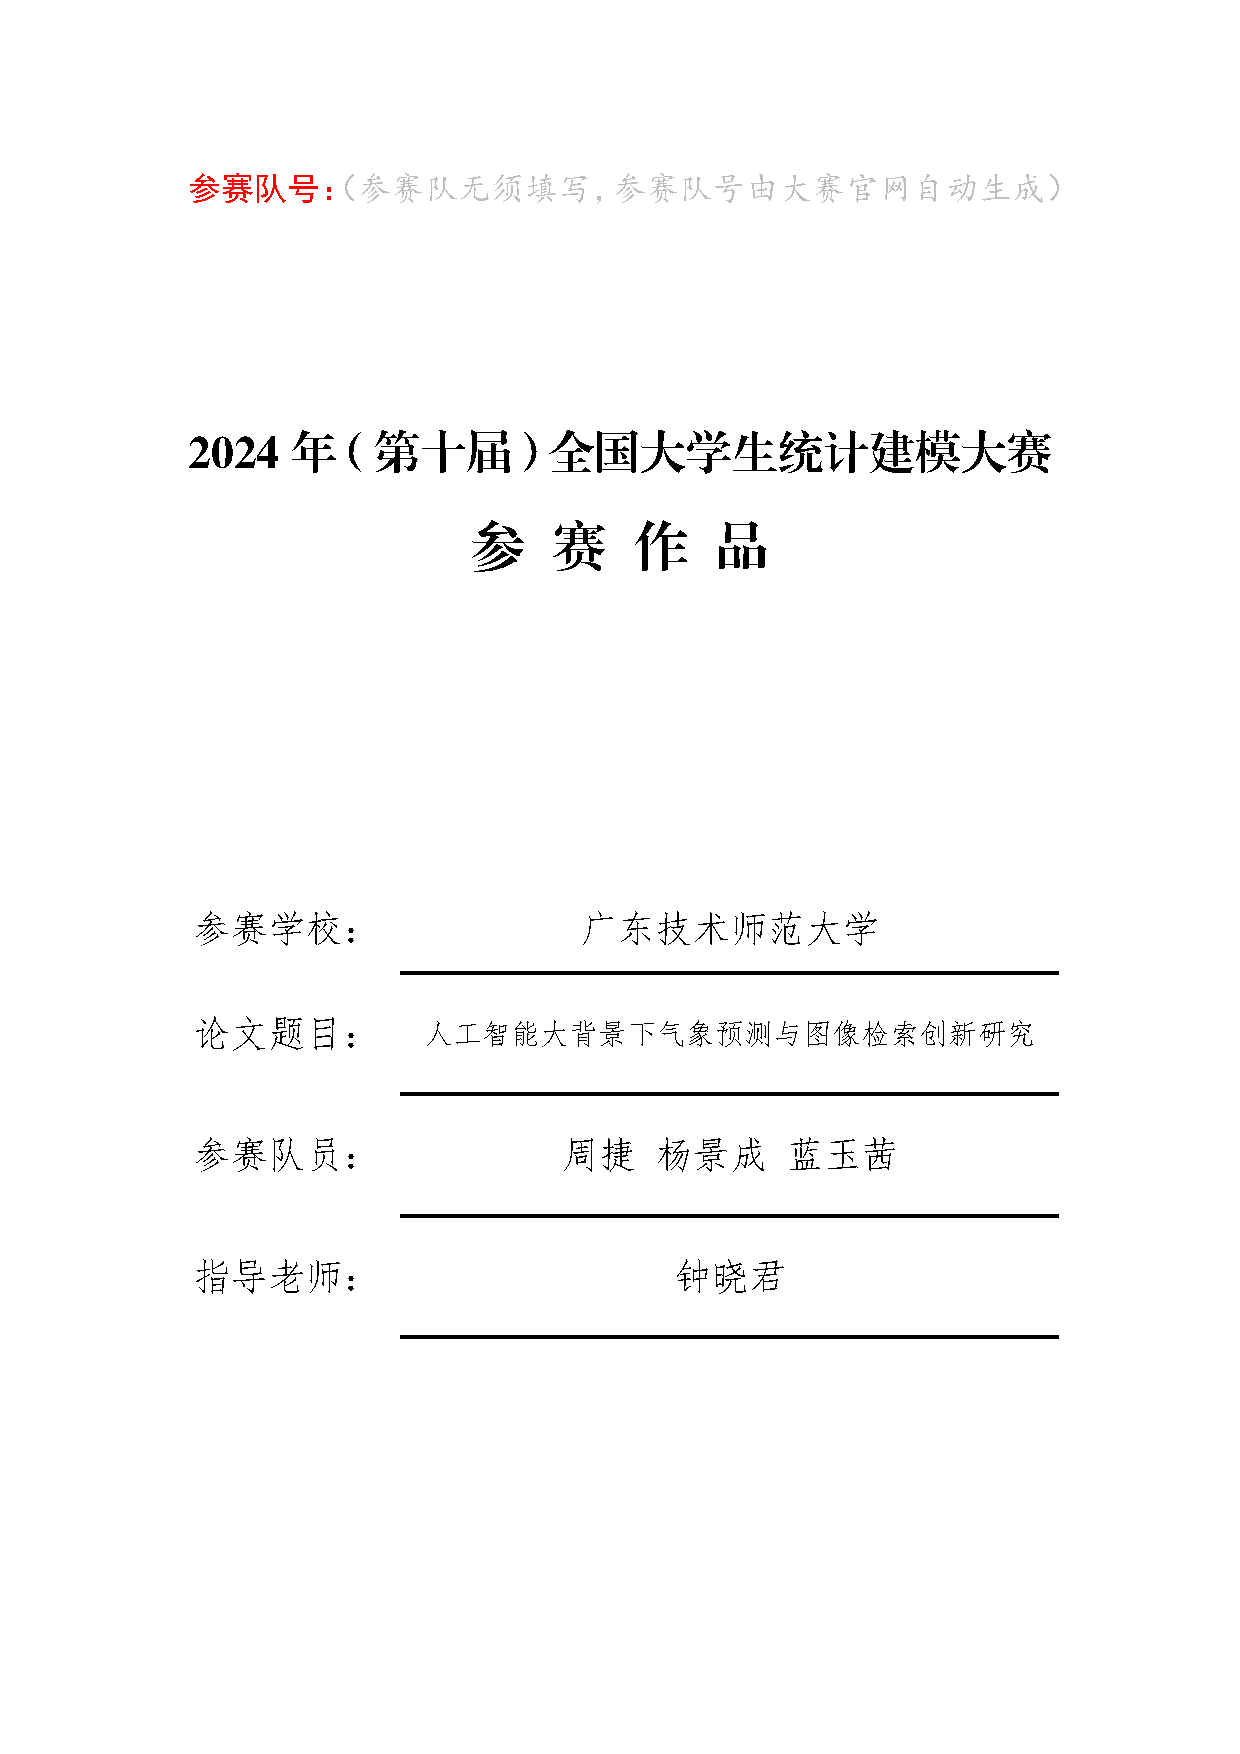
\includepdf[pages={1}]{./documents/title page/封面页.pdf}


%-------------------------摘要部分 起-------------------------
\begin{titlepage}
    \makeabstractstartcn
    \begin{cnabstract}

% 随着互联网技术的飞速发展以及人工智能与大数据技术的不断创新,中国在全球人工智能(AI)和大数据技术应用领域取得了显著进展,并确立了其领先地位。本研究聚焦于这些前沿技术在气象预测和细粒度图像检索领域的创新应用,采用了长短时记忆网络(LSTM)、卷积神经网络(CNN)与LSTM的混合模型(CNN-LSTM),以及细粒度哈希图像检索模型(LGESD),并运用Python编程语言进行全面的数据处理、模型构建、训练和预测。

% LSTM模型首先被应用于时间序列分析,尤其在气象预测方面展现出其卓越的性能。通过融合时间序列分析、机器学习模型和深度神经网络,本研究旨在提升气象预测的精确性、模型的鲁棒性,并优化资源调度效率。进一步地,CNN-LSTM混合模型的提出,通过将时间序列数据图像化,显著增强了特征提取能力,从而进一步提升了气象时间序列预测的准确性。在气象数据集上,经过500个Epoch训练的CNN-LSTM模型,达到了5.0165°C²的均方误差(MSE),有效捕捉了日平均气温的变化趋势。同时,LGESD模型在细粒度图像检索任务中通过显式空间衰减注意机制(ESD)优化特征表达,提升了检索的精确度和效率。在四个公开数据集上的实验结果显示,当哈希码长度为48位时,LGESD模型的平均预测精度(mAP)最高达到了85.06\%,超越了现有技术水平。

% 在模型评估方面,LSTM模型和CNN-LSTM混合模型在气象预测任务中展现了出色的性能,通过训练损失和验证损失的监测,证实了模型的有效性。LGESD模型在图像检索任务中也表现出色,其mAP在多个数据集上均优于现有方法。

% 本研究的优势在于模型对海量数据的适应性强、可扩展性和泛化能力突出、框架设计创新、以及模型评估全面。然而,模型的性能在很大程度上依赖于训练数据的质量和完整性,且在计算资源需求上较高,其泛化能力的进一步验证亦是未来工作的重点。未来的研究可在本研究基础上进行模型改进,以提高预测精度和检索性能。

% 综上所述,本研究成功地将人工智能与大数据技术应用于气象预测和细粒度图像检索领域,推动了技术发展,并为实际应用提供了新方法。研究成果证实,结合LSTM、CNN-LSTM和LGESD模型能够有效提升预测和检索的准确性,为未来的技术进步和应用实践打下了坚实的基础。

% 随着互联网技术的突飞猛进及人工智能与大数据技术的持续突破,国内外在全球AI和大数据应用领域均取得了显著成就。本研究专注于将这些先进技术应用于气象预测与细粒度图像检索,采用了长短时记忆网络(LSTM)、{卷积神经网络(CNN)}与LSTM结合的混合模型(CNN-LSTM),以及细粒度哈希图像检索模型(LGESD),并利用Visual Code、Pycharm、Origin Pro、SpassPro、Excel、WPS进行数据处理、框架图绘制、模型构建、数据分析、训练和预测等等。

% LSTM网络在时间序列分析,尤其是在气象预测方面,展现了其强大的性能。本研究通过整合时间序列分析、机器学习模型和深度神经网络,旨在提高气象预测的精确性与模型鲁棒性,优化资源调度。CNN-LSTM混合模型通过图像化时间序列数据,显著提升了特征提取能力,在实际的测试当中达到了$5.0165 {}^{\circ}\text{C}{}^2$的均方误差(MSE),有效预测了日平均气温变化。LGESD模型通过显式空间衰减注意机制(ESD),在细粒度图像检索任务中提升了检索精确度和效率,其在四个数据集上的平均预测精度(mAP)在哈希码长度为48位时最高达到85.06\%,超越了现有较为先进的方法。


% 在模型评估环节,纯LSTM网络和CNN-LSTM模型在气象预测领域展现了显著的预测能力,这一点通过模型训练和验证过程中损失函数的持续降低得到了证实。LGESD模型在图像检索任务中的表现同样令人瞩目,其在多个数据集上的平均预测精度(mAP)均超越了当前的技术水平。本研究的优势在于模型所表现出的对海量数据的卓越适应性、显著的可扩展性和泛化能力、创新性的框架设计以及全面细致的模型评估过程。然而,我们也注意到模型的性能在很大程度上依赖于训练数据的质量和完整性,同时对计算资源的需求量较大。针对这些挑战,未来的研究工作将着重于进一步验证和提升模型的泛化能力,同时探索模型改进的可能性,以期达到更高的预测精度和图像检索性能。

% 综合实验结果分析,本研究成功地将人工智能与大数据技术融合应用于气象预测和细粒度图像检索领域,不仅推动了相关技术的发展,更为这些领域的实际应用提供了创新的方法。研究成果证明,LSTM网络、CNN-LSTM模型和LGESD模型在分别在各自的领域均能表现出一定的性能,为未来的技术创新和应用实践奠定了坚实的基础。

随着互联网技术的突飞猛进及人工智能与大数据技术的持续突破,国内外在全球AI和大数据应用领域均取得了显著成就。本研究专注于将这些先进技术应用于气象预测与细粒度图像检索,采用了长短时记忆网络(LSTM)、卷积神经网络(CNN)与LSTM结合的混合模型(CNN-LSTM),以及细粒度哈希图像检索模型(LGESD),并利用Visual Code、Pycharm、Origin Pro、SpassPro、Excel、WPS进行数据处理、框架图绘制、模型训练和预测等等操作。

LSTM网络通过融合时间序列分析、机器学习与深度学习技术,在气象预测中提高了预测精度和模型鲁棒性,同时优化了资源调度。新型混合模型 CNN-LSTM 通过图像化时间序列数据,增强特征提取,实测均方误差(MSE)达$5.0165 {}^{\circ}\text{C}{}^2$,有效预测日平均气温变化。LGESD模型创新型地引入了显式空间衰减注意机制(ESD),在细粒度图像检索任务中提升检索精度和效率,四个数据集上平均预测精度(mAP)在哈希码长度48位时最高85.06\%,超越了现有较为先进的方法。

在气象预测领域,纯LSTM网络和CNN-LSTM模型通过持续降低损失函数验证了其显著的预测能力。LGESD模型在图像检索任务中也展现了超越当前技术水平的平均预测精度(mAP)。本研究优势在于模型对大数据的适应性、可扩展性、泛化能力、创新框架设计和细致的评估过程。然而,我们也注意到模型的性能在很大程度上依赖于训练数据的质量和完整性,同时对计算资源的需求量较大。针对这些挑战,未来的研究工作将着重于进一步验证和提升模型的泛化能力,同时探索模型改进的可能性,以期达到更高的预测精度和图像检索性能。

综合实验结果分析,本研究成功地将人工智能与大数据技术融合应用于气象预测和细粒度图像检索领域,不仅推动了相关技术的发展,更为这些领域的实际应用提供了创新的方法。研究成果证明,LSTM网络、CNN-LSTM模型和LGESD模型在分别在各自的领域均能表现出一定的性能,为未来的技术创新和应用实践奠定了坚实的基础。



    \begin{keywordcn}
    人工智能;气象预测;图像检索;CNN-LSTM模型;LGESD框架
    \end{keywordcn}
    
    \addabstractcontentcn
    \end{cnabstract}
\end{titlepage}



\begin{titlepage}
    \makeabstractstarten
    \begin{enabstract}

    As Internet technology advances and AI and big data technologies progress, notable global accomplishments have been made. This study concentrates on applying cutting-edge technologies to weather forecasting and fine-grained image retrieval, using LSTM, CNN-LSTM hybrid models, and LGESD. Tools including Visual Code, PyCharm, Origin Pro, Spasspro, Excel and WPS are employed for tasks from data processing to model development, analysis, training, and prediction.

    LSTM networks enhance weather forecasting by integrating time series analysis, machine learning, and deep learning, improving prediction accuracy and model robustness, and optimizing resource scheduling. The CNN-LSTM hybrid model boosts feature extraction from image-based time series data, achieving an MSE of $5.0165^{\circ}\text{C}^2$ for predicting daily average temperature changes. The LGESD model introduces the explicit spatial decay attention mechanism (ESD) for fine-grained image retrieval, with an average mAP of 85.06\% at a 48-bit hash code length across four datasets, outperforming current advanced methods.

    In weather forecasting, LSTM networks and CNN-LSTM models consistently reduce loss, validating their predictive power. LGESD models also surpass current benchmarks in image retrieval with a mean predictive accuracy (mAP) above state-of-the-art. This study's strengths include the model's adaptability to big data, scalability, generalization, innovative design, and rigorous evaluation. However, model performance is contingent on the quality and completeness of training data and is computationally intensive. Future research will aim to enhance the model's generalization, improve its predictive and retrieval performance, and address these challenges.

    In summary, this study effectively integrated AI and big data in weather prediction and fine-grained image retrieval, advancing the field and offering new practical methods. The findings validate the performance of LSTM networks, CNN-LSTM models, and LGESD models in their respective domains, establishing a strong basis for future technological innovation and application.
    
    \begin{keyworden}
    AI; Weather Forecast; Image Retrieval; CNN-LSTM; LGESD Model
    \end{keyworden}
    
    \addabstractcontenten
    \end{enabstract}
\end{titlepage}




%-------------------------摘要部分 止-------------------------


%-------------------------目录部分 起-------------------------
\makecontent
%-------------------------目录部分 止-------------------------


%=========================正文部分 起=========================

%-------------------------正文开始-------------------------
\maketxtstart
%-------------------------正文开始-------------------------

\section{引言}

\subsection{研究概述}

\subsubsection{研究背景}
1950年,艾伦·图灵提出图灵测试\cite{XSYK202306001},成为评估机器智能水平的重要参照。六年后,“人工智能”一词在美国达特茅斯会议中正式确立,标志着新研究领域的开启。人工智能随时代演进,至今已发展成为一门跨越计算机科学、信息科学、心理学、哲学、认知神经科学及生理学等多个学科的尖端交叉学科 \cite{YUAN200905001},尤其体现在大规模预训练语言模型(又名“基座模型”或“大模型”)的崛起,此类模型凭借庞大的参数规模构建起复杂的神经网络结构\cite{bommasani2022opportunities}。这一技术创新与应用具有里程碑意义,引领研究者跨入通用人工智能研究的新纪元 \cite{ZXTX20240416002}。

\begin{figure}[ht]
  \centering
  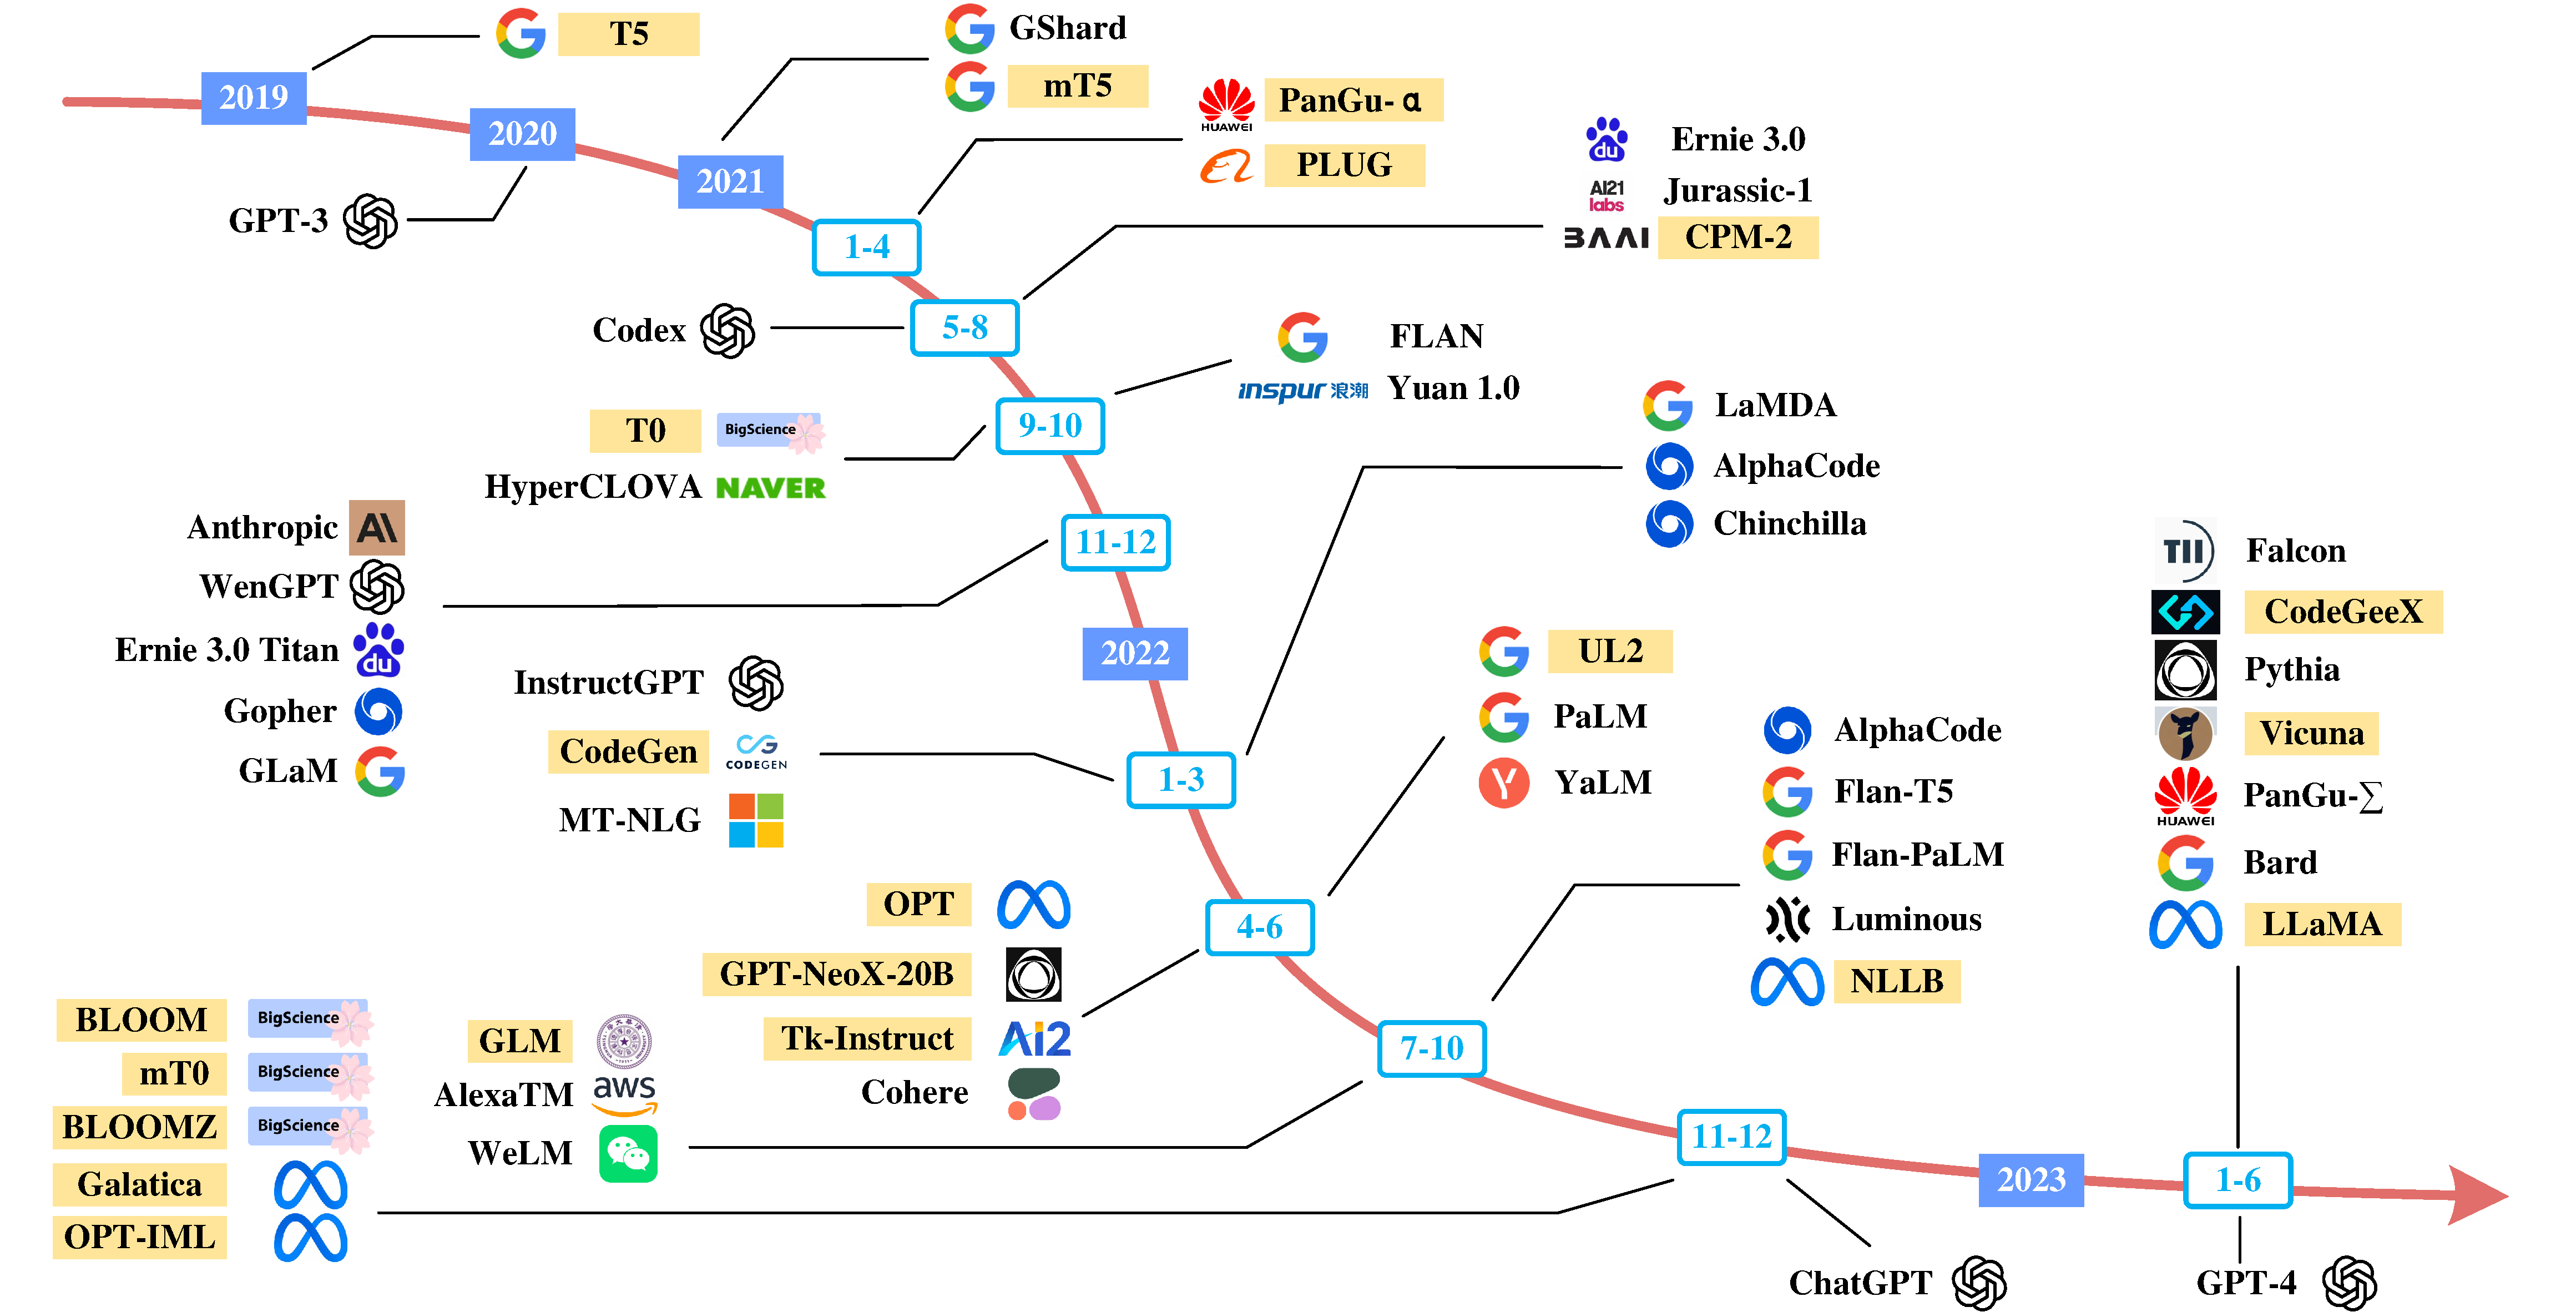
\includegraphics[width=1.0\textwidth]{./Img/大模型发展绘图.pdf}
  \caption{国内外大语言模型整体发展示意}\label{fig:a-00}
\end{figure}

国内外的大模型发展如图 \ref{fig:a-00} 所示,在2020年,OpenAI首次提出的“规模定律”揭示了模型性能随参数规模、数据量及训练持续时间呈指数增长而接近线性提升的趋势,此举显著降低了对传统架构优化及超参数调优的依赖。自此之后,学术与工业界的关注点集中于开发大规模语言模型,其中 GPT-3 \cite{brown2020language} 作为首个达到千亿参数级别的模型,在自然语言处理(NLP)领域实现了多项任务的革新,彰显出前所未有的零样本与少量样本学习效能,为巨型预训练模型时代拉开了序幕。

这一进展进一步激发了科技巨头如谷歌、Meta的竞争,纷纷推出百亿乃至千亿参数量级的模型,例如Gopher、Chinchilla、PALM等,这些模型的参数量达到了数十亿甚至数千亿。在2022年,大模型展现出的卓越性能在全球范围内引发了研发热潮,众多大模型如雨后春笋般涌现,国际上InstructGPT、MT-NLG、OPT、LLaMA-2、Flan、Luminous和ChatGPT \cite{chatgpt2022} 等大模型相继发布。与此同时,国内也推出了GLM-130B、ChatGLM2、WeLM、PanGu等重要的大模型。这些模型的发布进一步丰富了大模型生态系统,使其显得更加充满活力。

\begin{figure}[h]
  \centering
  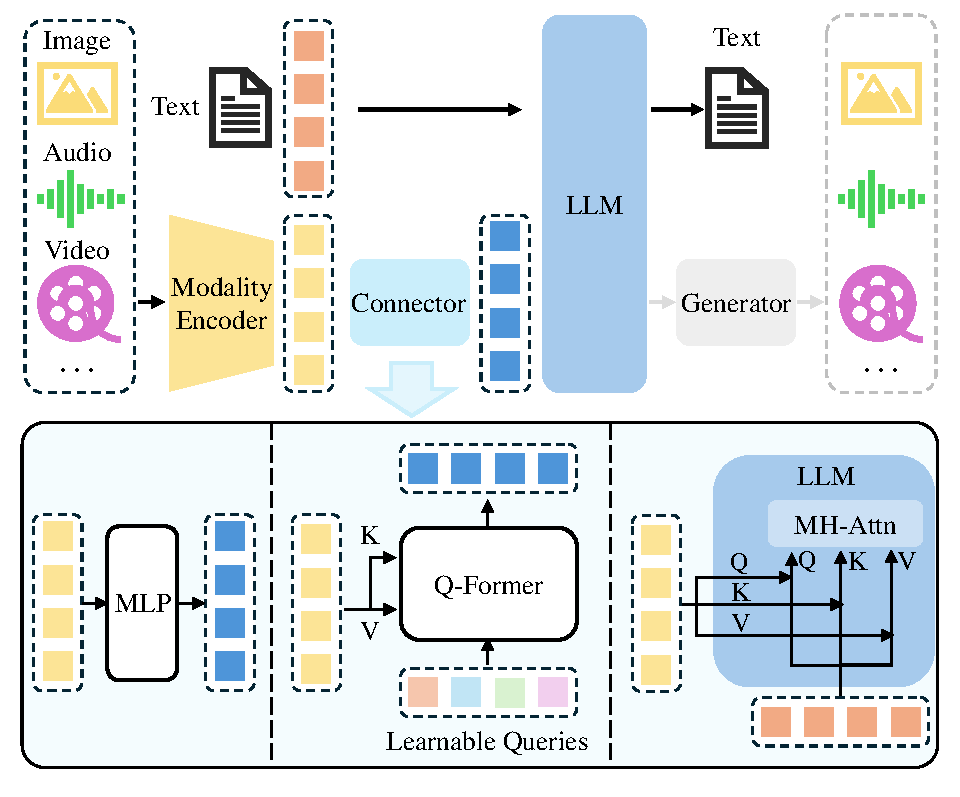
\includegraphics[width=0.8\textwidth]{./Img/多模态大模型结构.pdf}
  \caption{多模态大模型结构}\label{fig:a-01}
\end{figure}


\begin{figure}[ht]
  \centering
  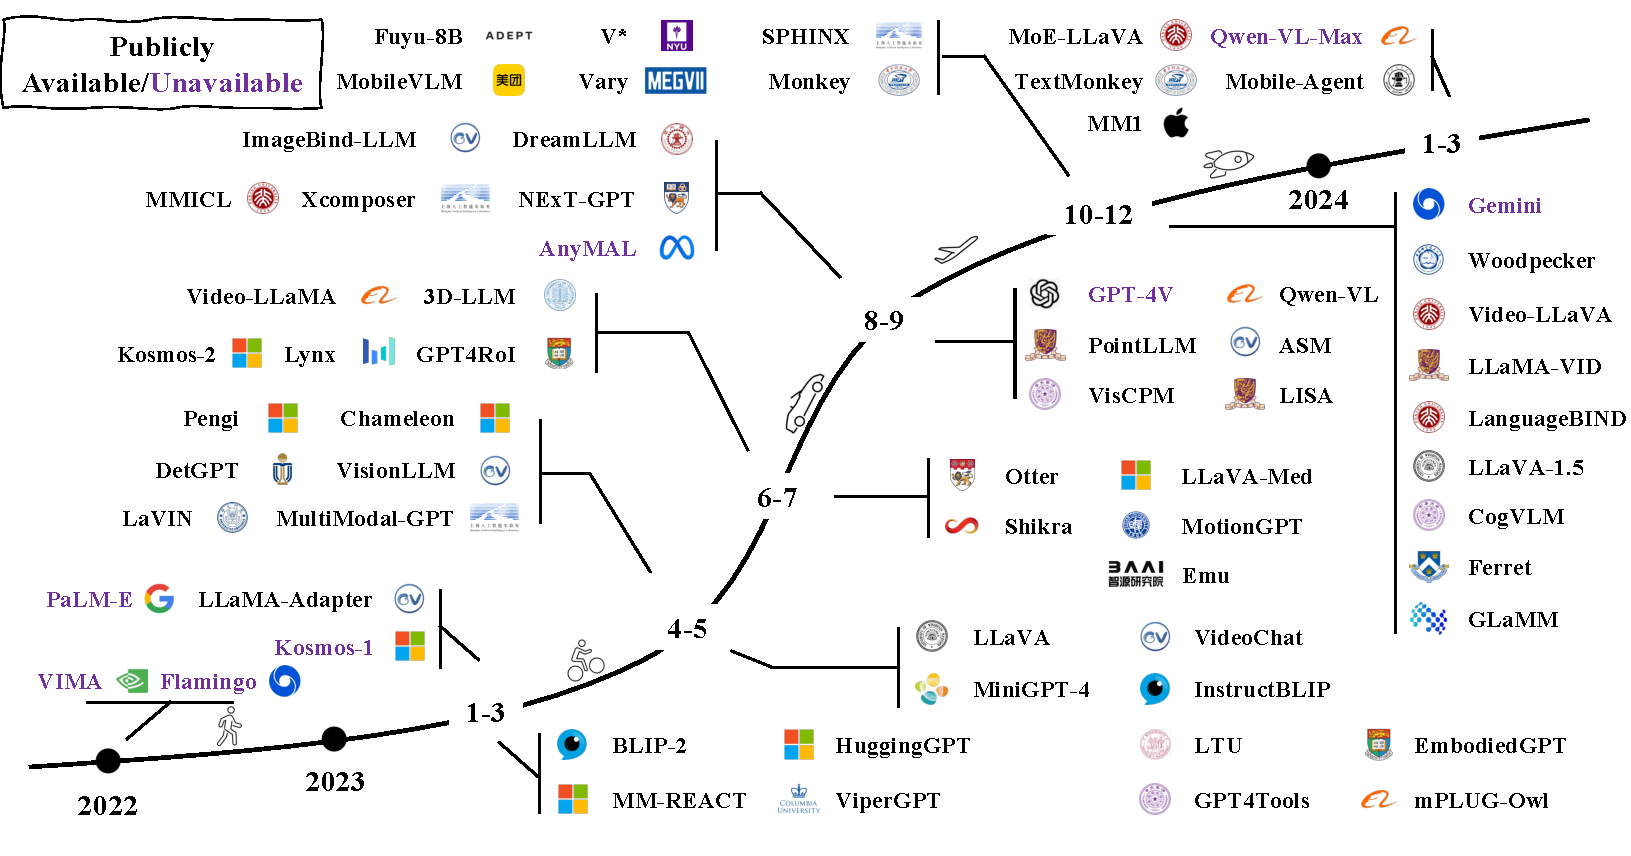
\includegraphics[width=1.0\textwidth]{./Img/多模态大语言模型.pdf}
  \caption{国内外多模态大语言模型发展示意}\label{fig:a-02}
\end{figure}


在图 \ref{fig:a-00} 展示的大语言模型宏观格局中,一个突出的现象是大多数模型集中在单一模态任务上,即文本到文本的生成。然而,自2022年以来,一种新型的多模态大语言模型(MLLM)开始崭露头角,它们能够跨越文本、图像和视频这三种不同模态的界限,实现不同模态间的自由生成。这些多模态大型模型的普遍的内部结构如图 \ref{fig:a-01} 所示\cite{yin2024survey},它包括一个编码器(Encoder)、一个连接器(Connector)和一个大语言模型(LLM)。 大语言模型可以附加一个可选的生成器,以生成除文本之外的更多模式。 编码器接收图像、音频或视频并输出特征,这些特征由连接器处理,以便大语言模型可以更好地理解。 其中连接器大致分为三种类型:基于投影的连接器、基于查询的连接器和基于融合的连接器。 前两种类型采用令牌级融合,将特征处理成令牌与文本令牌一起发送,而最后一种类型则在大语言模型内部实现特征级融合。

在这类框架的基础上,多模态大语言模型引发了一场前所未有的研发热潮,在图 \ref{fig:a-02} 中,我们可以看到多模态大语言模型(MLLM)的发展历程。黑色和蓝色的线条分别代表开源和闭源模型,清晰地展示了它们在时间轴上的进展。2022年标志着多模态大语言模型的诞生,其中 VIMA 和 Flamingo 作为该领域的先驱模型,为后续的发展奠定了基础。然而,对于多模态大语言模型(MLLM)而言,真正的转折点出现在2023年,在这一年,我们目睹了一场前所未有的技术革新浪潮,多模态大语言模型的发展呈现出爆炸性的增长。全球科技巨头们在这一年里竞相推出了他们的创新模型,如谷歌(Google)、Meta、微软(Microsoft)、阿里巴巴(Alibaba)、OpenAI,以及苹果(Apple)等领先科技公司纷纷展示了他们在MLLM领域的最新研究成果。

除了工业界之外,学术界同样展现出了强劲的竞争力和创新精神。2023年,不仅是科技公司的丰收年,也是学术界的重要里程碑。新加坡国立大学、南洋理工大学、清华大学、北京大学、香港大学、复旦大学以及上海交通大学等全球顶尖高等学府的师生们在这一年中,通过他们的智慧和努力,为多模态语言理解技术的理论和应用实践做出了显著贡献。这些学府的研究成果,无论是在深化理论研究,还是在推动技术应用方面,都极大地拓展了MLLM的边界。他们的工作不仅加速了学术交流,也为工业界提供了宝贵的知识和技术支持,促进了整个领域的健康发展。图 \ref{fig:a-02} 以其详尽的时间线和关键的模型发展节点,绘制出了2023年多模态大语言模型的蓬勃发展图景。这一年,MLLM的发展达到了一个新的高潮,成为了全球科技竞争和合作的一个缩影。它不仅标志着多模态语言理解技术的一个关键转折点,更预示着人工智能技术未来发展的方向和趋势。

随着人工智能技术的突飞猛进,尤其是多模态大型语言模型(MLLM)的应用,我们在处理复杂任务方面的能力得到了显著提升。这些模型通过先进的文本生成技术,即自然语言处理(NLP)的核心,不断推动着智能系统的边界。在这样的技术浪潮推动下,我们本次的研究专注于探讨人工智能大背景下的两个领域出发:

\begin{itemize}[leftmargin=3em]
    \item \textbf{大数据技术}:驱动气象预测的精准化转型与效能优化。
    \item \textbf{人工智能技术}:基于计算机视觉图像检索图像的的深化研究与应用实践。
\end{itemize}

通过人工智能与数据科学的紧密融合,为气象预测及大规模细粒度图像检索领域带来了前所未有的革新动力与广阔前景,显著增强了这些领域的预测精度与检索效率。

\subsubsection{研究意义}

在大模型技术的强力驱动下,研究领域迅速拓展,深入涉及深度学习、机器学习、智慧教育、个性化学习、自适应学习、情感计算、学习分析以及教育大数据等多个尖端且关键的主题领域。鉴于此,本研究计划专注于人工智能在气象预测优化及大规模图像处理的双重应用领域,旨在通过深化AI技术的研究与创新实践,提升气象预测的精确性以及模型的鲁棒性,并优化资源调度的效率。同时,针对大规模图像数据处理中对于高精度识别与分析的迫切需求,尤其是在细粒度图像检索、人脸识别、目标检测及语义分割等关键技术环节,我们将积极探究并推广人工智能算法的高效应用途径,进一步拓宽人工智能技术在气象预测分析及大规模图像智能处理领域的应用边界与发展潜力。

\textbf{气象预测}是气象学、应急管理和多个依赖气候条件行业的核心关注点,它运用统计学、机器学习、人工智能等技术手段,旨在预测特定地区未来一段时间内的天气状况,包括温度、降水、风力等关键指标,对农业规划、能源分配、交通运输及公众安全等领域具有重要指导意义。在气象预测领域 \cite{HJKZ2024011600J},我们融合了大数据与深度学习的最新研究成果,运用历史气象数据挖掘气候模式,旨在揭示天气变化的内在规律,并实现对气象变量多维度的精密解析。通过融合时间序列分析、灵活的机器学习模型及深层神经网络,我们能够快速适应天气系统变化,实时监控气象,准确预测极端事件,优化调度策略,为气象服务、灾害预警及保障公共安全提供智能辅助决策,提升气象预测的准确率与应变效率。

\textbf{大规模细粒度图像检索}(Large-scale Fine-grained Image Retrieval)是一种专注于在庞大图像数据库中,精准查找具有细微差异的同类物品图像的技术。与一般的图像检索不同,细粒度检索关注的是那些属于同一类别但存在微小差异的对象,比如不同种类的鸟类、植物、汽车型号或服装款式等。在图像检索领域,深度学习和多模态大模型的发展,极大地提升了图像识别和分类的准确性。这些技术在处理大规模图像数据集时,能够通过学习细粒度特征,实现高效、精确的图像匹配和检索。例如,通过结合卷积神经网络(CNN)\cite{LeCun2015}和Transformer \cite{vaswani2023attention} 的架构,可以对图像进行深度分析,提炼出高度抽象且富有代表性的特征,提高检索的准确性和泛化能力。

\subsection{研究现状与方法}

\subsubsection{研究现状}

在\textbf{气象预测}这一研究领域,马飞等(2024)\cite{JYGC20240415002} 提出一种融合气象和交通特征数据的GAF-CNN-LSTM短时交通流预测方法,通过将时间序列数据转换为图像并利用深度学习提取特征,显著提升了预测精度。沈金星等(2024)\cite{HJKZ2024011600J} 结合了CNN、LSTM以及注意力机制三个模块,有效捕捉了气象特征的时序非线性变化,显著优于对比模型。马国斌等(2011)\cite{ZHXU201103002} 基于自然灾害风险理论,利用GIS空间分析功能和归一化及层次分析法,对中国进行了洪涝灾害危险性评估,开发了一个全国洪涝灾害危险性评估模型,并以此为基础生成预警产品,为防灾减灾提供决策支持。陈聪等(2023)\cite{1023751652ch} 针对暴雨灾害,提出了集成经验模态分解-马尔科夫(D-Markov)模型;同时针对大气污染问题,设计了基于卷积门控循环单元(CNN-GRU)的预测系统。通过实验验证,这两种模型都能提供高精度的预测结果,为防灾减灾提供了有力支持。屈峰等(2024)\cite{HBYD202401011} 提出一种结合小波分析、LSTM网络和卡尔曼滤波技术的混合方法,有效预测短期风速变化趋势,并通过实证分析验证了其预测性能。申洪涛等(2024)\cite{DLJS202401002} 提出一种结合小波分析、LSTM网络和卡尔曼滤波技术的混合方法,有效预测短期风速变化趋势,并通过实证分析验证了其预测性能。Charlton-Perez 等(2024)\cite{charltonperez2024ai} 通过分析机器学习模型对高影响天气事件——风暴Ciarán的预测表现,揭示了这些模型在模拟宏观天气结构方面的准确性,但在细节捕捉上存在局限,指出了机器学习在天气预测精度提升上需要进一步研究的必要性。


\textbf{细粒度图像检索}源自于人工智能领域中细粒度图像分析方面\cite{wei2021finegrained}的一个基本主题,近年越来越受到重视\cite{solving9157668}\cite{cui2020exchnet}\cite{zheng2019towards}。依据查询图像的本质特性,细粒度图像检索任务可被区分为两大类别:一是基于内容的细粒度图像检索(FG-CBIR),二是基于草图的细粒度图像检索(FG-SBIR)。具体地,早期在FG-CBIR领域中,研究工作如 SCDA \cite{wei2017selective} 引入了深度预训练网络的应用,而这一过程并不依赖于明确的局部化监督信息。随后,为了解决无监督检索在准确率上的局限性,一系列基于监督的度量学习策略应运而生 \cite{HoIH8237325},旨在通过引入额外的指导信号来优化检索性能。

在另一研究轨迹上,基于手绘草图的图像检索(FG-SBIR)作为一个引人注目的领域,专注于将手绘草图作为查询工具,以便精确地从现实照片中找到对应物体。这一领域是细粒度图像检索与跨模态检索交汇的核心。现有技术,如文献\cite{Yu7780462SMTS}\cite{song8237854DSA}所展示,关键在于构建一个嵌入空间,使得草图和照片可以在此空间中通过最近邻搜索高效匹配。尽管当前的细粒度图像检索方法通常依赖深度网络的最终特征层输出来进行检索,并在一些场合取得了显著效果,但面对大规模数据集时,这些方法的局限性显而易见。特别是在大规模图像检索任务中,要实时找到与查询最匹配的精确最近邻,常常面临巨大的时间成本挑战,有时在实际执行中几乎不可行。

面对这一挑战,细粒度哈希技术应时而生,被视为一个极具潜力的解决方案。该技术旨在生成紧凑的二进制编码,以高效地捕捉和表征细粒度对象的独有属性,因此近年来在细粒度图像检索的研究界获得了广泛关注 \cite{solving9157668}\cite{Zeng_2024}\cite{DSH9037360}。

\subsubsection{研究方法}

\textbf{数据处理的创新}:
在气象预测研究中,我们采用前向填充策略处理缺失值,即用时间序列的均值填补,同时排除了缺失三个及以上指标的记录以保证数据质量。所有数据在模型训练前都经过归一化,以统一数据范围,优化模型学习效率和预测准确性。在图像检索研究中,鉴于图像尺寸参差不齐,我们针对每一张图像放大为 $256 \times 256$,然后针对训练图像和测试图像分别采用随机裁剪为$224 \times 224$和中心裁剪为 $224 \times 224$ 两种方式,最后按照国际公认的标准进行归一化,最后得到标准的RGB三通道的图像数据,确保评估模型时所使用图像数据的公平性。

\textbf{气象预测技术的创新}:在气象预测领域,长短期记忆网络(LSTM)因其在处理时间序列数据方面的独特优势而备受青睐。LSTM网络通过其精巧的门控机制,能够有效捕捉时间序列中的长期依赖关系,这对于模拟气象现象中复杂的动态变化至关重要。鉴于气象变化的精细时间关联和不可预测性,LSTM在揭示气象数据内在规律方面展现出了卓越的能力。此外,LSTM模型与卷积神经网络(CNN)、小波分析以及多种优化算法的结合使用\cite{HJKZ2024011600J}\cite{JYGC20240415002}\cite{HBYD202401011}\cite{DLJS202401002},进一步扩展了其在气象预测研究中的应用潜力。受混合网络模型的启发,我们设计了一个结合了卷积神经网络(CNN)和长短时记忆网络(LSTM)互补优势的混合模型。在模型训练阶段,我们通过特征工程精心筛选了对预测任务至关重要的特征,并通过对学习率、批量大小和迭代次数等超参数的精细调整,优化了模型的性能。在评估过程中,我们采用了均方误差(MSE)和平均绝对百分比误差(MAPE)等指标来量化模型的预测效能,以确保我们的混合模型能够在气象预测任务中提供高精度的预测结果。

\textbf{图像检索技术的创新}:在图像检索的研究领域,我们提出了一种创新的细粒度哈希检索框架,命名为LGESD(Local and Global learning of Explicit Spatial Decay)。该框架的设计精髓在于其独特的双层结构,这一结构融合了全局哈希映射单元与局部哈希映射单元,旨在生成能够同时捕获图像全局语义信息和局部细节信息的二进制哈希码。这种设计显著提升了哈希码的表达能力和图像检索任务中的区分度。同时,在注意力机制的改进上,LGESD框架创新性的设计了显式空间衰减注意机制(ESD),这一机制在生成全局和局部特征时,通过考虑特征之间的空间关联性和衰减特性,确保了特征的互补性并增强了特征的唯一性。这种显式建模特征间的空间关系的方法,为图像检索任务提供了更为丰富和鲁棒的特征表示。在一系列实验中,我们展示了LGESD框架在多个标准图像数据集上的性能,验证了其在图像检索任务中的准确性和泛化能力。实验结果表明,LGESD框架在处理细粒度图像检索任务时,相较于现有技术,展现出了显著的性能优势。


% \begin{equation}
%   \int_0^{+\infty}\frac{x}{\mathrm{e}^x-1}\mathrm{d}x=\frac{\pi^2}{6}
% \end{equation}



\section{指标选取与数据说明}

\subsection{指标的选取}

在气象预测的研究的中,本文精选了一组关键气象指标,如日均温度、日最高温度、日最低温度、降水量、相对湿度和风速,以全面捕捉气象数据的复杂性。此外,为了增强数据集的深度,我们引入了平均气压这一参数,它为模型提供了额外的信息维度,并在CNN-LSTM模型中证明了其有效性。

在对细粒度哈希图像检索模型进行研究的过程中,我们选定了鸟类、食物类、飞机类以及北美鸟类等多样化的类别作为评估标准。这些精心挑选的指标不仅彰显了本研究的广度和深度,同时也为与现有方法的比较提供了一个公平的基准。借助这些指标,我们得以更精确地评估模型的性能,进而为图像识别领域带来了新的研究视角和分析维度。

\subsection{数据汇总及来源说明}

在本项研究中,我们利用了一套综合性且广泛涵盖的数据资源,确保了该研究在气象学领域以及众多计算机视觉子领域中保持了一定程度的公正性。

\textbf{气象数据}:为确保气象数据分析的可靠性和准确性,我们严谨地采用了国家气象信息中心提供的高标准基础数据。数据集一涵盖了2015年2月至2016年8月这一时段,精心选取了日均温、日最高温、日最低温、相对湿度及风速等关键参数;而数据集二则聚焦于2013年1月至2017年4月,除了包含日均温、相对湿度与风速外,还加入了平均气压指标,以此构建起更为全面多元的气象数据体系。

\textbf{图像数据}:为了进一步丰富研究内容的多样性,并将研究范围扩展到图像识别的尖端领域,我们融合了多个国际公认的公开数据集,经过实验分析之后,我们选取了国际公开数据中的4个不同领域的数据集,具体细节如下所述:
\begin{itemize}[leftmargin=2em]
    \item CUB200-2011数据集:专注于鸟类图像分类,包含200个不同的鸟种,为生物多样性研究提供了丰富的视觉资源;
    \item Food101数据集:集合了101种食物的大量图像,适用于食品识别技术的开发与评估;
    \item Aircraft数据集:该数据集专为飞机识别而设计,收集了全球范围内100种不同型号的飞机图像,在复杂目标识别中具有重要的研究价值;
    \item NABirds数据集:这个数据集包含555个鸟类品种,均来自北美地区,被用于研究物种识别的地域特异性。
\end{itemize}

这种跨域数据集的集成为图像分析算法带来了新挑战,考验模型的泛化能力,在未知的数据上仍能保持高效准确的识别性能,同时也要求模型能够学习到跨数据集通用的特征表示,并且能够捕捉到各个数据集之间共有的以及独特的视觉模式。通过这样的挑战,研究者们被推动去探索更为先进的机器学习技术,包括深度学习、迁移学习、多任务学习、领域自适应等策略,以促进模型对异质数据的适应性和鲁棒性。




\section{研究假设与变量说明}

\subsection{研究假设}

% \begin{itemize}
%     \item 依据与理由:卷积神经网络(CNN)和长短期记忆网络(LSTM)各自在图像识别和时间序列分析方面展现出强大的性能。CNN擅长捕捉空间特征,而LSTM能够处理时间依赖性。假设一:结合CNN和LSTM的混合模型能够通过深度学习技术更全面地捕捉气象数据的非线性特征和长期依赖性,预期将提供超越传统模型的预测精度。
    
%     \item 依据与理由:时间序列数据的可视化是理解其内在结构和模式的重要手段。CNN-LSTM模型结合了时间序列分析与空间特征提取的能力。假设二:CNN-LSTM模型通过将时间序列数据可视化,能够识别并解析气象数据的复杂结构,从而增强模型的预测能力。
    
%     \item 依据与理由:在大数据时代,处理大规模数据集的效率和准确性是模型成功的关键。LSTM因其独特的记忆机制,适合处理序列数据,而CNN能够高效处理图像数据。假设三:在大数据环境下,LSTM和CNN-LSTM模型将展示出对大规模气象数据集的高效处理能力,确保预测的速度和准确性。
    
%     \item 依据与理由:LGESD模型作为一种细粒度哈希检索框架,已在图像检索任务中显示出高效的性能。假设四:LGESD模型将维持其在大规模图像检索任务中的高效性能,即便面对数据量的显著增加。


% \end{itemize}
\subsubsection{卷积神经网络(CNN)与长短期记忆网络(LSTM)的结合}

卷积神经网络(CNN)在图像识别任务中表现出卓越的性能,主要归功于其强大的空间特征捕捉能力。与此同时,长短期记忆网络(LSTM)在处理时间序列数据方面同样表现出色,这得益于其对时间依赖性的敏感性。基于这两种网络的优势,我们提出以下假设:

\textbf{假设一}: 结合CNN和LSTM的混合模型能够通过深度学习技术更全面地捕捉气象数据的非线性特征和长期依赖性,预期将提供超越传统模型的预测精度。

\subsubsection{时间序列数据的可视化与模型预测能力}

时间序列数据的可视化是理解其内在结构和模式的重要手段。CNN-LSTM模型结合了时间序列分析与空间特征提取的能力,这可能对模型的预测能力产生显著影响。因此,我们提出第二个假设:

\textbf{假设二}: CNN-LSTM模型通过将时间序列数据可视化,能够识别并解析气象数据的复杂结构,从而增强模型的预测能力。

\subsubsection{大规模数据处理与模型效率}

在大数据时代背景下,模型处理大规模数据集的效率和准确性至关重要。LSTM因其独特的记忆机制,适合处理序列数据,而CNN能够高效处理图像数据。这引导我们提出第三个假设:

\textbf{假设三}: 在大数据环境下,LSTM和CNN-LSTM模型将展示出对大规模气象数据集的高效处理能力,确保预测的速度和准确性。

\subsubsection{图像检索任务中的LGESD模型}

LGESD模型作为一种细粒度哈希检索框架,在图像检索任务中已显示出高效的性能。考虑到其在大规模图像检索任务中的潜力,我们提出最后一个假设:

\textbf{假设四}: LGESD模型将维持其在大规模图像检索任务中的高效性能,即便面对数据量的显著增加。

\subsection{变量说明}

在本研究中,所涉及到的符号和参数的相关定义如下表 \ref{tab:parameter_explain} 所示:

\begin{table}[h]
    \caption{符号和参数的相关定义}\label{tab:parameter_explain}
    \centering
    \resizebox{0.9\linewidth}{!}
    {\begin{tabular}{*4{c}}
    \toprule
    符号定义 & 符号说明 & 符号定义 & 符号说明 \\
    \midrule
        $t$       & 时间步索引                       & $I$           & 输入图像             \\
        $h_{t-1}$  & 上一个时间步的隐藏状态            & $T$           & CNN提取的深度激活张量     \\
        $x_t$     & 当前时间步的输入                  & $\widehat{T}$& 全局特征的映射          \\
        $W_f, W_i, W_o$ & 遗忘/输入/输出门权重矩阵     & $\widehat{T}_i^{\prime}$ & 局部特征的映射      \\
        $b_f, b_i, b_o$ & 遗忘/输入/输出门偏置项       & $Q$         & 注意力机制中的查询        \\
        $\sigma$  & Sigmoid激活函数                  & $K$         & 注意力机制中的键         \\
        $\tanh$   & Tanh激活函数                     & $V$         & 注意力机制中的值         \\
        $C_{t-1}$  & 上一个时间步的Cell状态            &   $u$       &        二进制哈希码         \\ 
        $\tilde{C}_t$ & Tanh激活后的候选Cell状态       & $D_{2d}$    & 二维空间衰减矩阵         \\
        $C_t$     & 当前时间步的Cell状态               & $\gamma$    & 空间衰减注意力中的超参数     \\
        $o_t$     & 当前时间步的输出门激活值             & $x_n$       & 第n个元素的空间位置横坐标    \\
        $f_t^*$   & 遗忘门的带权输入                   & $x_m$       & 第m个元素的空间位置横坐标    \\
        $i_t^*$   & 输入门的带权输入                   & $y_n$       & 第n个元素的空间位置纵坐标    \\
        $h_t$     & Cell输出的激活函数                 & $y_m$       & 第m个元素的空间位置纵坐标   \\
    \bottomrule
    \end{tabular}}    
    \vspace{-0.8em}
\end{table}

        % 1    & 当前时间步的输出门激活值     \\
        % 1    & Tanh激活函数         \\
        % 1    & 遗忘门的带权输入         \\
        % 1    & 输出门的带权输入         \\
        % 1    & 遗忘门的激活值          \\
        % 1    & 输出门的激活值          \\
        % 1    & 当前时间步的Cell状态     \\
        % 1    & Cell输出的激活函数      \\
        % 1    & 输入图像             \\
        % 1    & CNN提取的深度激活张量     \\
        % 1    & 全局特征的映射          \\
        % 1    & 局部特征的映射          \\
        % 1    & 注意力机制中的查询        \\
        % 1    & 注意力机制中的键         \\
        % 1    & 注意力机制中的值         \\
        % 1    & 二维空间衰减矩阵         \\
        % 1    & 空间衰减注意力中的超参      \\
        % 1    & 第n个元素的空间位置横坐标    \\
        % 1    & 第m个元素的空间位置横坐标    \\
        % 1    & 第n个元素的空间位置纵坐标    \\
        % 1    & 第m个元素的空间位置纵坐标   \\


\section{模型构建与分析}

\begin{figure}[ht]
  \centering
  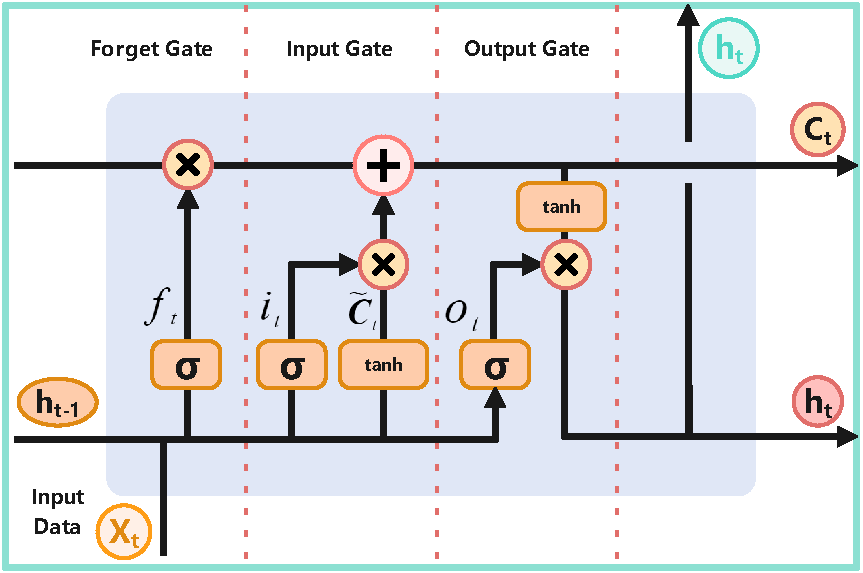
\includegraphics[width=0.65\textwidth]{./Img/LSTM解释结构图.pdf}
  \caption{LSTM详细结构图}\label{fig:a-0}
\end{figure}

\subsection{LSTM长短时记忆网络}
\label{subsec:lstm}

\subsubsection{算法介绍}

LSTM(Long Short-Term Memory Networks,长短时记忆网络),由Hochreiter和Schmidhuber于1997年提出 \cite{LSTM_Hochrerter},目的是解决一般循环神经网络中存在的梯度爆炸(输入信息激活后权重过小)及梯度消失(例如sigmoid、tanh的激活值在输入很大时其梯度趋于零)问题,主要通过引入门和Cell状态的概念来实现梯度的调整。LSTM采用了门控输出的方式,即三门(输入门、遗忘门、输出门)两态(Cell State长时、Hidden State短时)。其核心即Cell State,指用于信息传播的Cell的状态,其结构示意图如图 \ref{fig:a-0}所示。


\subsubsection{数据预处理}

在开展气象预测模型的研究过程中,我们选取了从2015年2月至2016年8月期间的气象记录作为研究样本。此数据集不仅包含了日期基本信息(年、月、日),还涵盖了日均温、日最低温、日最高温、相对湿度、风速和降水量等多个关键气象参数。

\begin{table}[!ht]
    \caption{2015年2月-2016年8月期间的有效气象数据}\label{tab:LSTM_data}
    \centering
    \resizebox{1.0\linewidth}{!}
    {\begin{threeparttable} 
    \begin{tabular}{*9{c}}\toprule
        序号 & 年份 & 月份 & 日号 & 日最高气温\tnote{1} & 日最低气温\tnote{1} & 日平均气温\tnote{1}  & 相对湿度($\%RH$) & 降水量($mm$) \\  
        \midrule
        1 & 2015 & 2 & 1 & 1.9 & -0.4 & 0.7875 & 75.000 & 160.477961 \\ 
        2 & 2015 & 2 & 2 & 6.2 & -3.9 & 1.7625 & 77.250 & 129.268657 \\ 
        3 & 2015 & 2 & 3 & 7.8 & 2.0 & 4.2375 & 72.750 & 107.316539 \\ 
        4 & 2015 & 2 & 4 & 8.5 & -1.2 & 3.0375 & 65.875 & 132.549075 \\ 
        5 & 2015 & 2 & 5 & 7.9 & -3.6 & 1.8625 & 55.375 & 91.082841 \\ 
        $\cdots$ & $\cdots$ & $\cdots$ & $\cdots$ & $\cdots$ & $\cdots$ & $\cdots$ & $\cdots$ & $\cdots$ \\ 
        576 & 2016 & 8 & 29 & 29.9 & 18.1 & 23.7125 & 62.500 & 283.897344 \\ 
        577 & 2016 & 8 & 30 & 29.3 & 16.9 & 23.3250 & 71.500 & 299.212180 \\ 
        578 & 2016 & 8 & 31 & 30.4 & 18.6 & 24.5250 & 68.750 & 292.517916 \\
        \bottomrule
    \end{tabular}    
    \begin{tablenotes}    
        \small              
        \item[1] 气温单位:${}^{\circ}\text{C}$
    \end{tablenotes}          
    \end{threeparttable}}
    \vspace{-0.8em}
\end{table}


在数据预处理阶段,针对数据集中出现的缺失值和异常值,我们选择在该数据集中采取了向前取该时间序列中可用数据的均值进行填补的策略,并剔除了缺失超过三项气象指标的数据,以确保分析的严谨性。经过这一系列处理后,最终得到了共计578条有效气象观测数据,整理后的有效数据如表 \ref{tab:LSTM_data} 所示。



\subsubsection{模型建立}\label{subsubsec:lstm_model_build}

在LSTM中,Memory Cell接受两个输入,即上一时刻的输出值 $h_{t-1}$ 和本时刻的输入值 $X_t$ ,由这两个参数先进入遗忘门,得到决定要舍弃的信息 $f_{t}$ 后,再进入输入门,得到要更新的信息 $i_t$ 和当前时刻的Cell状态 $\widetilde{C}_t$ ,最后由遗忘门与输入门的输出值(即 $f_t$,$X_t$,$\widetilde{C}_t$)进行组合,组合的计算公式如下所示:
\begin{align}
    h_t = C^{t-1} \times f_t \times \widetilde{C}_t \times i_t
\end{align}

其中,$C^{t-1}$表示上一时刻的Cell状态,$f_t$ 为遗忘信息的激活值,$\widetilde{C}_t$ 为当前时刻Cell状态,$i_t$ 表示当前时刻需要记忆信息的激活值,得到分别的长时 $C_t$ 和短时 $h_t$ 信息,最后进行存储操作及对下一个神经元的输入。因此,LSTM在网络中的工作流程如下图所示:


\begin{figure}[ht]
  \centering
  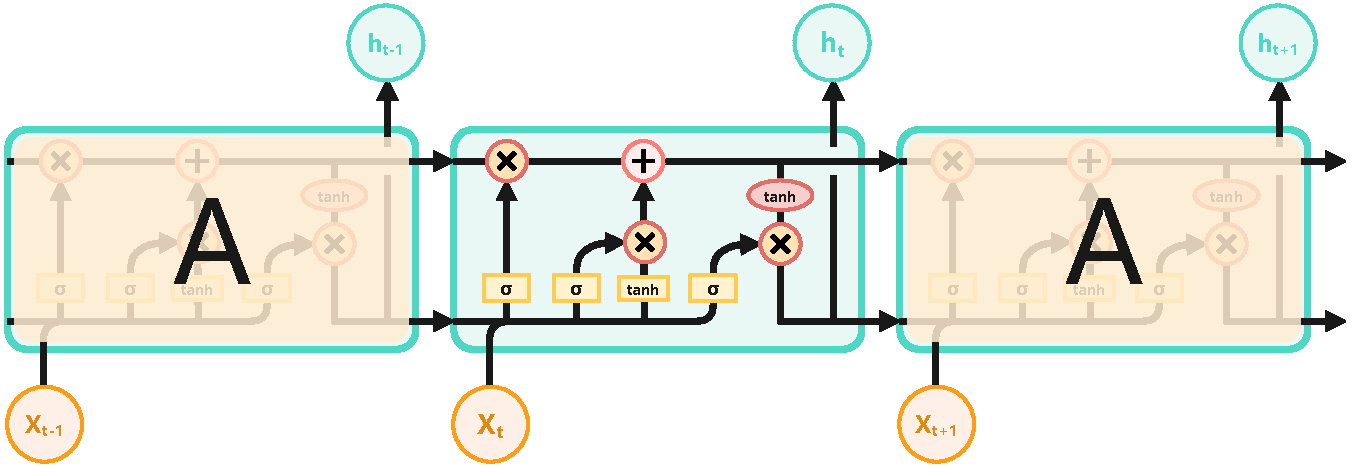
\includegraphics[width=0.9\textwidth]{./Img/LSTM工作流程图.pdf}
  \caption{LSTM工作流程图}\label{fig:aa-2}
\end{figure}

如图 \ref{fig:aa-2} 所示,可以看到LSTM在处理时序数据时的内部运作机制。它通过输入门、遗忘门和输出门的控制以及细胞状态的更新,能够有效地捕捉和利用时间序列数据中的长时依赖关系,从而提供更准确的序列模型以及预测效果。由此可依次得到遗忘门、输入门与输出门的形式方程如下:

\begin{enumerate}
    \item \textbf{遗忘门}:对于上一个时刻Cell输出的 $h_{t-1}$,结合遗忘门的权重矩阵 $W_f$ 与偏置项 $b_f$,综合处理后得到 $t$ 时刻的遗忘门的计算公式如下:
    \begin{align}
        f_t=\sigma(W_f\cdot[h_{t-1},X_t]+b_f)
    \end{align}

    \item \textbf{输入门}:输入层的信息的数量 $i$ 与Cell状态信息 $C$ 在 $t$ 时刻的计算公式如下:
    \begin{align}
        i_t &= \sigma(W_i\cdot[h_{t-1},X_t]+b_i) \label{eq:ea_1}\\
        \widetilde{C}_t &= \tanh(W_c\cdot[h_{t-1},X_t]+b_i) \label{eq:ea_2}
    \end{align}
    其中,$\sigma(\cdot)$ 与 $\tanh(\cdot)$ 分别为Sigmoid激活函数和 $\tanh$ 激活函数,$t$ 为总时间数,$t=0,1,2,\dots,T$。因此,结合公式(\ref{eq:ea_1})和公式(\ref{eq:ea_2}),得到 $t$ 时刻的Cell状态(长时)方程为:
    \begin{align}
        C_t=f_t\cdot C_{t-1}+i_t\cdot\widetilde{C}_t
    \end{align}

    \item \textbf{输出门}:
    \begin{align}
        o_t = &\sigma(W_o\cdot[h_{t-1},X_t]+b_o) \\
        &h_t = o_t\cdot\tanh(C_t)   \label{eq:ea_01}
    \end{align}
    其中,$\tanh(\cdot)$ 具体的计算公式如下:
    \begin{align}
        \tanh(z) &= \frac{e^z-e^{-z}}{e^z+e^{-z}} \\
        \tanh^{\prime}(z) &= 1-\tanh^2(z)
    \end{align}
\end{enumerate}
经过上面的计算,得到了遗忘门、输入门和输出门这三个门的形式方程,可以进一步计算得到下面的前向传播公式:

\textbf{遗忘门:}遗忘门的输出依赖三个变量,分别是上一时刻 $(t-1)$ 神经元的短时记忆输出 $h_{t-1}$,本时刻 $(t)$ 神经元的输入 $X_t$ 以及上一时刻 $(t-1)$ 神经元的长时记忆输出Cell状态 $s^{t-1}_{c}$,乘以权重因子后对层数求和即可的到遗忘门的输入值以及激活值,公式表示如下:
\begin{align}
    a_\phi^t = \sum_{i=1}^lW^{i}_{\phi} \cdot X_i^t+&\sum_{h=1}^HW^{h}_{\phi} \cdot b_h^{t-1}+\sum_{c=1}^CW^{c}_{\phi} \cdot s_c^{t-1} \label{eq:ea_3}\\
    &b_\phi^t = f(a_\phi^t) \label{eq:ea_4}
\end{align}

在公式(\ref{eq:ea_3})和公式(\ref{eq:ea_4})中,$b_\phi^t$ 表示 $t$ 时刻第 $\phi$ 个单元的激活值,在 $t=0$ 时,初始化为 $0$;$a_j^t$ 表示 $t$ 时刻第 $j$ 个单元带权输入;$s_c^{t-1}$ 表示 $t$ 时刻记忆元胞 $c$ 的状态。

\textbf{输入门:}输入门的输入所依赖的变量与遗忘门相同,因此与遗忘门前向传播同理,对于每一个LSTM单元的输入门 $l$,可以得到如下计算公式:
\begin{align}
    a_l^t=\sum_{i=1}^IW^i_{l} \cdot X_i^t+&\sum_{h=1}^HW^h_{l} \cdot b_h^{t-1}+\sum_{c=1}^CW^c_{l} 
\cdot s_c^{t-1} \\
    &b_l^t=f(a_l^t)
\end{align}




\textbf{Cell状态:}根据公式(\ref{eq:ea_1})和公式(\ref{eq:ea_2})中关于输入门 $t$ 时刻的Cell状态方程设定,可得Cell的状态计算公式如下:
\begin{align}
    a_c^t=\sum_{i=1}^lW^i_{c} \cdot X_i^t+\sum_{h=1}^HW^h_{c} \cdot b_h^{t-1}
\end{align}
其中,$c$ 表示一个神经元中的某一个 $C$ 记忆元胞。针对 $s_c^t$ 结合 $C_t$ 的原始公式采用对应的形式方程转换,得到$s^t_c$ 的表达式如下:
\begin{align}
    &\text{形式式:} C_t = f_t\cdot C_{t-1}+ i_t\cdot\widetilde{C}_t \\
    &\text{转换式:} s_c^t = b_\phi^t\cdot s_c^{t-1} + b_l^t\cdot g(a_c^t) 
\end{align}
上式中,$g(\cdot)$ 为Cell输出的激活函数。

\textbf{输出门:}与遗忘门输出公式同理,对于每个LSTM单元的输出门 $w$,可得到输出门计算公式:
\begin{align}
    a_\omega^t=\sum_{i=1}^IW^i_{\omega} \cdot X_i^t+&\sum_{h=1}^HW^h_{\omega} \cdot b_h^{t-1}+\sum_{c=1}^CW^c_{\omega} \cdot s_c^{t-1} \\
    &b_\omega^t=f(a_\omega^t)
\end{align}

\textbf{Cell输出:}激活后的Cell状态(短时记忆),同理可由公式(\ref{eq:ea_01})通过形式方程转换得到 $b^t_c$,其计算公式如下:
\begin{align}
    &\text{形式式:} h_t = o_t\cdot \tanh(C_t) \\
    &\text{转换式:} b_c^t = b_\omega^t \cdot \tanh(s_c^t)
\end{align}


\subsubsection{实验结果}


经过数据预处理环节之后,有效的气象数据集如表 \ref{tab:LSTM_data}所示。在作为模型的输入数据之前,所有数据集需要进行数据归一化,归一化的计算方法如下:
\begin{align}
    y = \frac{x_i-x_{min}}{x_{max}-x_{min}}
\end{align}


\begin{table}[!ht]
    \caption{归一化后的气象数据}\label{tab:LSTM_data——normalization}
    \centering
    \resizebox{1.0\linewidth}{!}
    {\begin{threeparttable}          %这行要添加
    \begin{tabular}{*9{c}}\toprule
        序号 & 年份 & 月份 & 日号 & 日最高气温\tnote{1} & 日最低气温\tnote{1} & 日平均气温\tnote{1}  & 相对湿度($\%RH$) & 降水量($mm$) \\ 
        \midrule
        1 & 2015 & 2 & 1 & 0.04986877 & 0.26582278 & 0.2126935 & 0.59916493 & 0.12233463 \\ 
        2 & 2015 & 2 & 2 & 0.16272966 & 0.17721519 & 0.23684211 & 0.63674322 & 0.09633772 \\ 
        3 & 2015 & 2 & 3 & 0.20472441 & 0.32658228 & 0.29814241 & 0.56158664 & 0.07805192 \\ 
        4 & 2015 & 2 & 4 & 0.22309711 & 0.24556962 & 0.26842105 & 0.44676409 & 0.09907027 \\ 
        5 & 2015 & 2 & 5 & 0.20734908 & 0.18481013 & 0.23931889 & 0.27139875 & 0.06452948 \\ 
        $\cdots$ & $\cdots$ & $\cdots$ & $\cdots$ & $\cdots$ & $\cdots$ & $\cdots$ & $\cdots$ & $\cdots$ \\ 
        576 & 2016 & 8 & 29 & 0.7847769 & 0.73417722 & 0.78049536 & 0.39039666 & 0.22514122 \\ 
        577 & 2016 & 8 & 30 & 0.76902887 & 0.70379747 & 0.77089783 & 0.54070981 & 0.23789826 \\ 
        578 & 2016 & 8 & 31 & 0.79790026 & 0.74683544  & 0.8006192 & 0.49478079 & 0.23232203 \\ 
        \bottomrule
    \end{tabular}
    \begin{tablenotes}    
        \small              
        \item[1] 气温单位:${}^{\circ}\text{C}$
    \end{tablenotes}          
    \end{threeparttable}}
    \vspace{-0.8em}
\end{table}

\begin{figure}[ht]
  \centering
  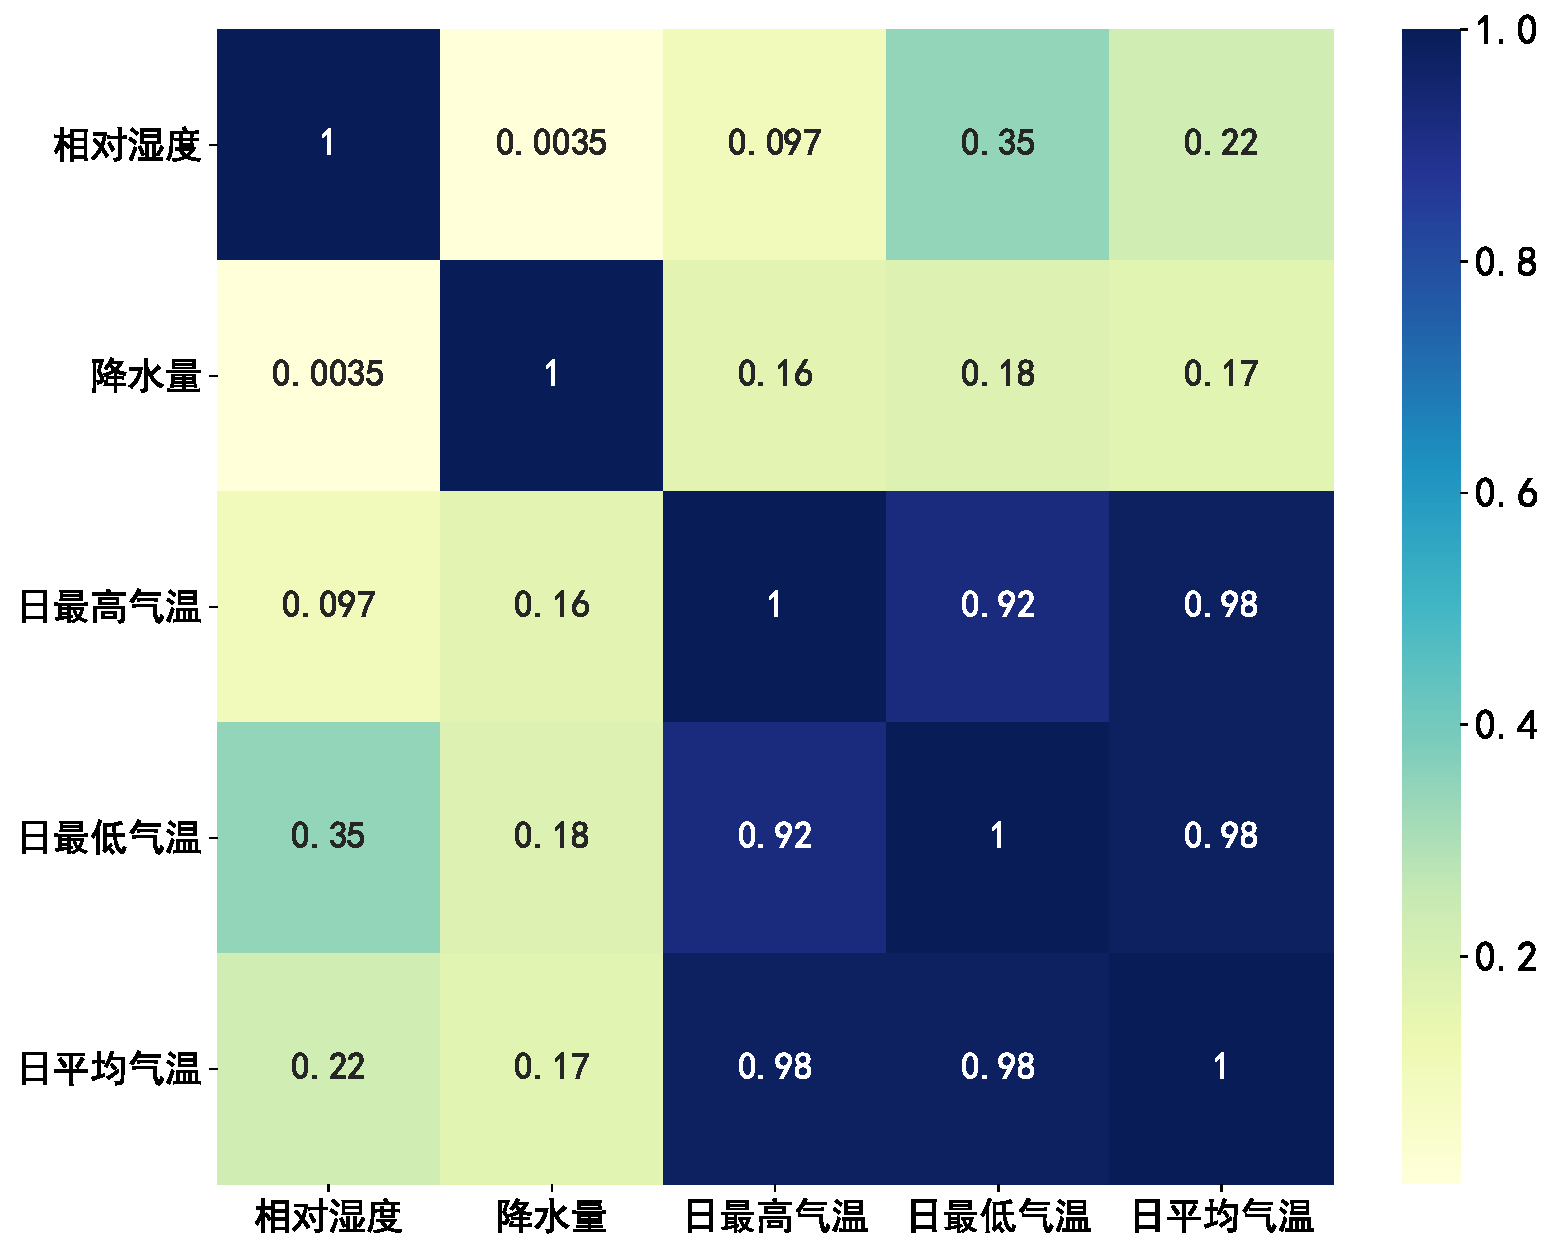
\includegraphics[width=0.7\textwidth]{./Img/相关性热力图.pdf}
  \caption{有效数据中不同指标间的相关性热力图}\label{fig:4-7-a}
\end{figure}

\begin{figure}[ht]
  \centering
  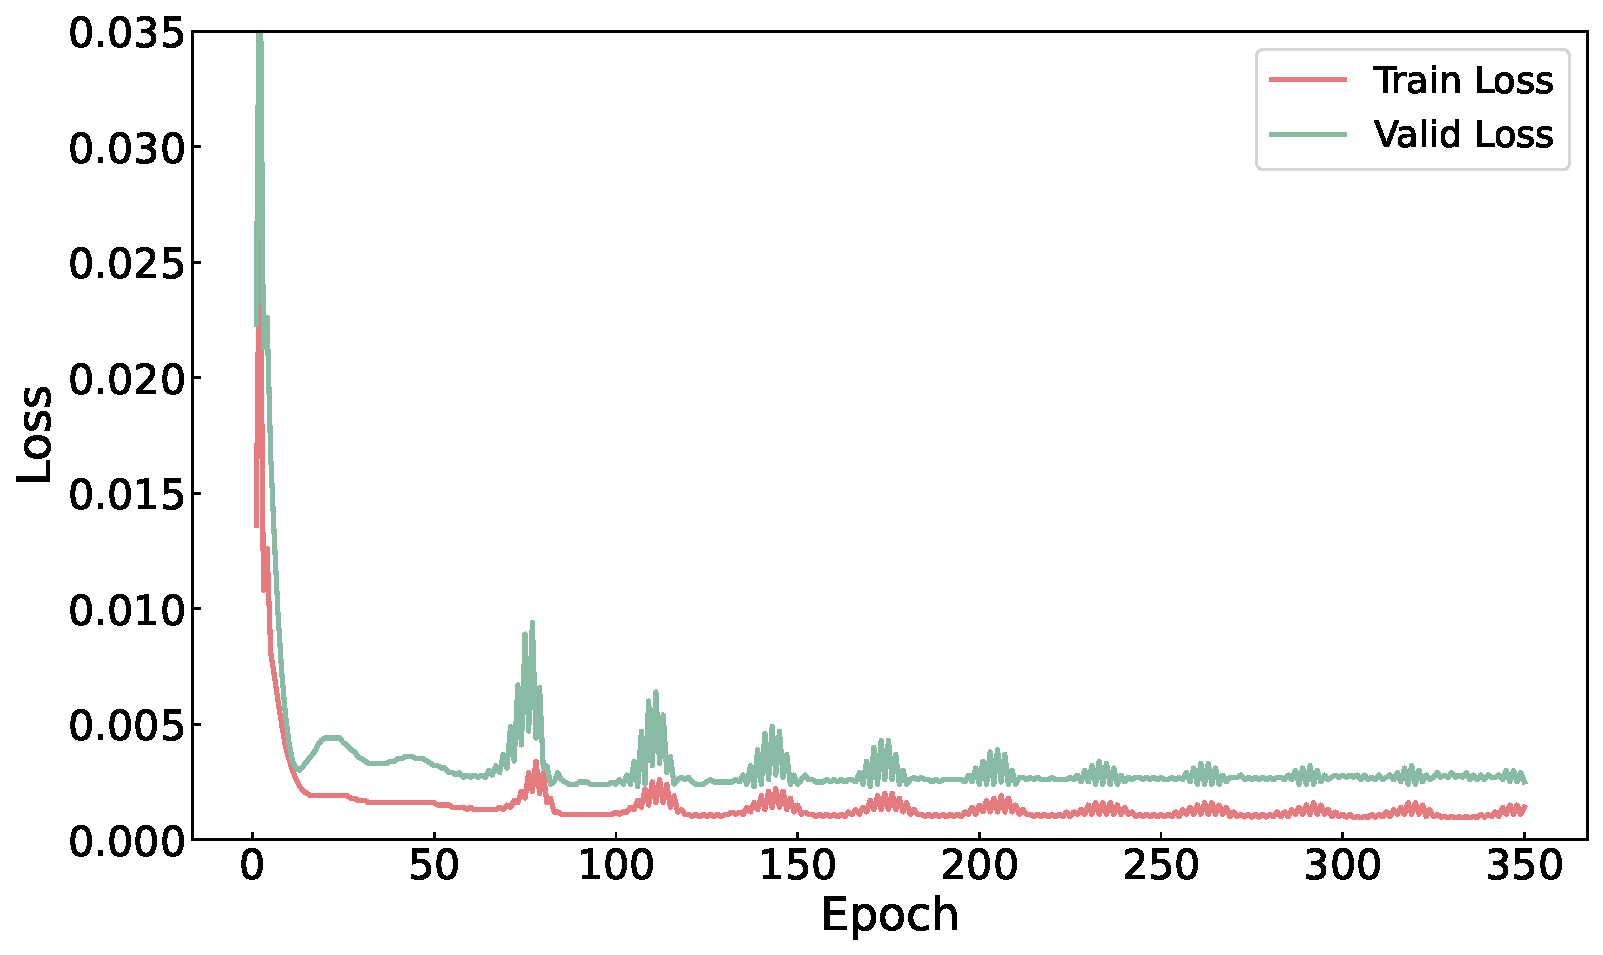
\includegraphics[width=0.7\textwidth]{./Img/LSTM_loss.pdf}
  \caption{LSTM模型的训练损失和验证损失}\label{fig:4-7}
\end{figure}

\begin{figure}[t]
  \centering
  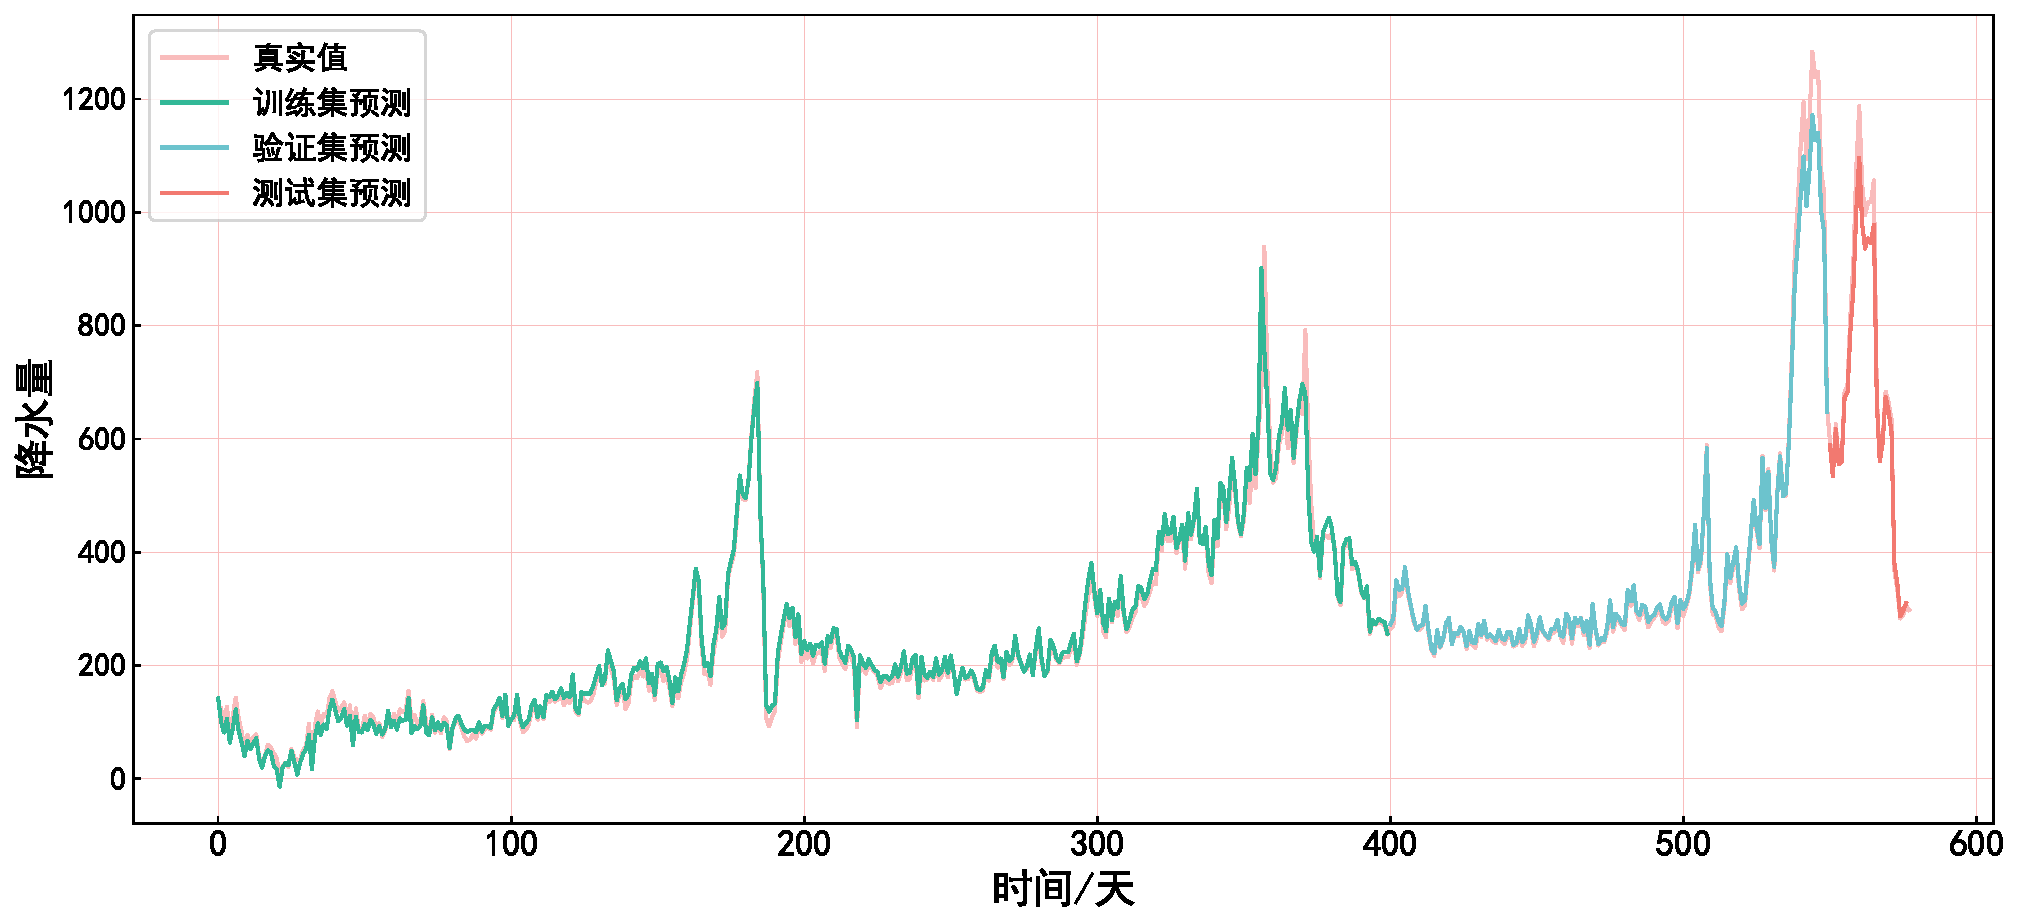
\includegraphics[width=1.0\textwidth]{./Img/LSTM_pre.pdf}
  \caption{LSTM模型针对三个数据集的预测结果}\label{fig:4-8}
\end{figure}

\begin{figure}[h]
  \centering
  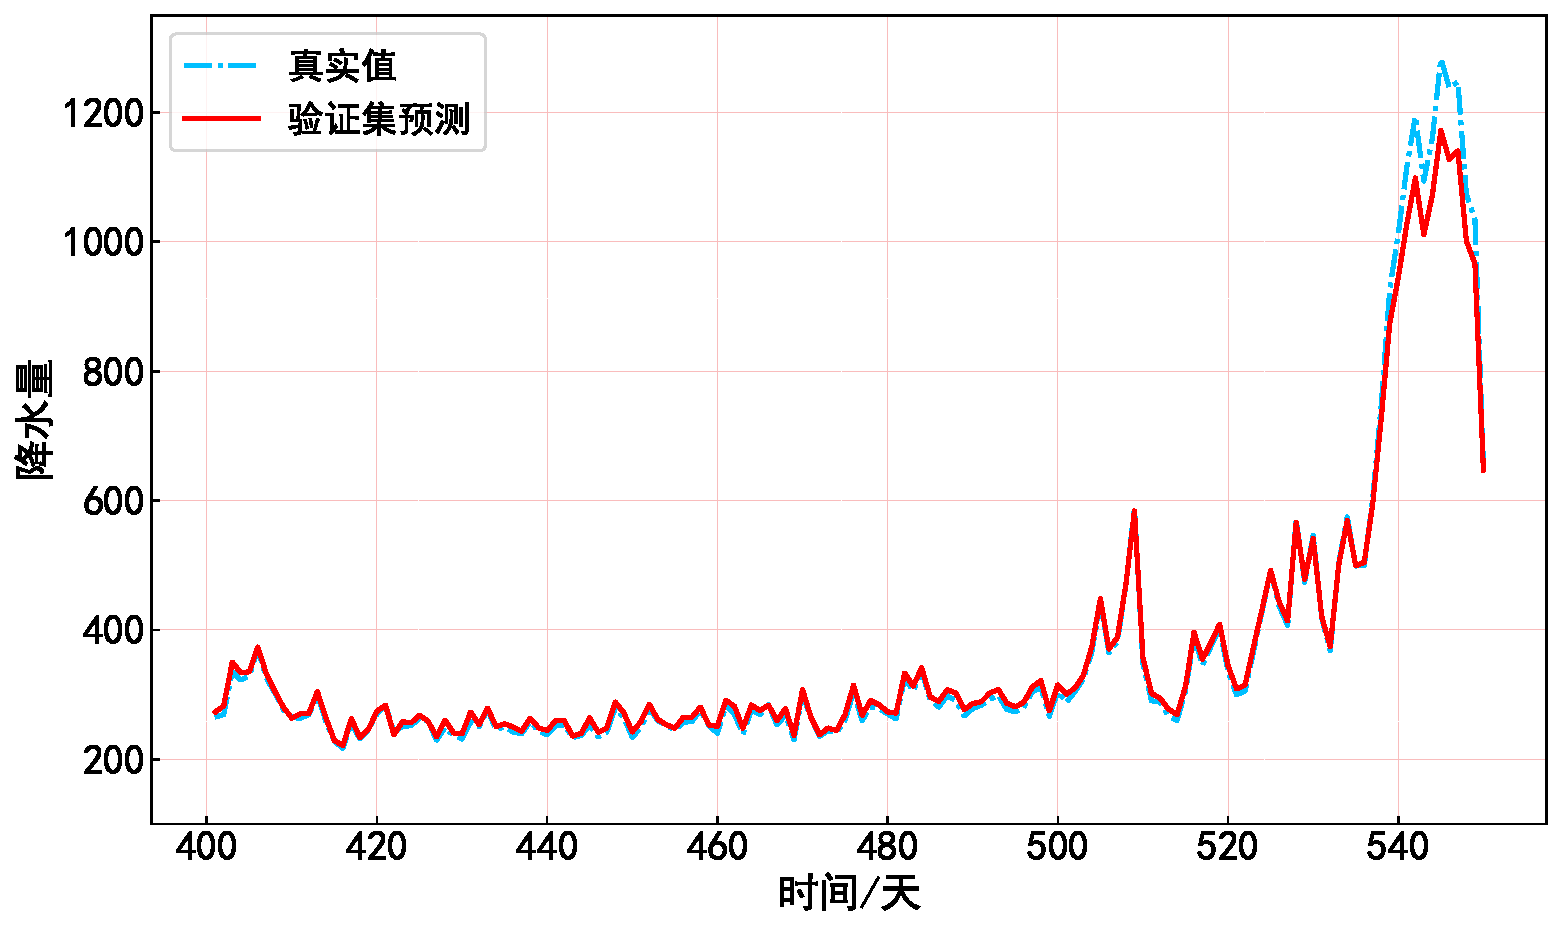
\includegraphics[width=0.7\textwidth]{./Img/LSTM_valid_pre.pdf}
  \caption{验证集预测结果与真实值对比}\label{fig:4-9}
\end{figure}

\begin{figure}[h]
  \centering
  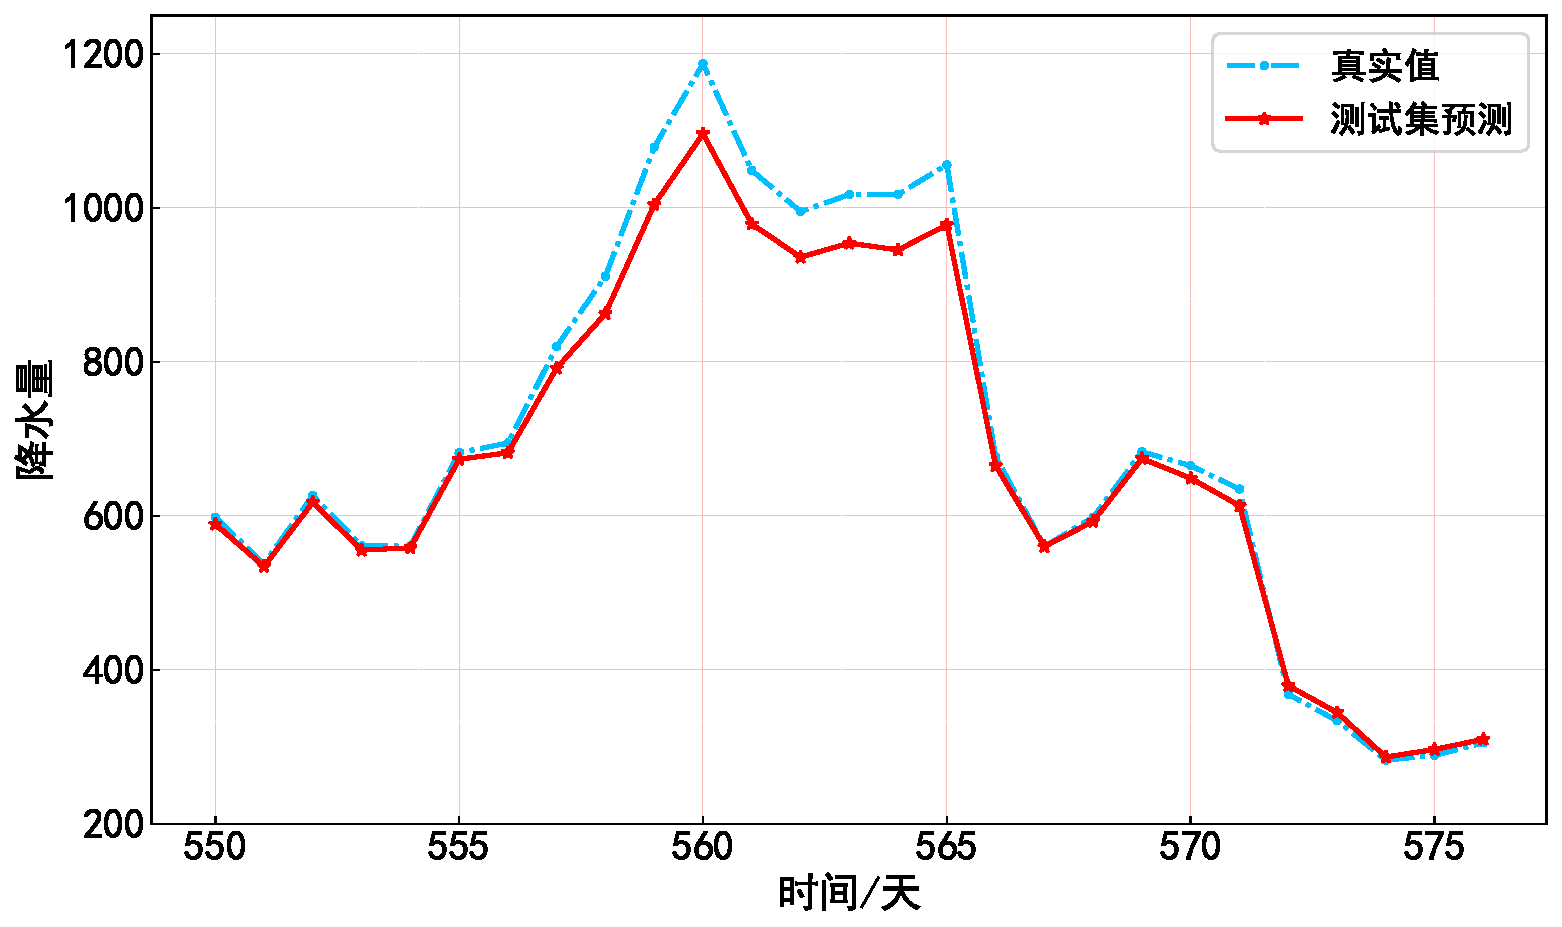
\includegraphics[width=0.7\textwidth]{./Img/LSTM_test_pre.pdf}
  \caption{测试集预测结果与真实值对比}\label{fig:4-10}
\end{figure}


如表 \ref{tab:LSTM_data——normalization} 得到归一化后的数据集之后,我们首先对日最高气温、日最低气温、日平均气温、相对湿度以及降水量组成的五个指标的特征集计算了相关性,得到的相关性的热力图如图 \ref{fig:4-7-a} 所示。观察图 \ref{fig:4-7-a} 可以看出,降水量与相对湿度的相关性微乎其微,仅0.0035,而与日最高气温、日最平均气温和日最低气温的相关性逐渐提升,但仍属中低水平,相关系数在0.16至0.18范围内。

值得注意的是,日最高气温、日最平均气温和日最低气温这三个指标由于属性相近和受到影响相同,因此彼此间存在极高相关性。整体上这些指标间展现了一种平衡状态,既体现了适度的相关性也保持了某种程度的互斥性,具备了一定的随机性,可以提高模型的泛化性能。

接下来,我们按照天数来划分训练集、测试集以及验证集,经过多次实验的测试,对不同的实验结果综合分析之后,选出了较优的划分区间,针对总共578天的数据,训练集我们选择 $[1,400]$ 这个天数区间作为训练,选择 $[401,549]$ 这个天数区间作为验证集,最后的 $[550,578]$ 这个区间作为测试集。在上一小节中,我们建立了LSTM模型,以降水量作为输出值,设定训练时epoch次数为350次,隐含层神经元的个数为1024个,训练时的每一批量大小为16,采用ReLU和Adam分别作为激活函数和优化器,经过上述的实验前提设定后,模型正式进入训练阶段,训练阶段的训练时损失和验证时损失如图 \ref{fig:4-7} 所示。训练完成后,使用训练好的模型分别针对训练集、验证集以及测试集进行模型推理,并将三个部分数据合并到一块,为了使各个部分有一定的区分,我们给训练集、验证集和测试集的预测结果以及真实值分别设置了不同的颜色,得到的结果如图 \ref{fig:4-8} 所示。

为清晰呈现验证集与测试集的预测效能,我们抽离了两者的数据,并分别在图 \ref{fig:4-9} 及图 \ref{fig:4-10} 中直观显现。从图中可以看出,在预测降水量方面,验证集的预测值与实测数据之间展现出高度吻合,有力证明了模型在此预测指标上的精确度。进一步深化对模型性能的分析,我们利用已训练完成的模型对[550, 575]天数范围内的数据进行了预测。预测结果的详细数据展示在表 \ref{tab:LSTM_data——pre} 中。


\begin{table}[h]
    \caption{模型针对[550,575]天降水量的预测结果}\label{tab:LSTM_data——pre}
    \centering
    \resizebox{1.0\linewidth}{!}
    {\begin{tabular}{*8{c}}\toprule
        时间 & 第550天 & 第555天 & 第560天 & 第565天 & 第570天 & 第575天 & ~ \\ 
        \midrule
        真实值 & 576.003 & 667.23314 & 1116.4658 & 1008.4208 & 660.2755 & 288.12021 \\ 
        预测值 & 556.38477 & 633.85547 & 1068.7562 & 953.265 & 622.2626 & 287.87445 \\ 
        误差 & 19.618 & 33.37767 & 47.7096 & 55.1558 & 38.0129 & 0.2458 \\ 
        误差占比 & 0.03406 & 0.05002 & 0.04273 & 0.05470 & 0.05757 & 0.000853 \\ 
        \bottomrule
    \end{tabular}}
\end{table}

最后,我们对测试集的预测值与实际观测值进行了误差分析,通过计算平均绝对百分比误差(MAPE),我们得出了总误差为23.994\%,而平均误差则为4\%。这一结果为我们评估模型在未知数据集上的泛化能力提供了重要依据。


% 综上所述,并结合图 \ref{fig:4-9}、图 \ref{fig:4-10} 以及表 \ref{tab:LSTM_data——pre} 的详细对比分析,结果清晰显示了预测趋势线与实际观测数据的近乎重合。不仅在趋势方向和波动幅度上高度一致,而且在关键的转折点及平均误差的表现上也呈现出高度一致性和较低误差,这充分证明了模型具有出色的预测性能。

综上所述,并结合图 \ref{fig:4-9}、图 \ref{fig:4-10} 以及表 \ref{tab:LSTM_data——pre} 中所展示的数据,我们可以进行一项详尽的对比分析。该分析的结果明确地揭示了本研究所提出的模型在预测气象数据方面的卓越性能。具体来说,预测趋势线与实际观测数据之间展现出了显著的一致性,这一点在趋势方向、波动幅度以及关键转折点的准确捕捉上均得到了体现。此外,模型在平均误差的表现上也极为出色,误差值保持在较低水平,进一步印证了模型的高预测精度。这一结果不仅证实了模型在处理复杂气象数据时的有效性,而且也表明了其在实际应用中的潜力。通过对模型预测结果与实际观测值之间的细致比较,我们能够得出结论:所提出的模型不仅能够准确地捕捉到气象数据的变化趋势,而且在细节层面上也能与实际观测保持高度一致,这对于提高气象预测的准确性和可靠性具有重要意义。

\subsubsection{创新研究}

\begin{figure}[h]
  \centering
  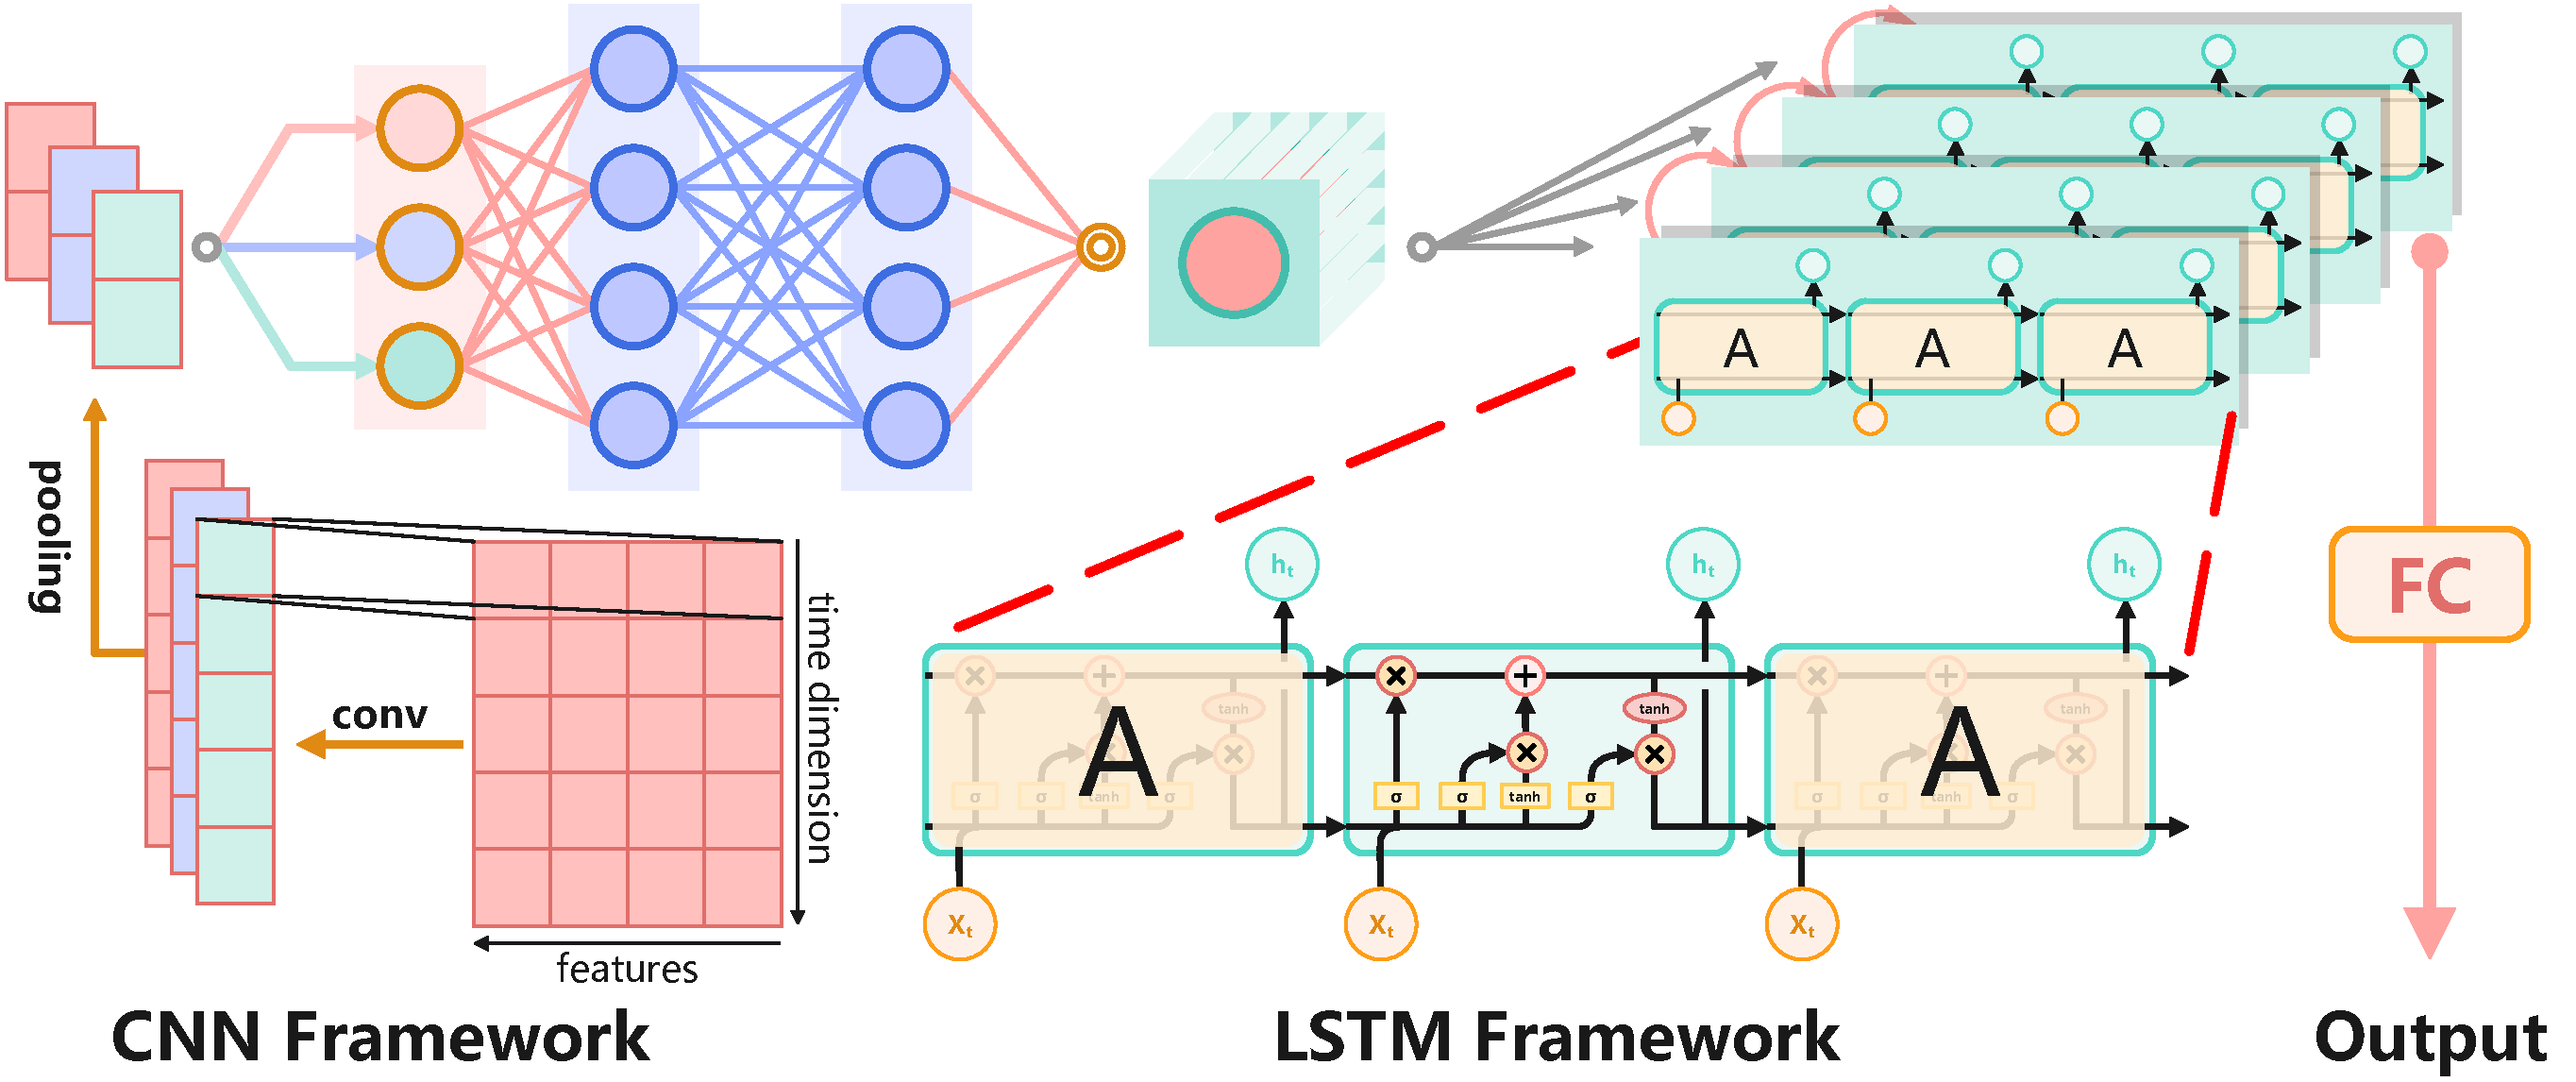
\includegraphics[width=1.0\textwidth]{./Img/CNN_LSTM结构图.pdf}
  \caption{CNN-LSTM整体结构图}\label{fig:4-11}
\end{figure}

当前气象研究领域的先进方法当中,目前较为流行的方法是融合了卷积神经网络(CNN)与长短时记忆网络(LSTM)的混合模型 \cite{HJKZ2024011600J}\cite{JYGC20240415002},大量的实验结果表明这种混合模型可以显著提高预测的准确性。受CNN-LSTM混合模型思想的启发,我们在LSTM模型的基础之上,引入了CNN网络,旨在于把时间序列数据转换成图像并使用深度学习技术来提取特征能够有效捕捉气象数据中的时间序列非线性变化,CNN与LSTM结合之后实际的架构设计如图 \ref{fig:4-11} 所示。





\begin{figure}[h]
  \centering
  \begin{subfigure}{0.48\textwidth}
      \centering
      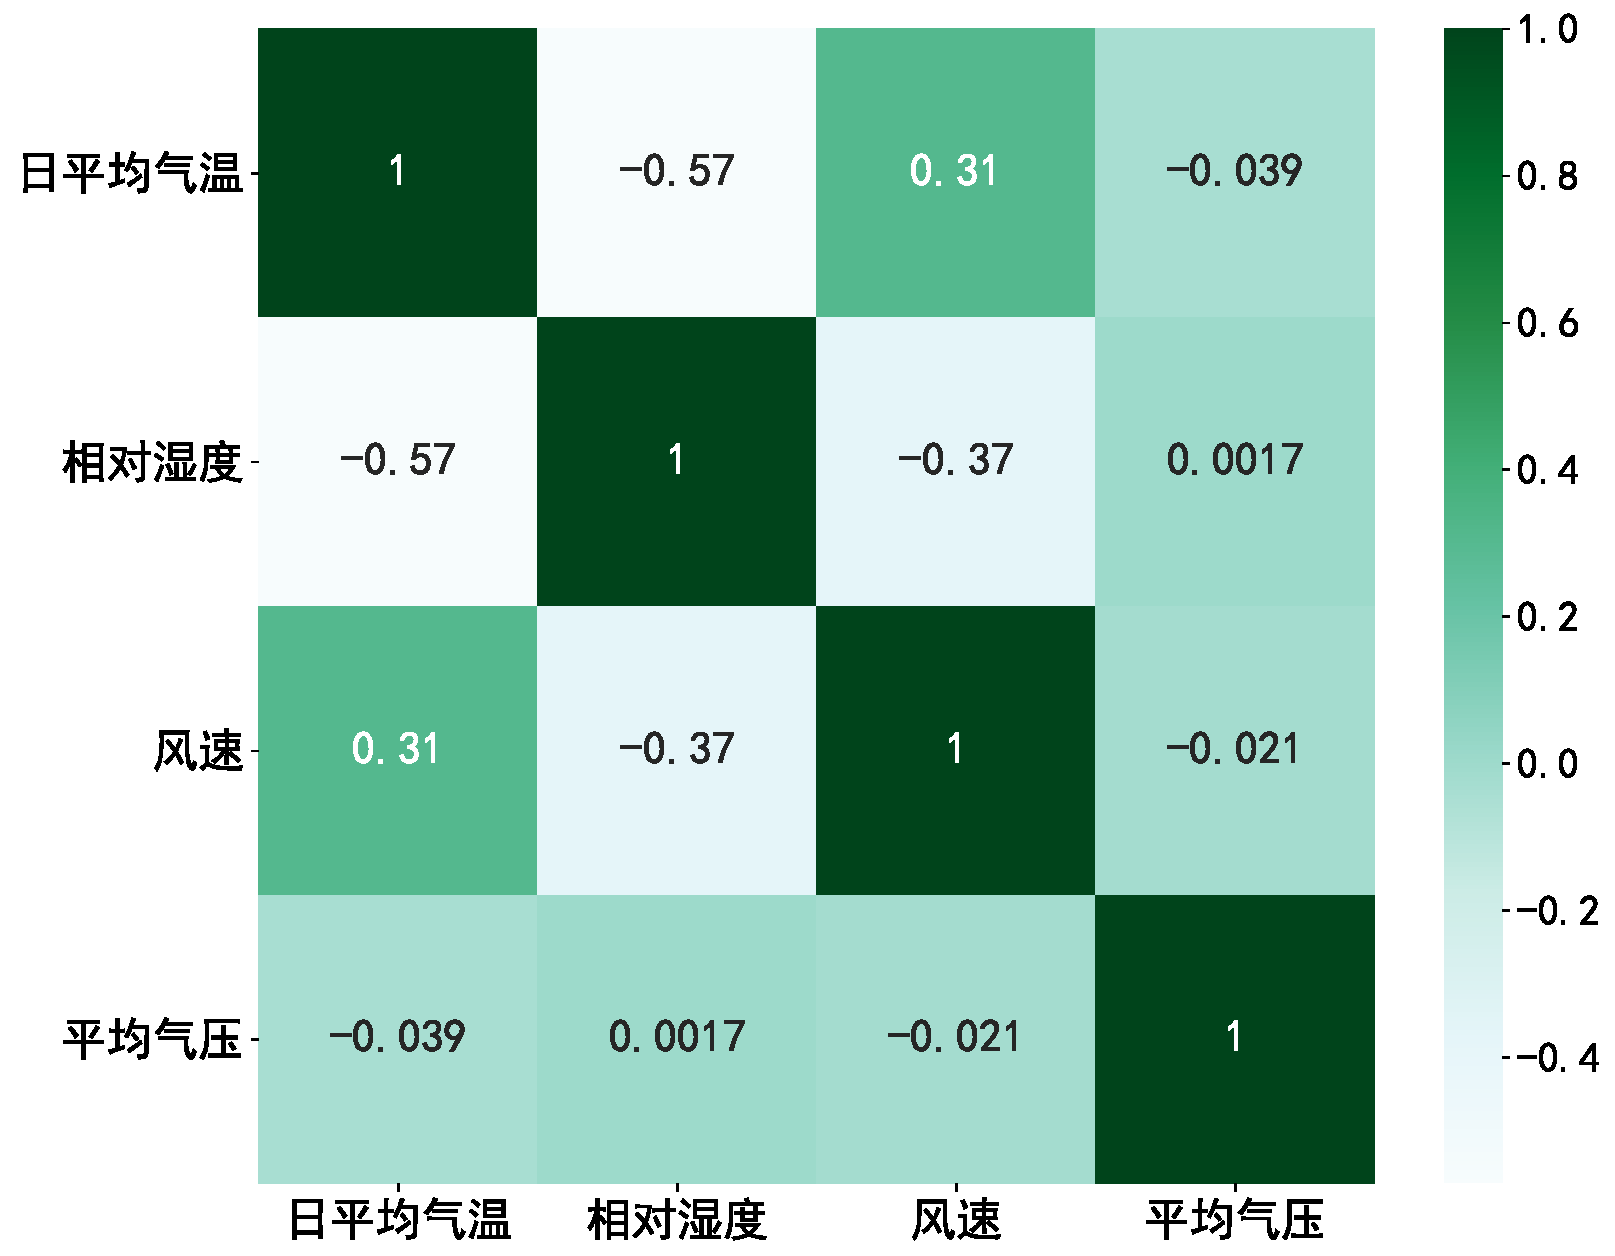
\includegraphics[width=\linewidth]{./Img/CNN-LSTM相关性热力图.pdf}
      \caption{有效数据中四项指标的相关性热力图}\label{fig:4-13-b}
  \end{subfigure}
  \hfil
  \begin{subfigure}{0.48\textwidth}
      \centering
      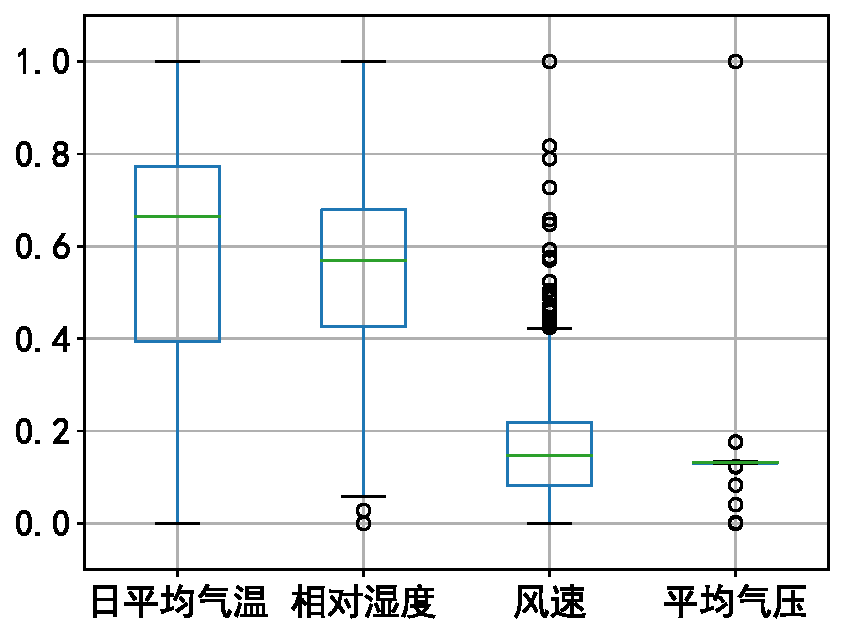
\includegraphics[width=\linewidth]{./Img/CNN-LSTM相关性箱线图.pdf}
      \caption{有效数据中四项指标的箱型图}\label{fig:4-13-c}
  \end{subfigure}
  \caption{四项指标的相关性热力图与箱型图}
  \label{fig:4-17-b}
\end{figure}




对于新的CNN-LSTM框架,为了更好的评估新框架的预测性能,我们严谨选择了新的一组气象数据作为数据集,新的数据集涵盖了2013年1月至2017年4月这段时间日平均气温、相对湿度、风速以及平均气压等指标的气象数据,为了深入探讨特征随机性对模型泛化能力的影响,我们采用了相关性热力图和箱型图这两种可视化工具,如图 \ref{fig:4-13-b} 和 \ref{fig:4-13-c} 所示,以便直观地揭示了不同指标之间的相关性和随机波动关系。

\begin{table}[h]
    \caption{2013年1月-2017年4月期间的有效气象数据}\label{tab:CNN_LSTM_data}
    \centering
    \resizebox{0.8\linewidth}{!}
    {\begin{tabular}{*5{c}}\toprule
        时间 & 日平均气温(${}^{\circ}\text{C}$) & 相对湿度($\%RH$) & 风速($m/s$)  & 平均气压($P_a$) \\ 
        \midrule
        2013-01-01 & 10.0 & 84.5 & 0.0 & 1015.67 \\
        2013-01-02 & 7.4 & 92.0 & 2.98 & 1017.8 \\
        2013-01-03 & 7.17 & 87.0 & 4.63 & 1018.67 \\
        2013-01-04 & 8.67 & 71.33 & 1.23 & 1017.17 \\
        2013-01-05 & 6.0 & 86.83 & 3.70 & 1016.5 \\
        2013-01-06 & 7.0 & 82.8 & 1.48 & 1018.0 \\
        2013-01-07 & 7.0 & 78.6 & 6.30 & 1020.0 \\
        2013-01-08 & 8.86 & 63.71 & 7.14 & 1018.71 \\
        $\cdots$ & $\cdots$ & $\cdots$ & $\cdots$ & $\cdots$ \\
        2017-04-18 & 34.0 & 27.33 & 7.81 & 1003.11 \\
        2017-04-19 & 33.5 & 24.13 & 9.03 & 1000.88 \\
        2017-04-20 & 34.5 & 27.50 & 5.56 & 998.63 \\
        2017-04-21 & 34.25 & 39.38 & 6.96 & 999.88 \\
        2017-04-22 & 32.90 & 40.90 & 8.90 & 1001.60 \\
        2017-04-23 & 32.88 & 27.50 & 9.96 & 1002.13 \\
        2017-04-24 & 32.00 & 27.14 & 12.16 & 1004.14 \\
        \bottomrule
    \end{tabular}}
\end{table}

在相关性热力图 \ref{fig:4-13-b} 中,我们可以观察到日平均气温与相对湿度之间存在中等到较强的负相关性(-0.57),而与风速之间则有轻微的正相关性(0.31),与气压的相关性则几乎可以忽略不计。此外,风速和相对湿度之间的相关性为中等程度的负相关(-0.37)。在箱型图 \ref{fig:4-13-c} 中,日平均气温和相对湿度的分布较为集中,且大部分数据位于中间位置,说明这两个变量的取值相对稳定。风速的分布则呈现出较大的差异,数据分散在较宽的范围内,说明风速的变化较大。平均气压的分布也轻度分散,整体上取值较低,说明平均气压的值相对较小。总体来看,这四个指标之间展现出了复杂而多样的相关性模式,既有正相关也存在负相关,这不仅丰富了模型对这些指标相互依赖关系和潜在影响的理解,而且有助于提升模型的泛化性能。通过这种方式,我们确保了模型在面对未知数据集时,能够保持广泛的适用性和高度的可靠性。


在模型训练之前,我们首先对数据进行了预处理。同样遵循LSTM模型的数据预处理规范,我们对数据集中出现的缺失值和异常值采取了均值填补策略,剔除了缺失超过三项气象指标的数据记录。经过数据处理步骤后,我们得到了1462条气象观测数据。这些数据包括了2013年至2017年的日平均气温。我们将整理后的数据部分以表格形式展示,如表 \ref{tab:CNN_LSTM_data} 所示。此外,我们还进行了数据可视化处理,可视化后日平均气温数据如图 \ref{fig:4-13-a} 所示。



\begin{figure}[h]
  \centering
  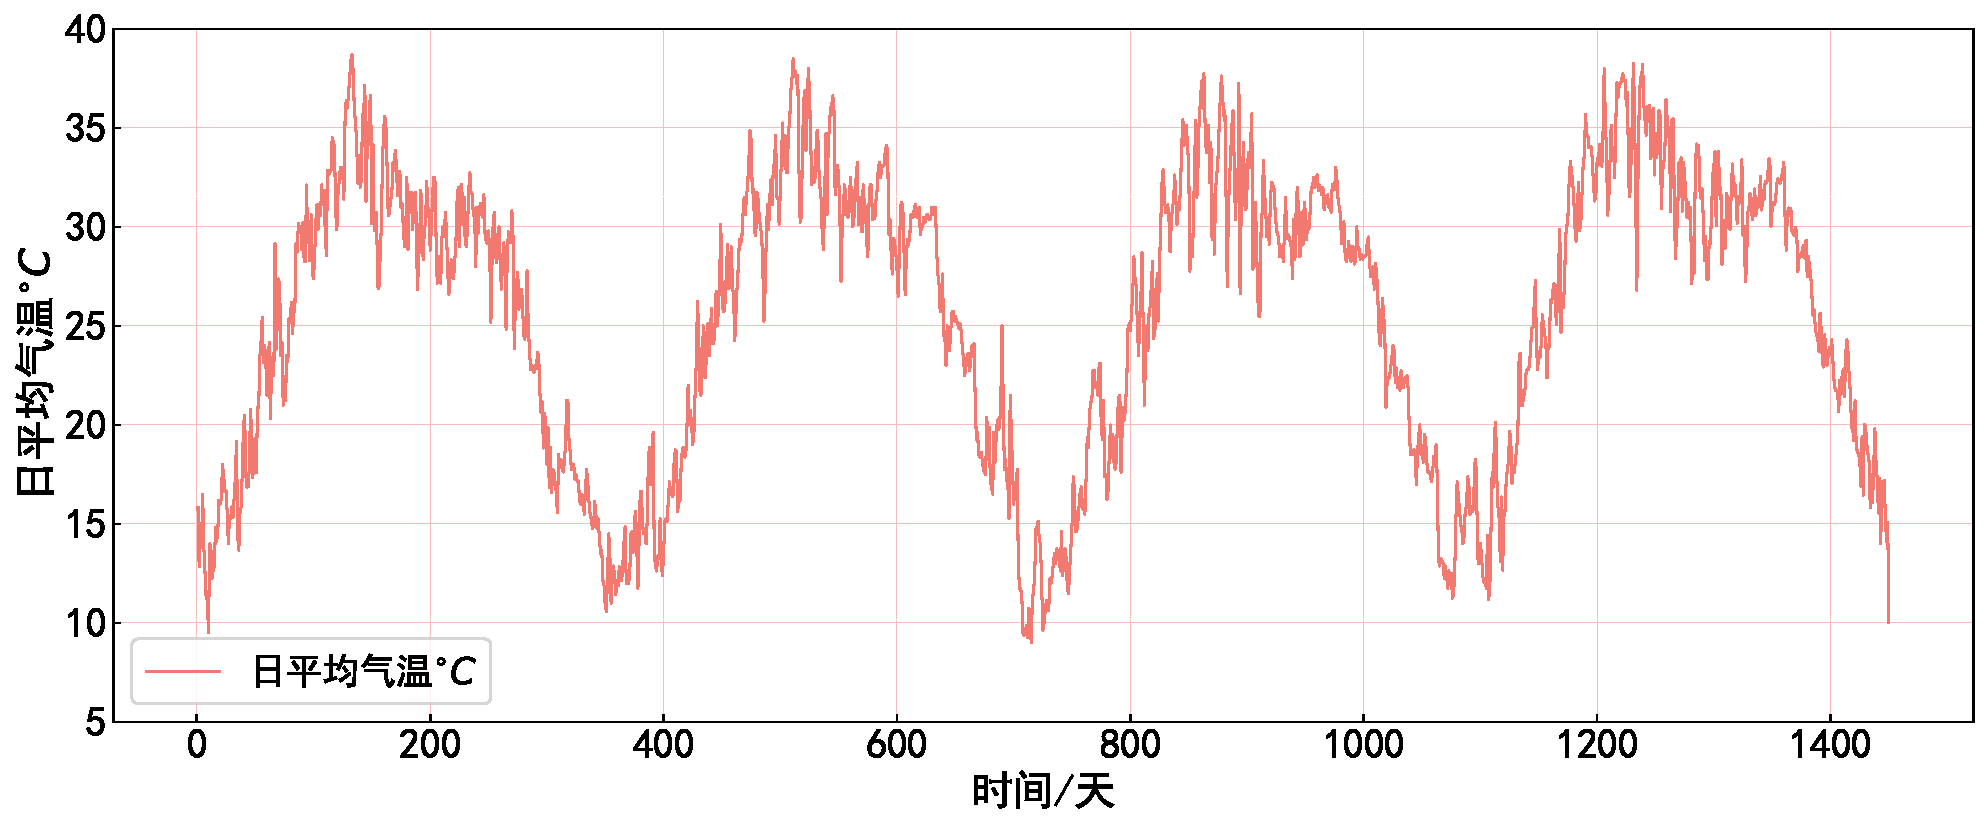
\includegraphics[width=1.0\textwidth]{./Img/CNN_LSTM_origin_data.pdf}
  \caption{2013年-2017年日平均气温}\label{fig:4-13-a}
\end{figure}


\begin{figure}[h]
  \centering
  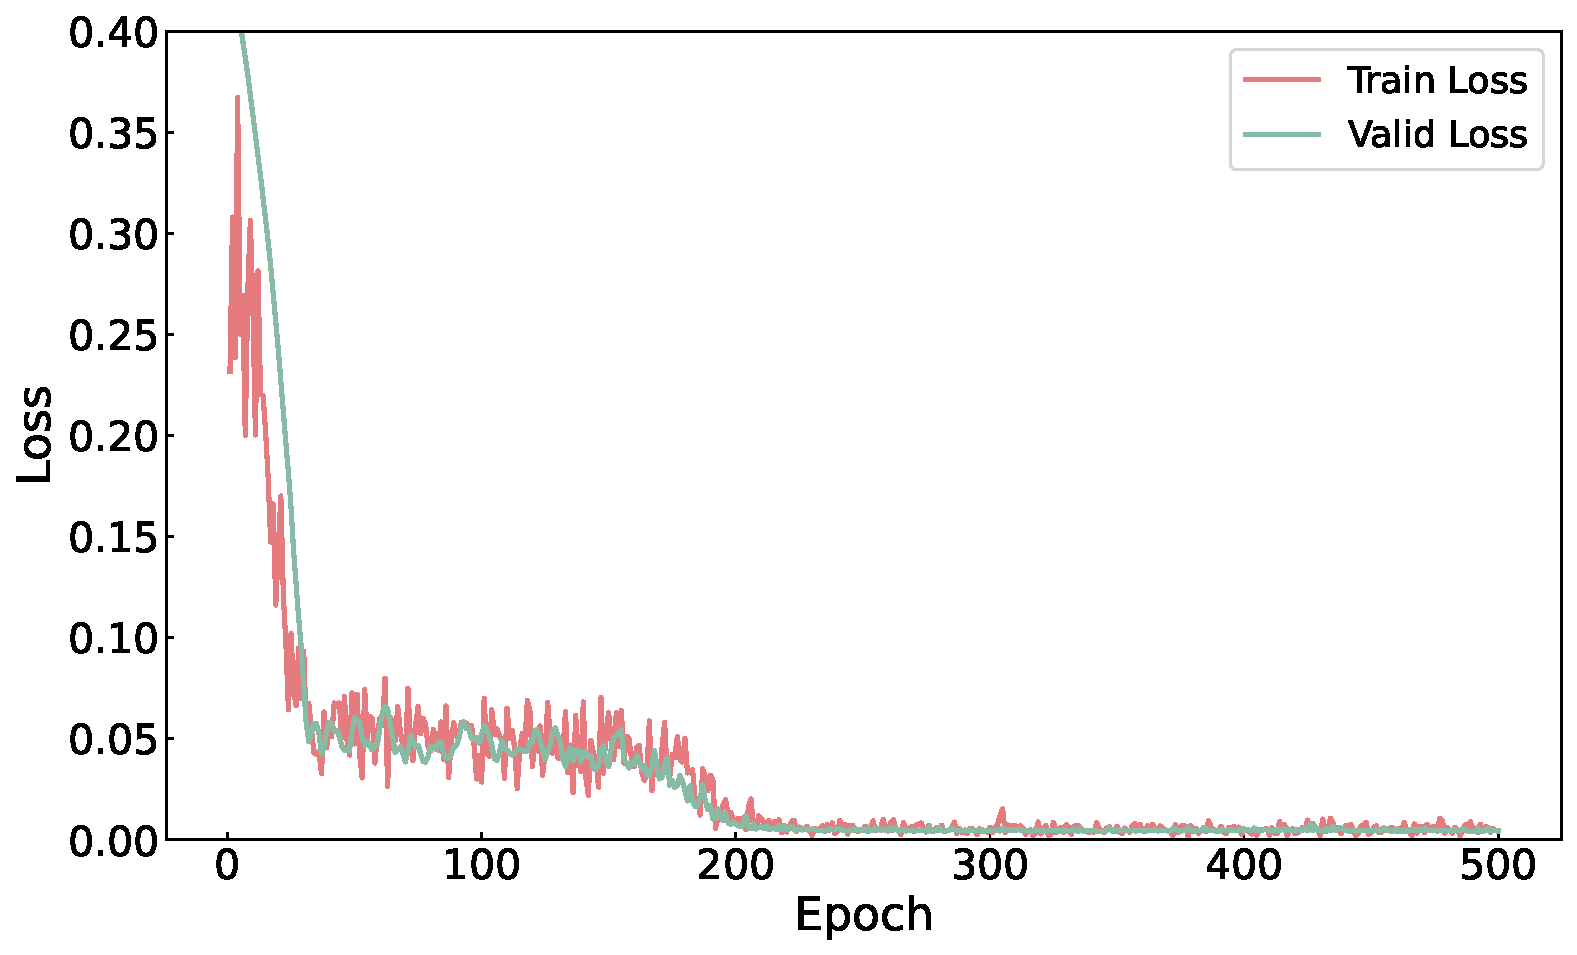
\includegraphics[width=0.7\textwidth]{./Img/CNN_LSTM_loss.pdf}
  \caption{CNN-LSTM模型的训练损失与验证损失}\label{fig:4-12}
\end{figure}



\begin{figure}[t]
  \centering
  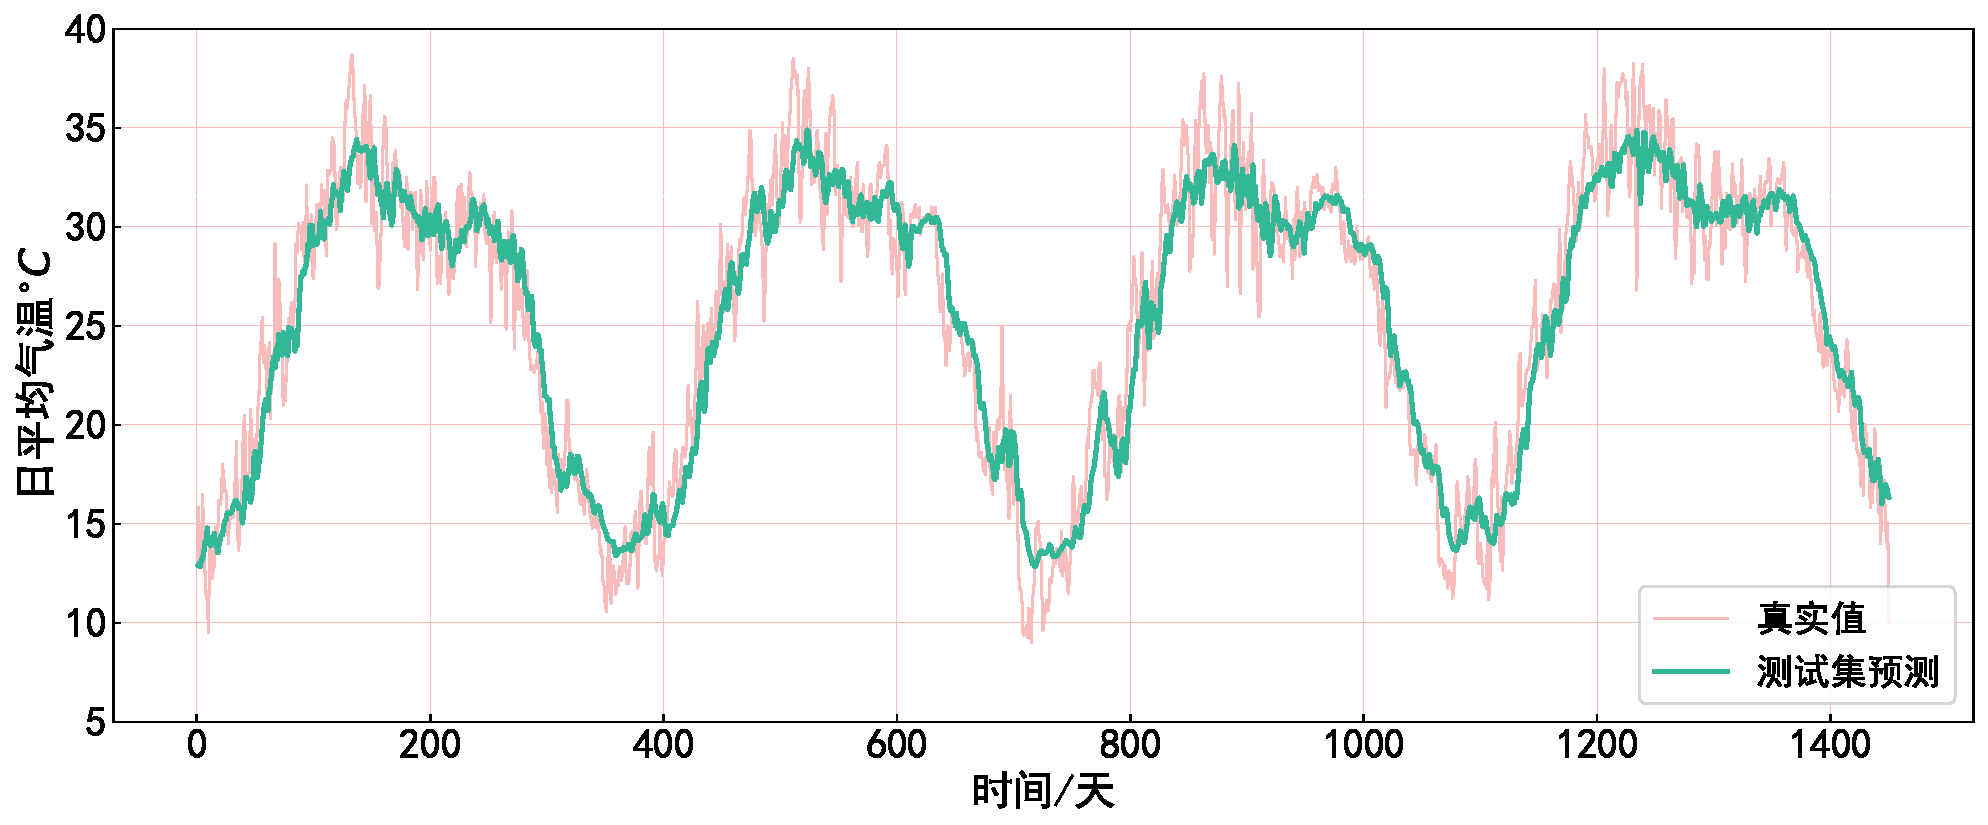
\includegraphics[width=1.0\textwidth]{./Img/CNN_LSTM_test_pre.pdf}
  \caption{CNN-LSTM模型针对2013-2017年日平均气温的预测结果}\label{fig:4-13}
\end{figure}


接下来,我们进入模型训练阶段,首先对所有数据执行了归一化处理,并选择了日平均气温作为关键的评价指标,设定的训练次数Epoch为500次,训练时的每一批量大小为16,采用ReLU和Adam分别作为激活函数和优化器。随后,将这些配置应用于CNN-LSTM模型中展开训练,模型训练过程的训练损失和验证损失如图 \ref{fig:4-12} 所示。在训练完成之后,进入模型推理阶段,使用训练好的模型针对指定时间段 [1,1462] 这个时间区间进行预测,得到的预测结果如图 \ref{fig:4-13} 所示,经过计算,得到预测值和真实值的均方误差为:$5.0165 {}^{\circ}\text{C}{}^2$。

\begin{figure}[h]
  \centering
  \begin{subfigure}{0.48\textwidth}
    \centering
    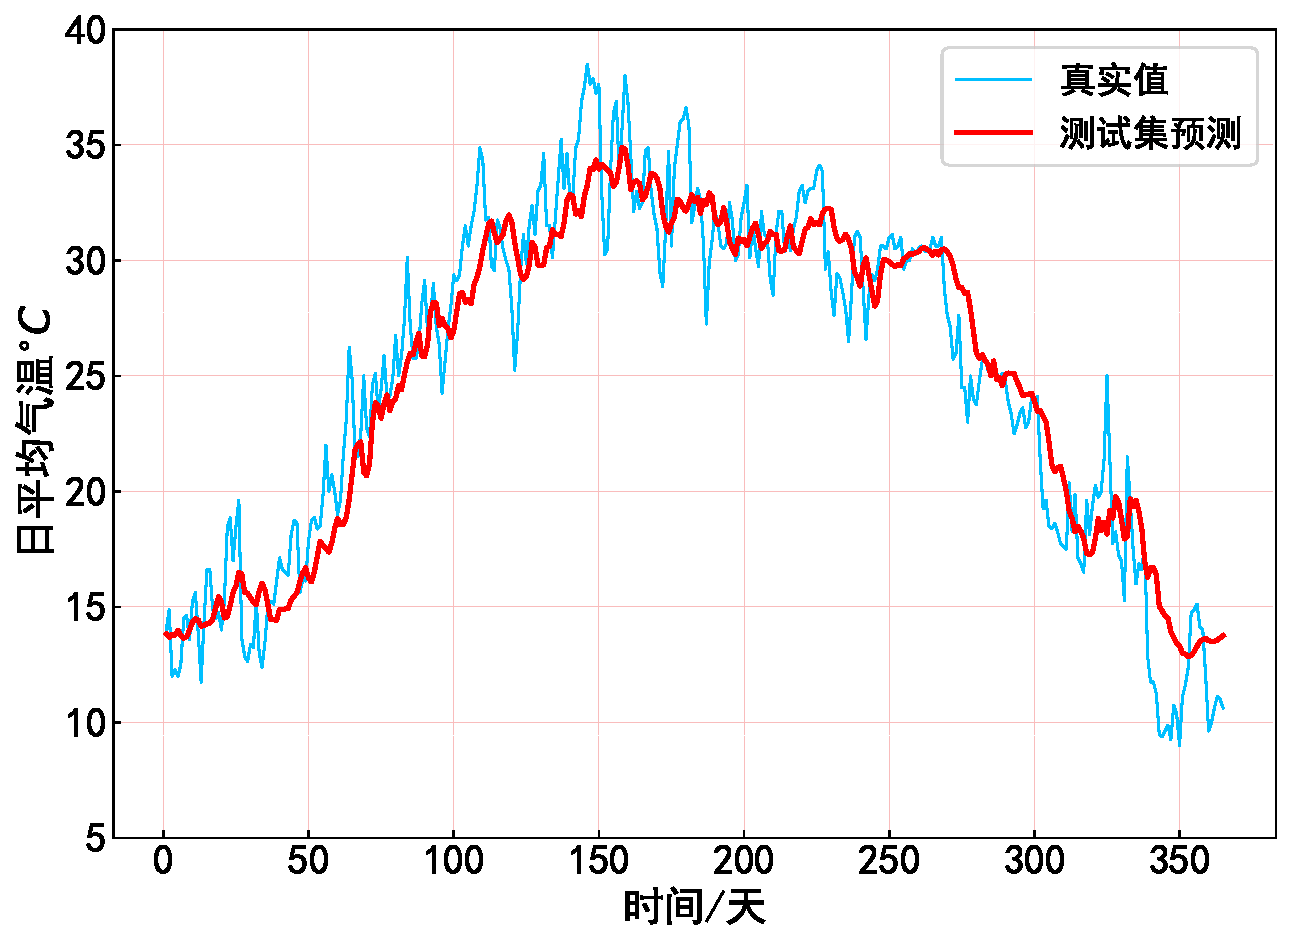
\includegraphics[width=\linewidth]{./Img/CNN_LSTM_test_first_pre.pdf}
    \caption{2014年全年日平均气温预测值与真实值对比}\label{fig:4-14}
  \end{subfigure}
  \hfil
  \begin{subfigure}{0.48\textwidth}
    \centering
    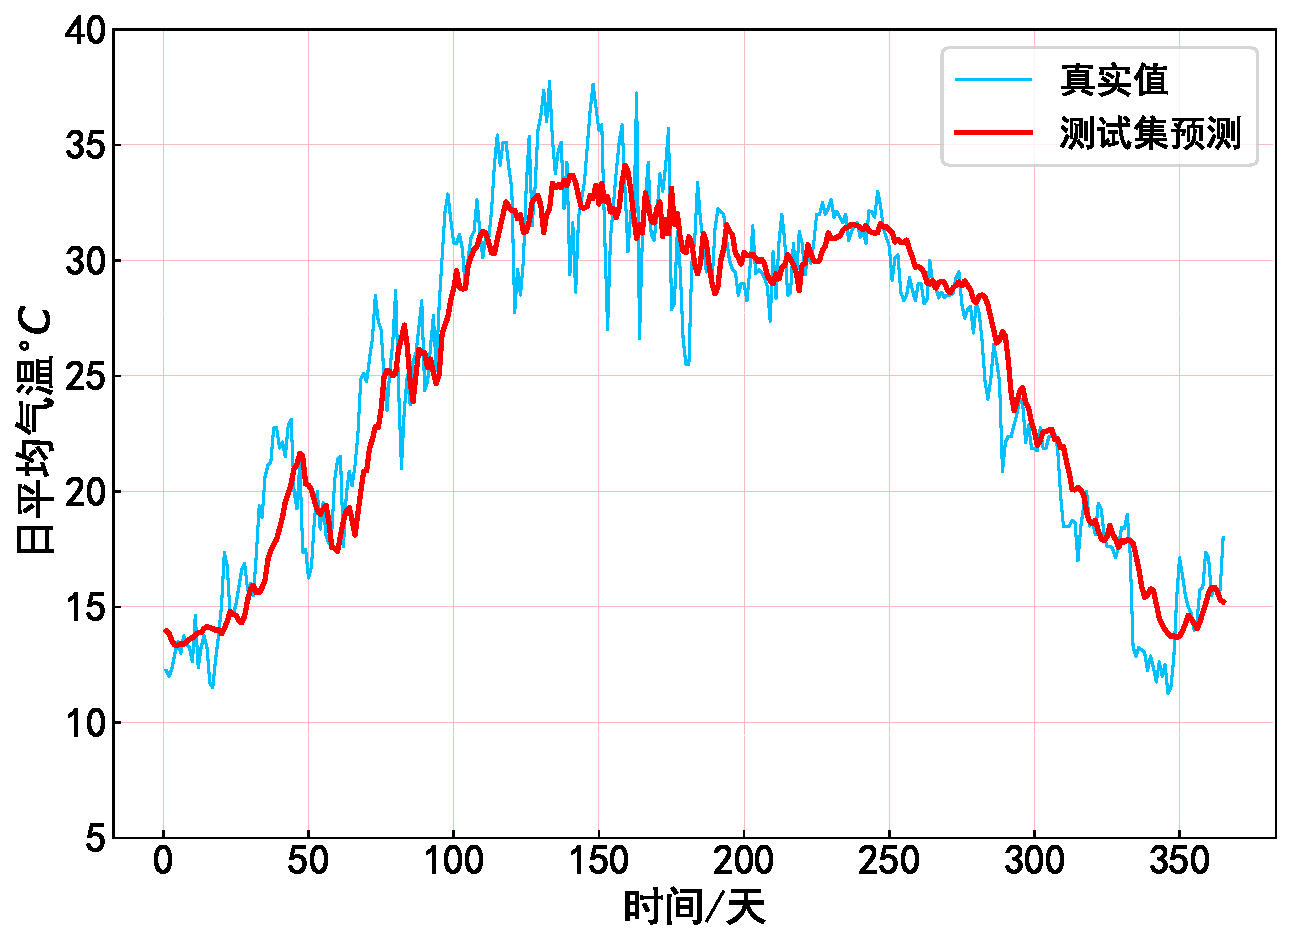
\includegraphics[width=\linewidth]{./Img/CNN_LSTM_test_section_pre.pdf}
    \caption{2015年全年日平均气温预测与真实值对比}\label{fig:4-15}
  \end{subfigure}
  \caption{2014年与2015全年日平均气温预测结果}
  \label{fig:4-17-all}
\end{figure}

在分析图 \ref{fig:4-13} 中的气象数据预测时,我们可以看到预测值与真实值整体上保持了较好的一致性,尤其是在日平均气温的预测中,模型能够较为准确地捕捉到温度的变化趋势。然而,在一些特定的时间段,如风速和平均气压的波动较大时,预测值与真实值之间存在一定的偏差。这可能意味着模型在这些情况下对风速和气压的处理不够精确,或者是模型过于专注于日平均气温的预测,而忽视了其他因素的综合影响。为了更清晰地显示真实值与预测值的差别,我们分别挑选出了2014年和2015年的全年日平均气温真实值和预测值进行可视化,如图 \ref{fig:4-17-all} 中的图 \ref{fig:4-14} 和图 \ref{fig:4-15} 所示。


此外,综合分析图 \ref{fig:4-8}、图 \ref{fig:4-9}、图 \ref{fig:4-10}、图 \ref{fig:4-13}、图 \ref{fig:4-14} 以及图 \ref{fig:4-15},单独的LSTM模型在小规模多个指标的数据集上表现出色,其预测结果与真实值的高度一致性和拟合程度不仅彰显了模型的强大泛化能力,也充分验证了我们在特征工程、模型架构设计以及超参数调优策略方面的有效性和准确性。然而,对于新型的CNN-LSTM架构,它在相对大型且少量指标的数据集上,尤其是在波动程度较大的数据,如极端天气事件前后,预测误差较大。这可能是因为模型未能充分学习到这些特殊情况下的特征,或者在处理异常数据时的鲁棒性不足。因此,为了提高预测精度,我们可以考虑对模型进行改进,例如引入更多的特征变量、优化模型结构或调整参数等。虽然当前的预测模型在一定程度上能够反映日平均气温的变化趋势,但在处理极端天气和其他影响因素时仍存在一些不足之处。未来的研究可以进一步探讨如何提高模型的预测能力,以更好地支持气象数据的分析和预报工作。



\subsection{LGESD细粒度哈希图像检索模型}

\subsubsection{模型介绍}

\begin{figure}[h]
  \centering
  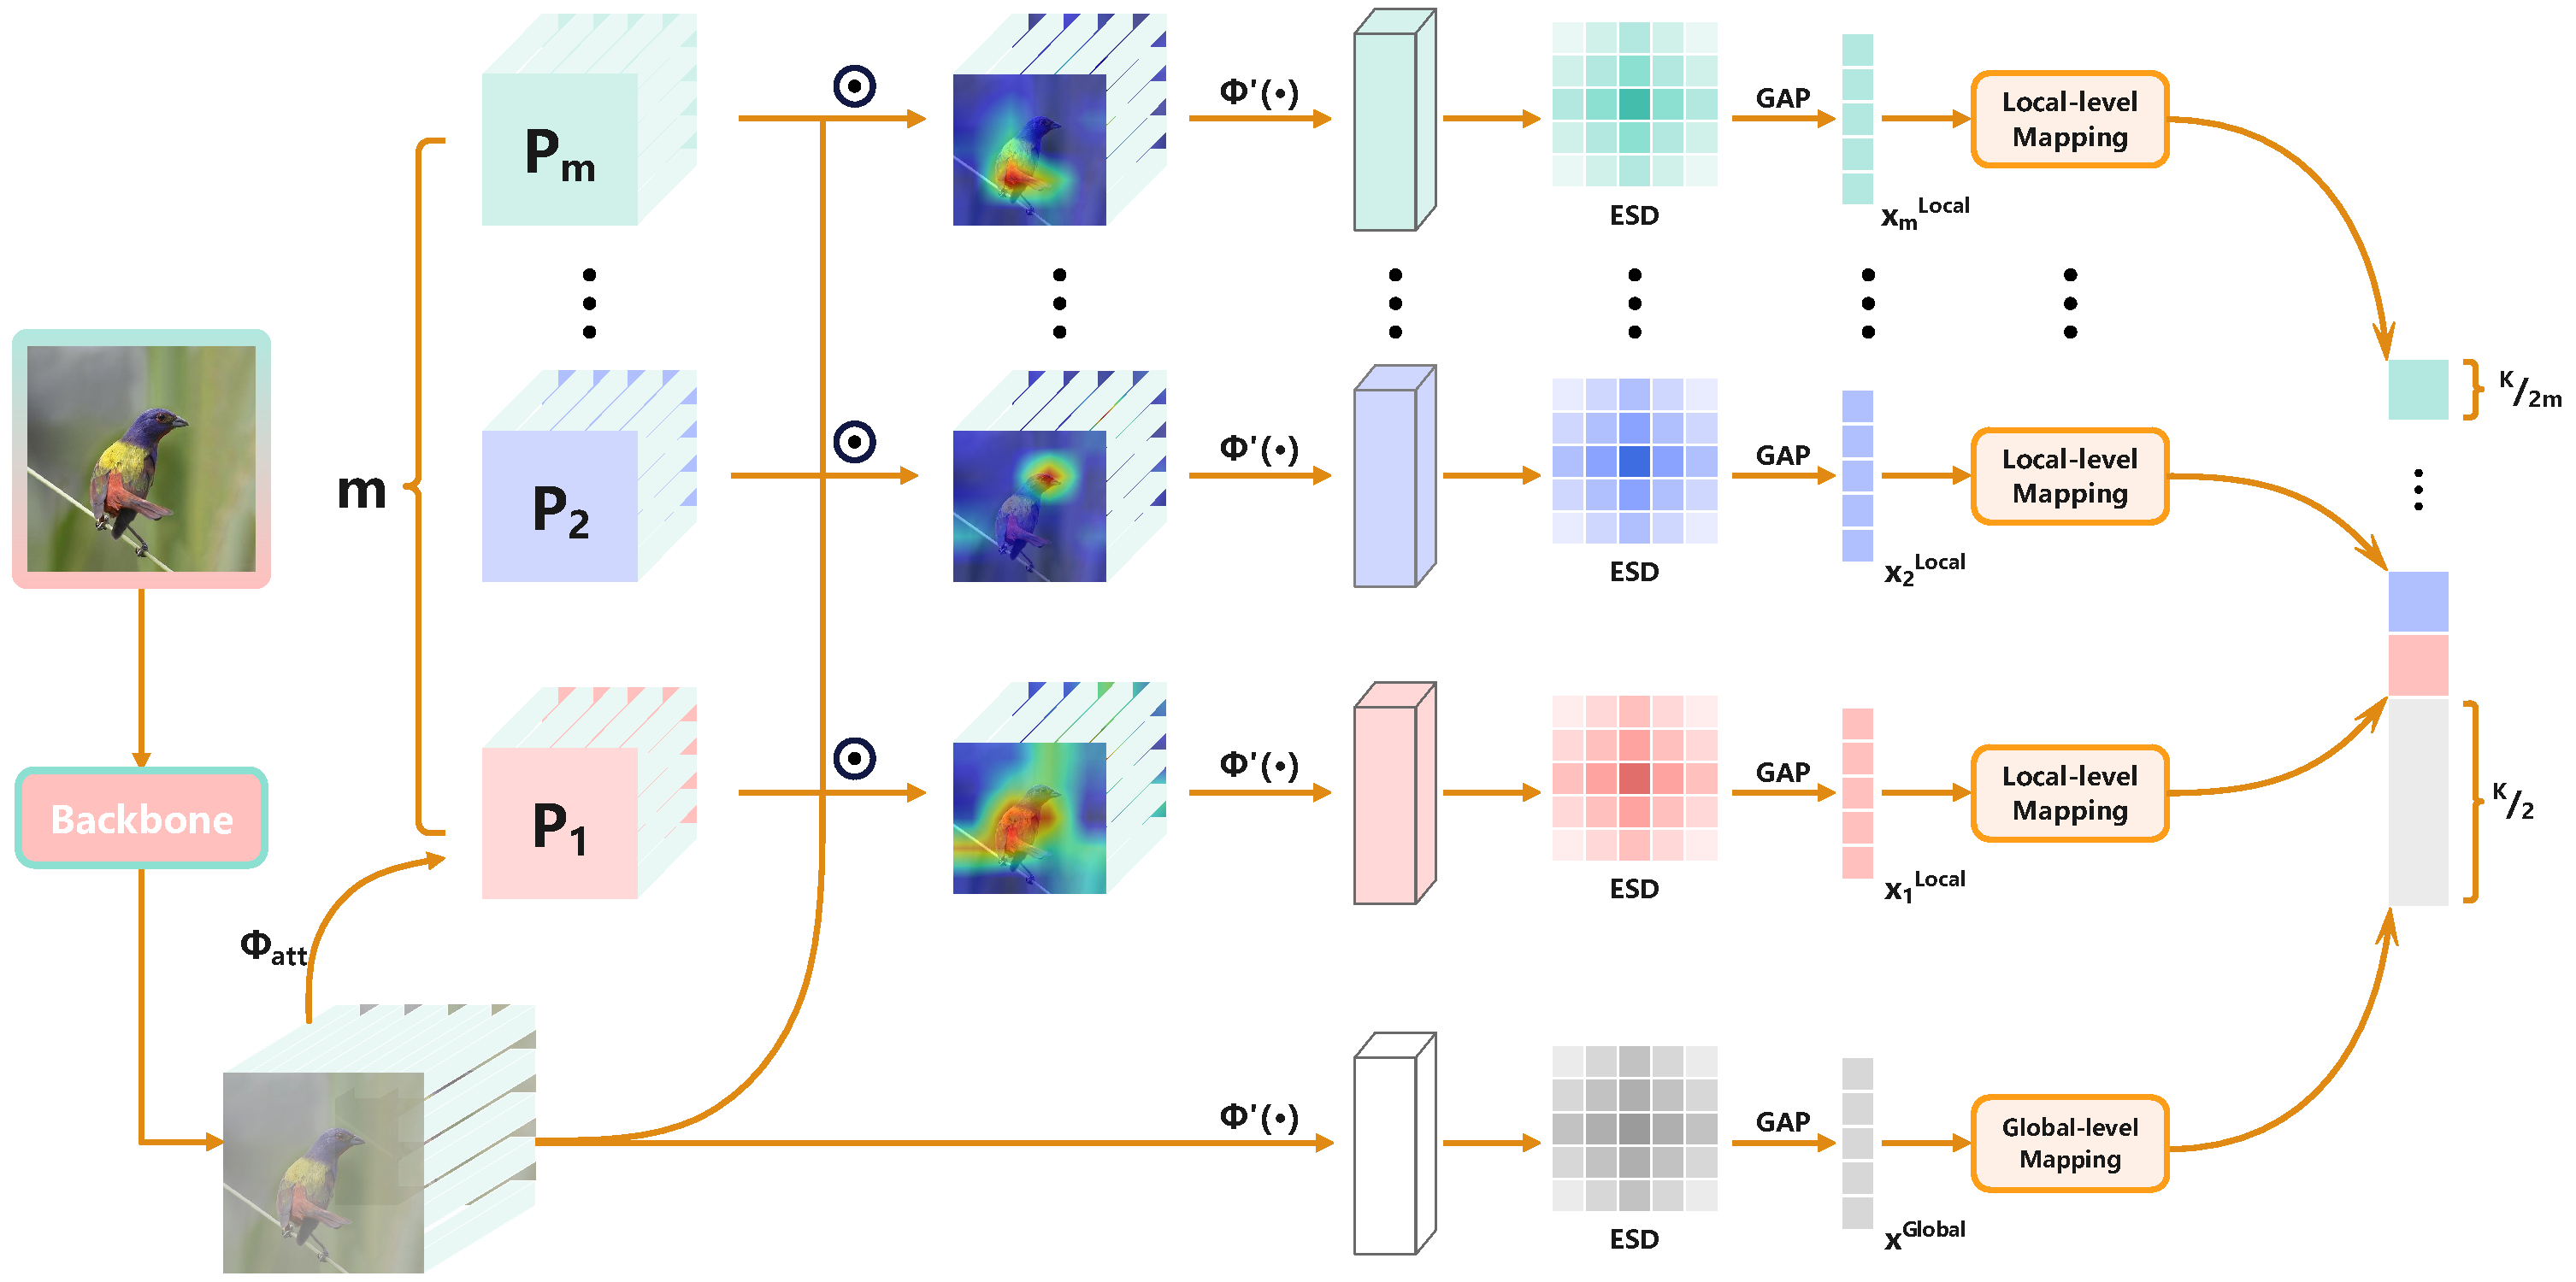
\includegraphics[width=1.0\textwidth]{./Img/完整架构图.pdf}
  \caption{LGESD整体架构图}\label{fig:4-21}
\end{figure}

通常情况下,在细粒度视觉识别任务中,兼顾对象的整体(全局)特征与局部细节(部分级)特征被认为是极为关键的 \cite{wei2021finegrained}。基于这一认识,我们提出了 \textbf{LGESD} 框架,一个基于显式空间衰减的局部与全局学习(\textbf{L}ocal and \textbf{G}lobal learning of \textbf{E}xplicit \textbf{S}patial \textbf{D}ecay)的细粒度哈希检索框架,我们在该框架中构建了一个双轨结构:一方面是一个专注于全局特征提取的学习分支,另一方面则是专攻局部模式学习的分支,架构详情如图 \ref{fig:4-21} 所示。在双轨结构设计的基础上,哈希码生成机制同样采用了双层设计,包含一个全局哈希映射单元和一个局部哈希映射单元。

其中,全局哈希映射单元旨在提炼反映对象整体信息的二进制码;而局部哈希映射单元则进一步细分,通过 $m$ 个子线性编码器模块来实现,专门用于明确提取每个组成部分的局部二进制哈希码,以此增强对细微特征的区分能力。因此,所得的哈希码内嵌了物体的全局身份信息与局部结构特征。此外,我们在该框架中创新性的引入了一种基于显式超先验的空间衰减注意机制(\textbf{E}xplicit \textbf{S}patial \textbf{D}ecay,\textbf{ESD}),该机制在下游处理阶段发挥着核心作用,确保生成的全局特征与对应局部特征既能互补又能凸显各自的独特性,从而提升特征表达的辨别力。

\subsubsection{整体框架设计}

对于输入的每一张图像 $\mathrm{I}$,经过一个卷积神经网络 $\Phi_{\mathrm{CNN}}(\cdot)$ 提取出它的深度激活张量 $\mathrm{T}$:
\begin{equation}
    \mathrm{T}=\Phi_{\mathrm{CNN}}(\mathrm{I})\in\mathbb{R}^{C\times H\times W}
\end{equation}

基于深度激活张量 $\mathrm{T}$,在全局特征学习分支中执行配备一叠卷积层的全局级转换网络 $\phi(\cdot)$,如下所示:
\begin{equation}
\hat{\mathrm{T}}=\phi(\mathrm{T};\theta_{\mathrm{global}})\in\mathbb{R}^{C^{\prime}\times H^{\prime}\times W^{\prime}}
\end{equation}

其中 $\theta_{\mathrm{global}}$ 表示 $\phi(\cdot)$的参数配置,而在局部特征学习当中,分别划分了 $m$ 个学习阶段,并为每一个学习阶段的添加了一个注意力引导机制 $\mathrm{P}_i = \phi_{\mathrm{att}}(T;\theta_{\mathrm{att}}), \mathrm{P}_i \in \mathrm{R}^{\frac{C}{m} \times H \times W}$,用于在每个阶段学习生成注意力图 $M_i$,在得到每个学习阶段注意力图之后,通过逐个元素点乘的方式评估 $H \times W$ 个元素当中被关注的深度描述符。
\begin{equation}
    \mathrm{T}_i^{\prime}=M_i\odot \mathrm{T}, \quad i \in \{1,2,\cdots,m \}
    \label{eq:eq_4_m}
\end{equation}

获得深度描述符之后,为了获得特定于语义的表示,我们选择使用与 $\phi(\cdot)$ 具有相同结构的局部级变换网络 $\phi^{\prime}(\cdot)$ 将 $\mathrm{T}_i^{\prime}$ 转换为 $\hat{\mathrm{T}}_i^{\prime}$:
\begin{equation}
    \hat{\mathrm{T}}_i^{\prime}=\phi^{\prime}(\mathrm{T}_i^{\prime};\theta_{\mathrm{local}})\in\mathbb{R}^{C^{\prime}\times H^{\prime}\times W^{\prime}}
\end{equation}

其中 $\theta_{\mathrm{local}}$ 表示 $\phi^{\prime}$ 的参数配置。最后,通过对 $\hat{\mathrm{T}}$ 和 $\hat{\mathrm{T}}_i^{\prime}$ 执行全局平均池化(Global Average Pooling,GAP),可获得对象级特征 $x^{global}$ 和 $m$ 个部分级特征 $x^{local}_i$。为了生成类似二进制的代码,我们采用了一个由 $m + 1$ 个线性编码器范式组成的二进制代码映射模块 $\mathrm{W}=\{\mathrm{W}^{global};\mathrm{W}_1^{local};\mathrm{W}_2^{local};\ldots;\mathrm{W}_m^{local}\}$ 将 $x^{global}$ 和 $x_i^{local}$ 分别映射为 $\mathrm{v}^{global}$ 和 $\mathrm{v}_i^{local}$。最后,再次使用哈希学习模块将 $\mathrm{v}^{global}$ 和 $\mathrm{v}_i^{local}$ 转为最终的二进制哈希码 $\mathrm{u}=[\mathrm{u}^{global};\mathrm{u}_1^{local};\mathrm{u}_2^{local};\cdots;\mathrm{u}_m^{local}]$。

\subsubsection{基于显式超先验的空间衰减注意机制}

RetNet \cite{sun2023retentive} 在大语言模型任务当中首次在注意力中使用时间衰减这个概念,并在实际的实验过程中取得了极其优秀的性能。在初步处理方式上,采用RetNet的思想,对于给定的一个输入序列 $x=x_{1}\cdots x_{|x|}$,通过自回归的方式将其编码为 $X^0 = [\mathrm{x}_1,\cdots,\mathrm{x}_{|x|}] \in \mathbb{R}^{|x|\times d_{\mathrm{model}}}$,其中 $d_{\mathrm{model}}$ 表示隐含层的维度, 然后计算上下文向量表示 $X^l=\mathrm{RetNet}_l(X^{l-1}),l\in[1,L]$。

\begin{figure}[h]
    \centering
    \begin{subfigure}[b]{0.23\textwidth}
        \centering
        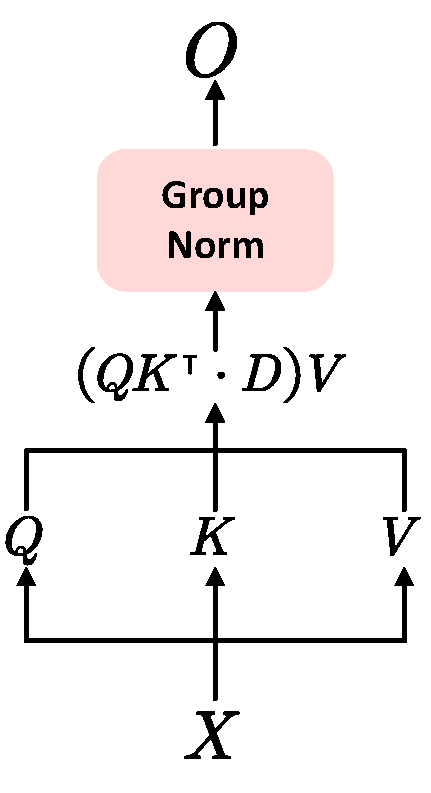
\includegraphics[width=\linewidth]{Img/并行计算过程.pdf}
        \caption{并行计算过程}
        \label{fig:4-3_a}
    \end{subfigure}
    \begin{subfigure}[b]{0.58\textwidth}
        \centering
        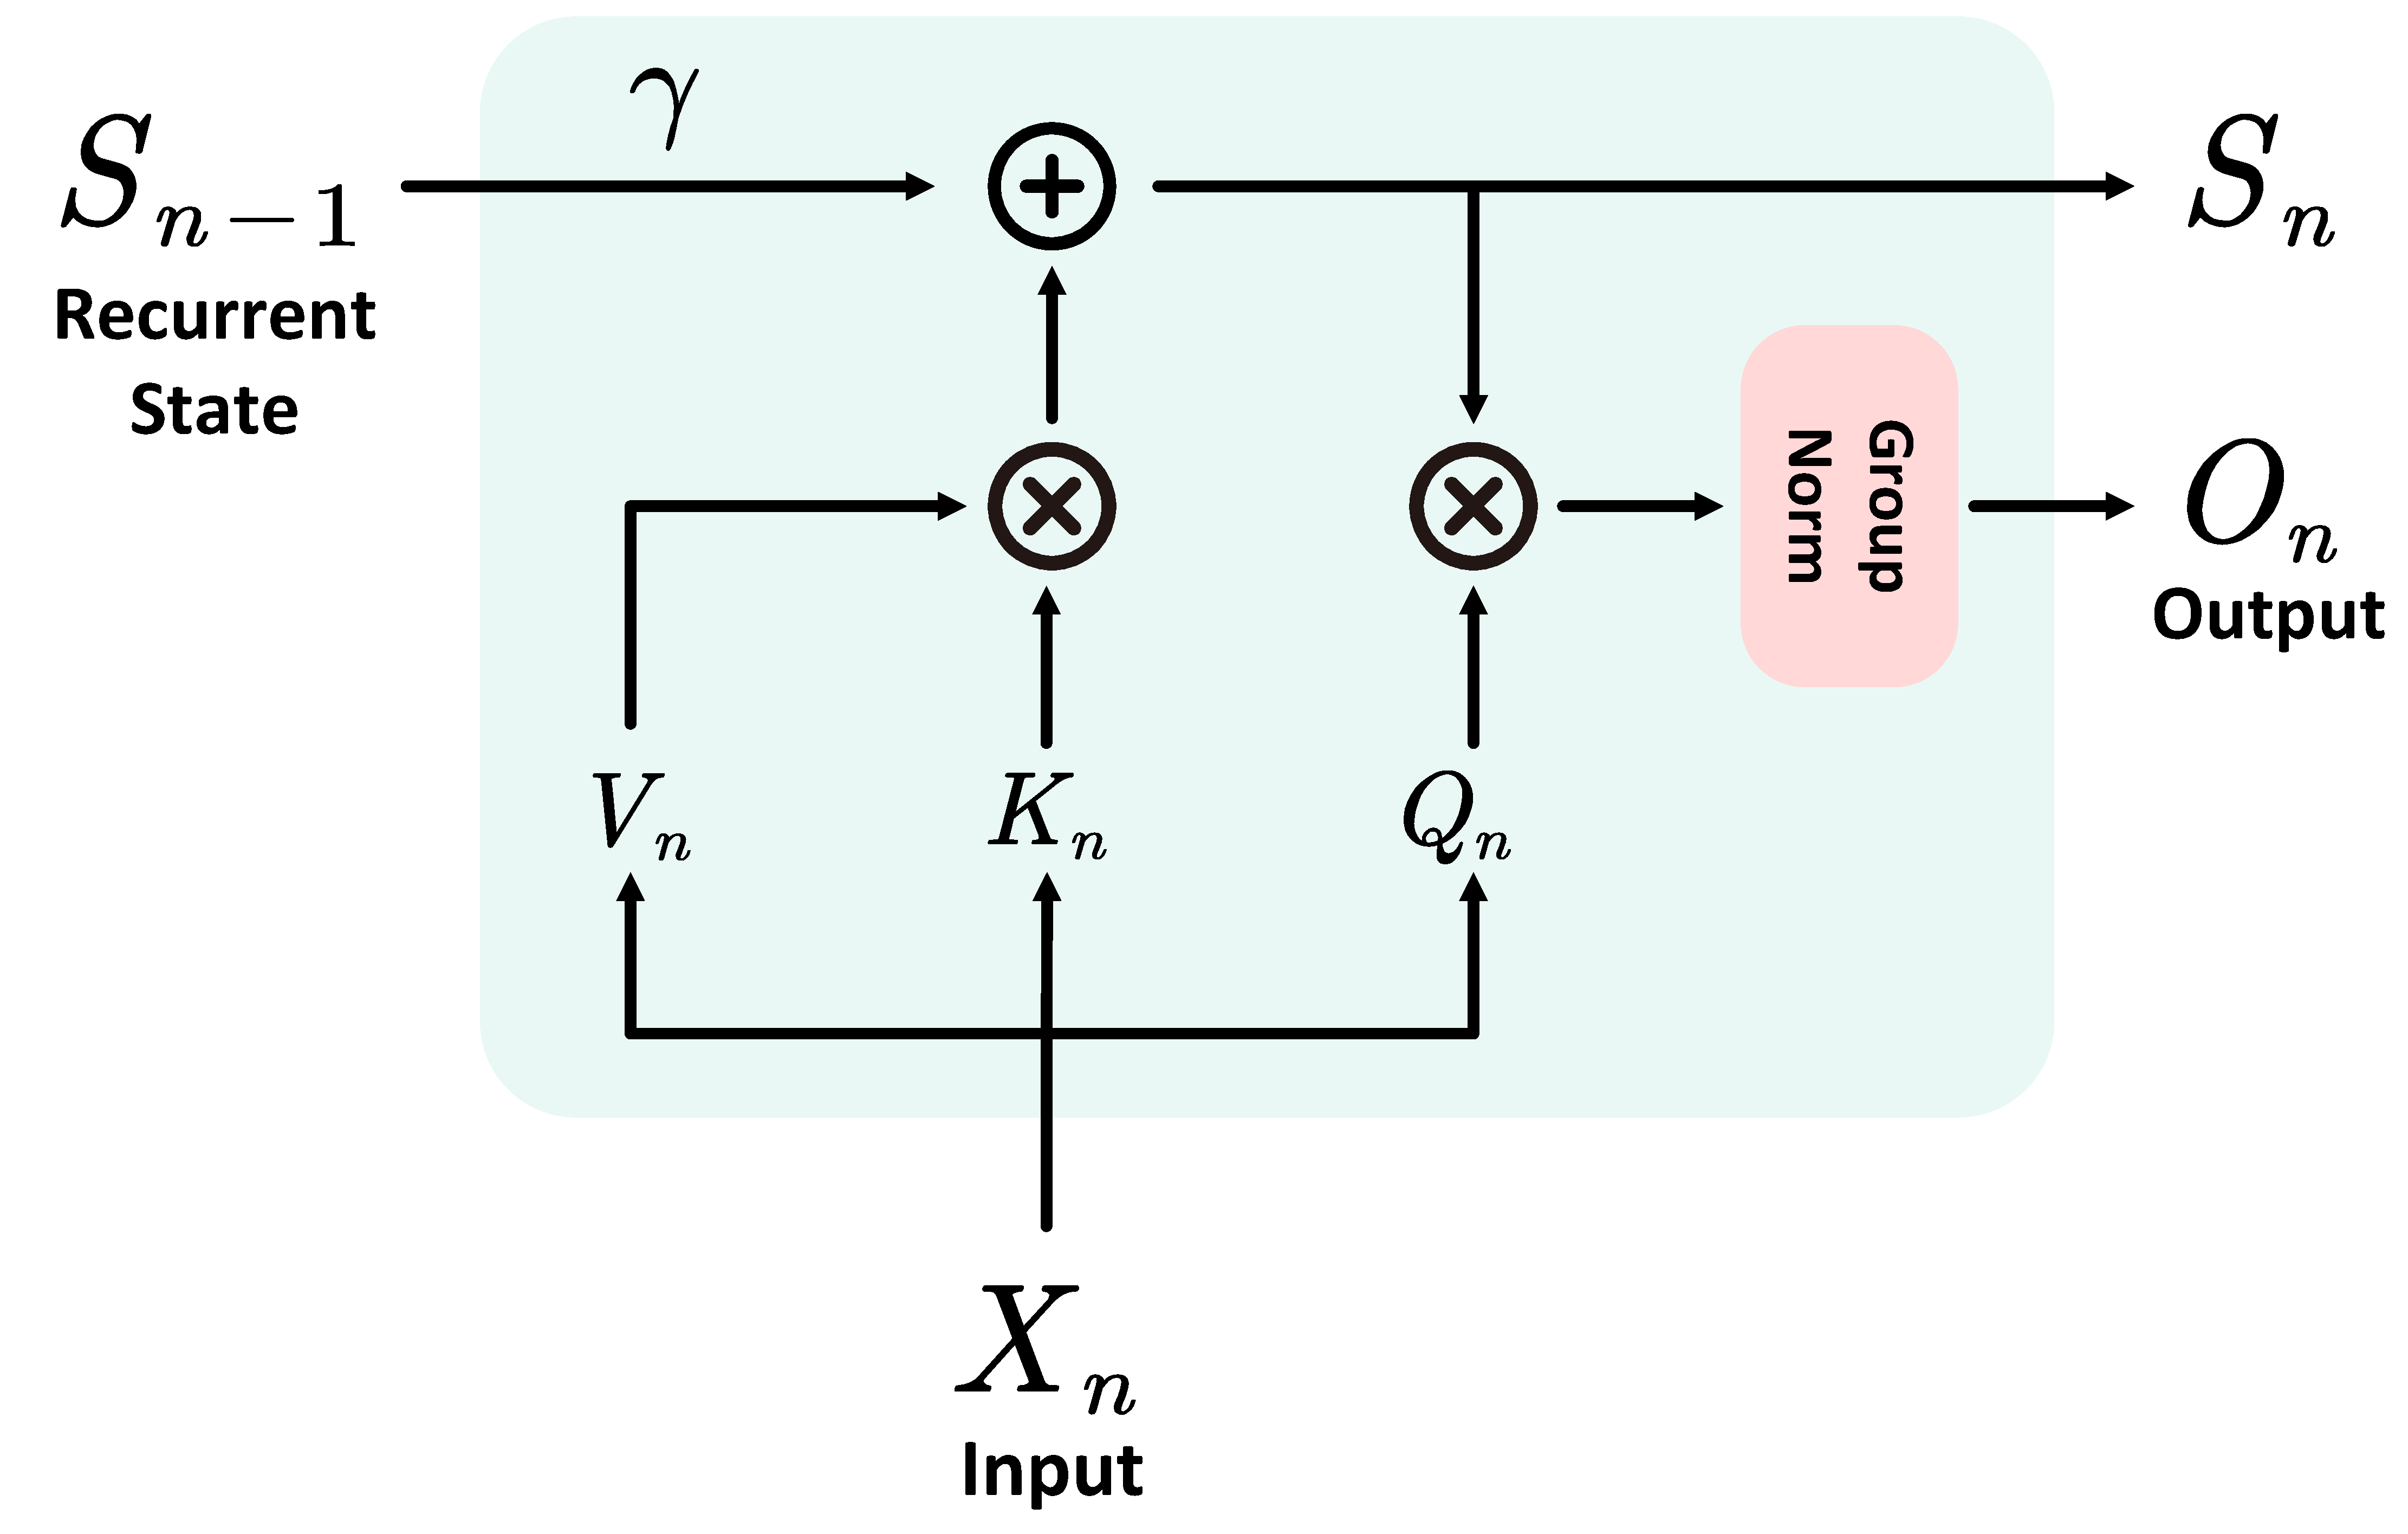
\includegraphics[width=\linewidth]{Img/循环计算过程.pdf}
        \caption{循环计算过程}
        \label{fig:4-3_b}
    \end{subfigure}
    \caption{RetNet的循环化和并行化双重计算过程}\label{fig:4-3}
\end{figure}


经过处理得到的 $X\in\mathbb{R}^{|x|\times d_{\mathrm{model}}}$,我们将其投影到一维的函数 $v(n)=X_n\cdot  {w}_V$,在此过程中,RetNet 设计了一个循环化和并行双重计算过程,如图 \ref{fig:4-3} 所示,使得 $v(n)$ 经过中间状态 $s_n$ 得到输出 $o(n)$,具体的循环计算公式如下:
\begin{align}
    s_n &=As_{n-1}+K_n^\intercal v_n, \quad A\in\mathbb R^{d\times d},K_n\in\mathbb R^{1\times d} \label{eq:4-0}\\
    o_n &=Q_ns_n=\sum_{m=1}^nQ_nA^{n-m}K_m^\intercal v_m, \quad Q_n\in\mathbb R^{1\times d} \label{eq:4-1}
\end{align}

其中的 $v_n$ 和 $o_n$ 即为 $v(n)$ 和 $s(n)$,之后,定义一个可学习的矩阵:$W_Q,W_K\in\mathbb{R}^{d\times d}$,因此,投影 $Q_n$ 和 $K_n$的内容感知如下:
\begin{align}
    Q=XW_Q,\quad K=XW_K
\end{align}

然后对公式 \ref{eq:4-0} 中的 $A$ 矩阵进行奇异值分解操作,得到 $A = \Lambda(\gamma e^{i\theta})\Lambda^{-1}, \gamma,\theta\in\mathbb{R}^d$,同理,对于 $n-m$ 次循环,可以得到 $A^{n-m} = \Lambda(\gamma e^{i\theta})^{n-m}\Lambda^{-1}, \gamma,\theta\in\mathbb{R}^d$,用这个 $A^{n-m}$ 的表达式替换掉公式 \ref{eq:4-1} 中的 $A^{n-m}$,整理后的 $o_n$ 的计算公式如下:
\begin{equation}
    \begin{split}
    o_{n}& =\sum_{m=1}^nQ_n(\gamma e^{i\theta})^{n-m}K_m^\intercal v_m \\
    &=\sum_{m=1}^n(Q_n(\gamma e^{i\theta})^n)(K_m(\gamma e^{i\theta})^{-m})^\intercal v_m \\
    &=\sum_{m=1}^n\gamma^{n-m}(Q_ne^{in\theta})(K_me^{im\theta})^\dagger v_m
    \end{split}
\end{equation}

其中 $\dagger$ 表示共轭转置,之后针对整体的计算过程进行并行化,如图 \ref{fig:4-3_a} 所示,具体的表达式如下所示:
\begin{align}
    Q=(XW_Q)\odot\Theta,\quad K &=(XW_K)\odot\overline{\Theta},\quad V=XW_V\\
    \Theta_n= e^{in\theta},\quad D_{nm}&=\begin{cases}\gamma^{n-m},&n\geq m\\0,&n<m\end{cases}\\
    \text{Retention}(X) &=(QK^\intercal\odot D)V
\end{align}

\begin{figure}[ht]
  \centering
  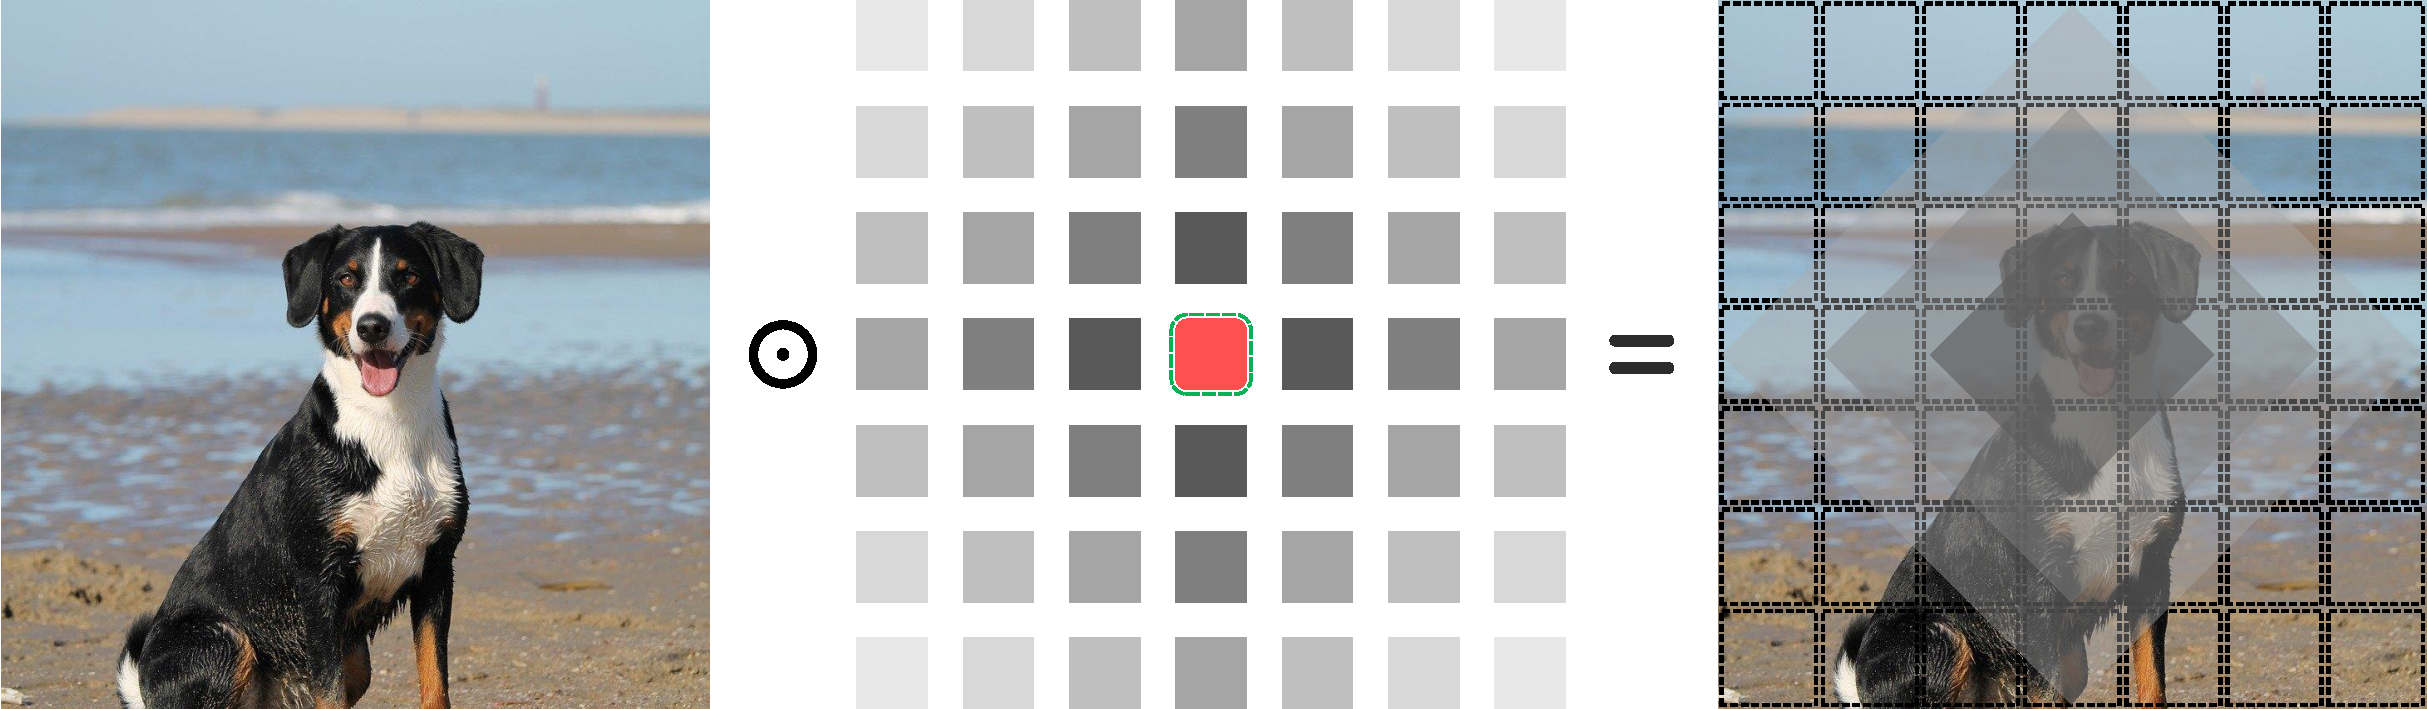
\includegraphics[width=0.9\textwidth]{./Img/空间衰减注意力.pdf}
  \caption{ESD:基于显式超先验的空间衰减注意力}\label{fig:4-5}
\end{figure}


其中 $\overline{\Theta}$ 是 $\Theta$ 的复共轭,$D\in \mathbb{R}^{|x|\times|x|}$ 包含因果掩蔽和指数衰减,它表示一维序列中的相对距离,并带来上下文数据的显式时间先验。受到 RetNet 一维显式时间先验思想的启发,我们创新性的设计了一种基于空间显式超先验的空间衰减注意机制(\textbf{ESD}),如图 \ref{fig:4-5} 所示,在上述并行化计算的基础之上,将其拓展为二维空间衰减注意机制。

在图像的上下文数据中,每个元素标记都通过平面内的二维坐标进行唯一定位,第 $n$ 个标记表示为 $(x_n, y_n)$。 为了适应这一点,需要调整矩阵 $D$ 中的每个元素,以基于其 $2D$ 坐标来表示各个标记对之间的空间相对距离。矩阵 $D$ 的计算公式如下:
\begin{align}
    D_{nm}^{2d}=\gamma^{|x_n-x_m|+|y_n-y_m|}
\end{align}

\begin{figure}[ht]
  \centering
  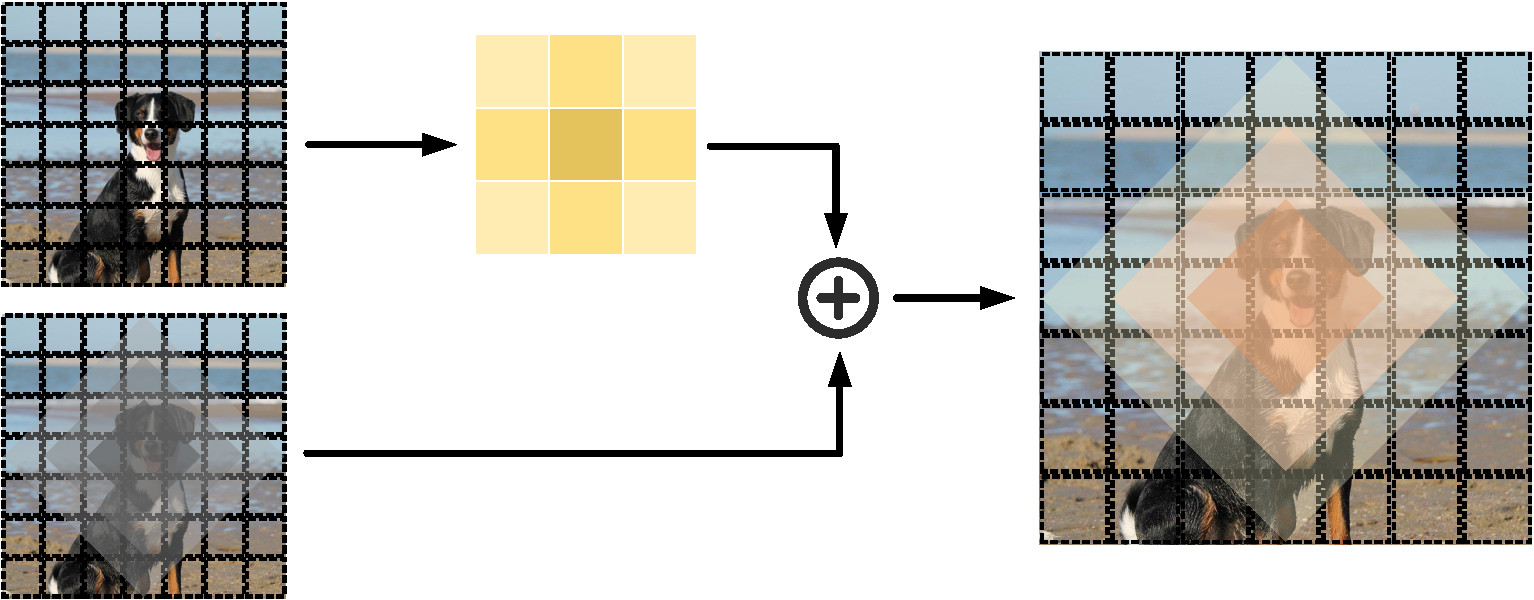
\includegraphics[width=0.876\textwidth]{./Img/输出结合.pdf}
  \caption{空间衰减注意力结合卷积增强得到最终输出}\label{fig:4-6}
\end{figure}


最后,引入 $\text{Softmax}(\cdot)$ 进行非线性操作,再结合上下文增强的卷积操作得到最终的输出,如图 \ref{fig:4-6},因此,完整的空间衰减注意机制的表达式为:
\begin{align}
    \mathrm{ESD}(X)&=(\mathrm{Softmax}(QK^{\mathsf{T}})\odot D^{2d})V\\
    D_{nm}^{2d}&=\gamma^{|x_{n}-x_{m}|+|y_{n}-y_{m}|} \\
    X_{out} &= \mathrm{ESD}(X)+\mathrm{Conv}(V)
\end{align}



\subsubsection{损失函数设计}

在本研究中,我们使用了基于二进制哈希学习的方法对于全局特征和局部特征进行哈希学习。对于 $q$ 个查询数据点,将其表示为 $\{q_i\}_{i=1}^q$,同时,对于 $p$ 个数据点,将其表示为 $\{p_i\}_{i=1}^p$。然后,针对每一对的 $q_i$ 和 $p_j$,将由一个全局特征 $v^{global}$ 和 $m$ 个局部特征 $v^{local}_i$ 组成,每一对的 $q_i$ 和 $p_j$ 对应的哈希码可以通过下面公式得到:
\begin{align}
    u_i=\operatorname{sign}(q_i) ,\quad z_j=\operatorname{sign}(p_j)
\end{align}

其中,$u_i,z_j\in\{-1,+1\}^k$,$k$ 代表着最终输出的二进制哈希码的长度。设 $F$ 表示模型中全局和局部特征学习的整合,$\mathrm{W}=\{\mathrm{W}^{global};\mathrm{W}_1^{local};\mathrm{W}_2^{local};\ldots;\mathrm{W}_m^{local}\}$为二进制代码映射模块,$\Theta$ 代表模型需学习的参数集。对于给定的输入图像 $I$,全局和局部特征学习整体输出如下:
\begin{align}
    O = \mathrm{W} \cdot F(I;\Theta)
\end{align}

然后,我们使用 $\text{tanh}(\cdot)$ 针对 $O$ 进行激活得到模型最终的输出 $O^\prime = \text{tanh}(O)$,最终的损失 $\mathcal{L}$ 设计如下:
\begin{align}
    \mathcal{L}_{\mathrm{W},\Theta}(I)=
        \alpha\sum_{i\in\Omega}\sum_{j\in\Gamma}\left[{O^\prime_i}^\top z_j-kS_{ij}\right]^2+\beta\sum_{i\in\Omega}\left[z_i-{O^\prime_i}\right]^2
    \label{eq:final_eq}
\end{align}

其中 $\alpha$ 和 $\beta$为网络训练时的权衡超参数,$\Gamma$ 代表所有数据库点的索引,而 $\Omega \subseteq \Gamma$ 表示查询集点的索引。$S \in \{-1,+1\}{}^{q \times p}$ 是一个监督矩阵,其值可以在模型训练过程中自动调整。在 LGESD 模型中,我们规定在每次计算损失时,数据库点与查询集点之间不能有共同的项,确保数据库和查询集之间保持互补关系。

\subsubsection{实验过程设计}

\textbf{数据集划分}:本研究在四个数据集上进行,分别是CUB200-2011 \cite{Wah2011TheCB}、Aircraft \cite{maji2013finegrained}、Food101 \cite{food101_2014} 以及 NABirds \cite{nabirds2015},其中 CUB200-2011 和 Aircraft 属于广泛使用的数据集,Food101 和 NABirds 属于流行的大规模细粒度数据集。CUB200-2011 为鸟类数据集,包含了200种鸟类的11788张图像,我们将其分为5994张图像用于训练,5794张图像用于测试。Aircraft 为飞机数据集,包含了100种类型飞机的10000张图像,将其中6667张图像用于训练,3333张图像用于测试。Food101 为具有101000张图像的101种食品类数据集,每个类别中有1000张图像,我们按照每个类别挑选750张图像用于训练,250张用于测试,划分出训练图像75750张,测试图像25250张。NABirds 包含了48562张图像的北美鸟类数据集,其中555种北美子鸟类,我们将23929张图像用于训练,24633种图像用于测试。


\textbf{训练设置}:对于CUB200-2011、Aircraft 以及 Food101 三个数据集,我们设置每个 Epoch 随机采样的样本数为2000个,而对于 NABirds 数据集,设置每个 Epoch 随机采样的样本数为 4000 个。对于所有的数据集,我们设定每张输入的图像预处理为 $224 \times 224$ 大小,训练次数 Epoch 为30次,设定迭代时间为 50,迭代的学习率设置为 $5 \times 10^{-4}$,批量的大小设置为 16,使用 SGD 作为优化器,骨干网络选择 ResNet-50 \cite{he2015deep},训练过程的权重衰减和动量分别设置为 $10^{-4}$ 和 $0.91$。在公式 \ref{eq:final_eq} 中的 $\alpha$ 和 $\beta$ 我们分别设置为 $0.6$ 和 $30$。在公式 \ref{eq:eq_4_m} 中的 $m$ 我们设置为3,因此最终的全局和局部双轨结构的输出哈希码长度分别为 $\frac{k}{2}$ 和 $\frac{k}{6}$,其中 $k$ 为训练时指定的最终输出的哈希码的长度。


\begin{figure}[h]
  \centering
  \begin{subfigure}{0.48\textwidth}
    \centering
    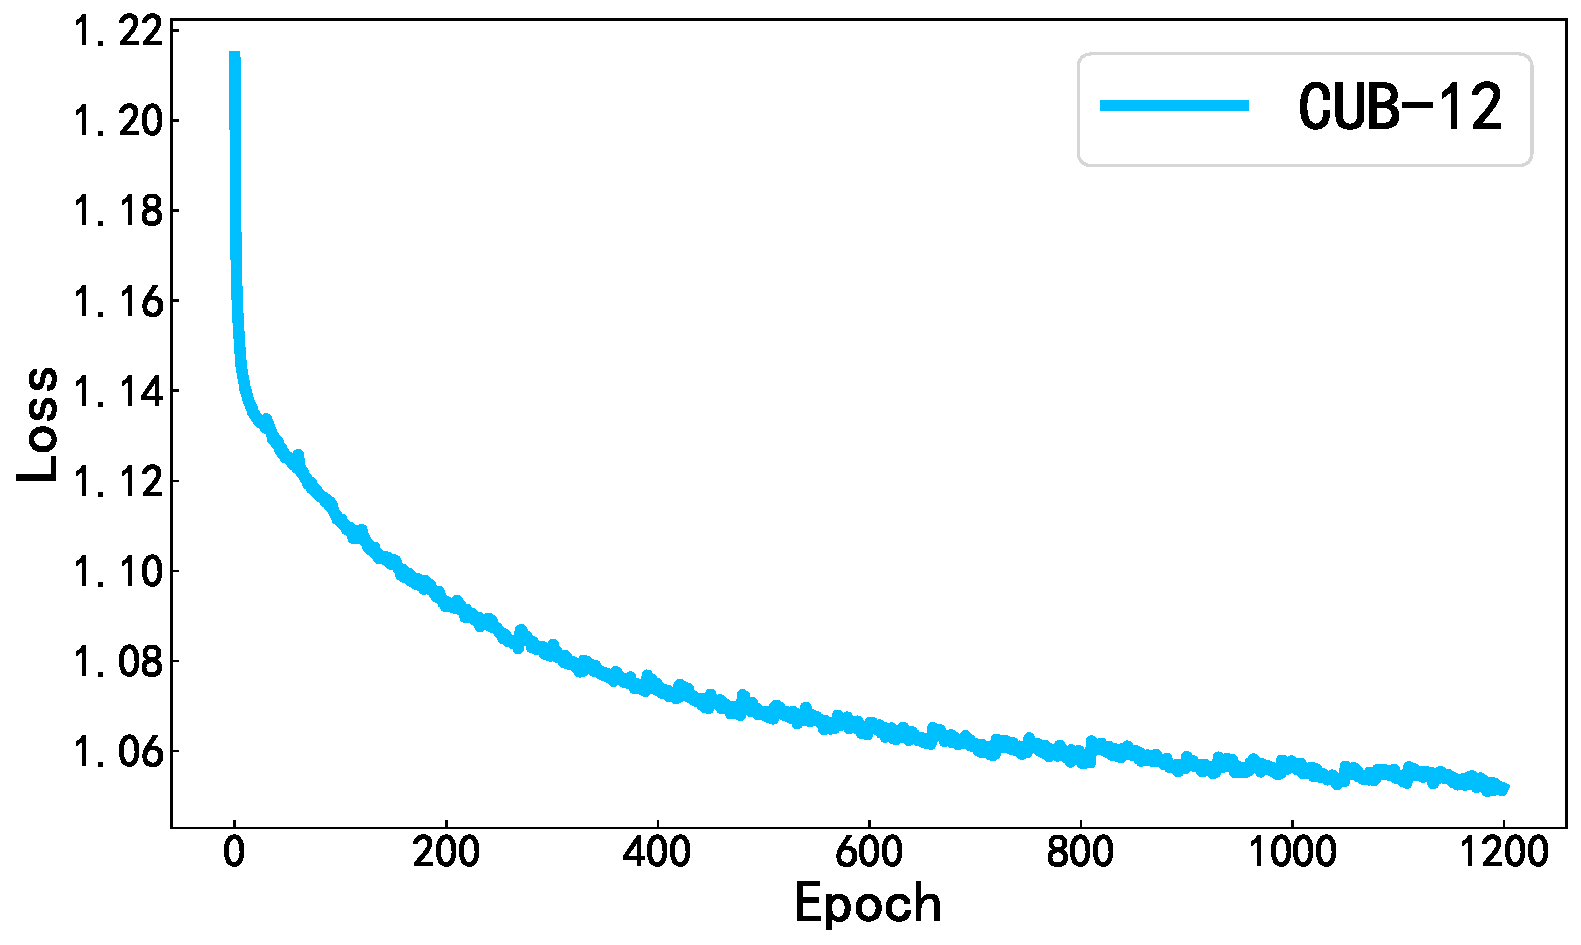
\includegraphics[width=\linewidth]{./Img/CUB-12.pdf}
    \caption{$k=12$}\label{fig:4-24}
  \end{subfigure}
  \hfil
  \begin{subfigure}{0.48\textwidth}
    \centering
    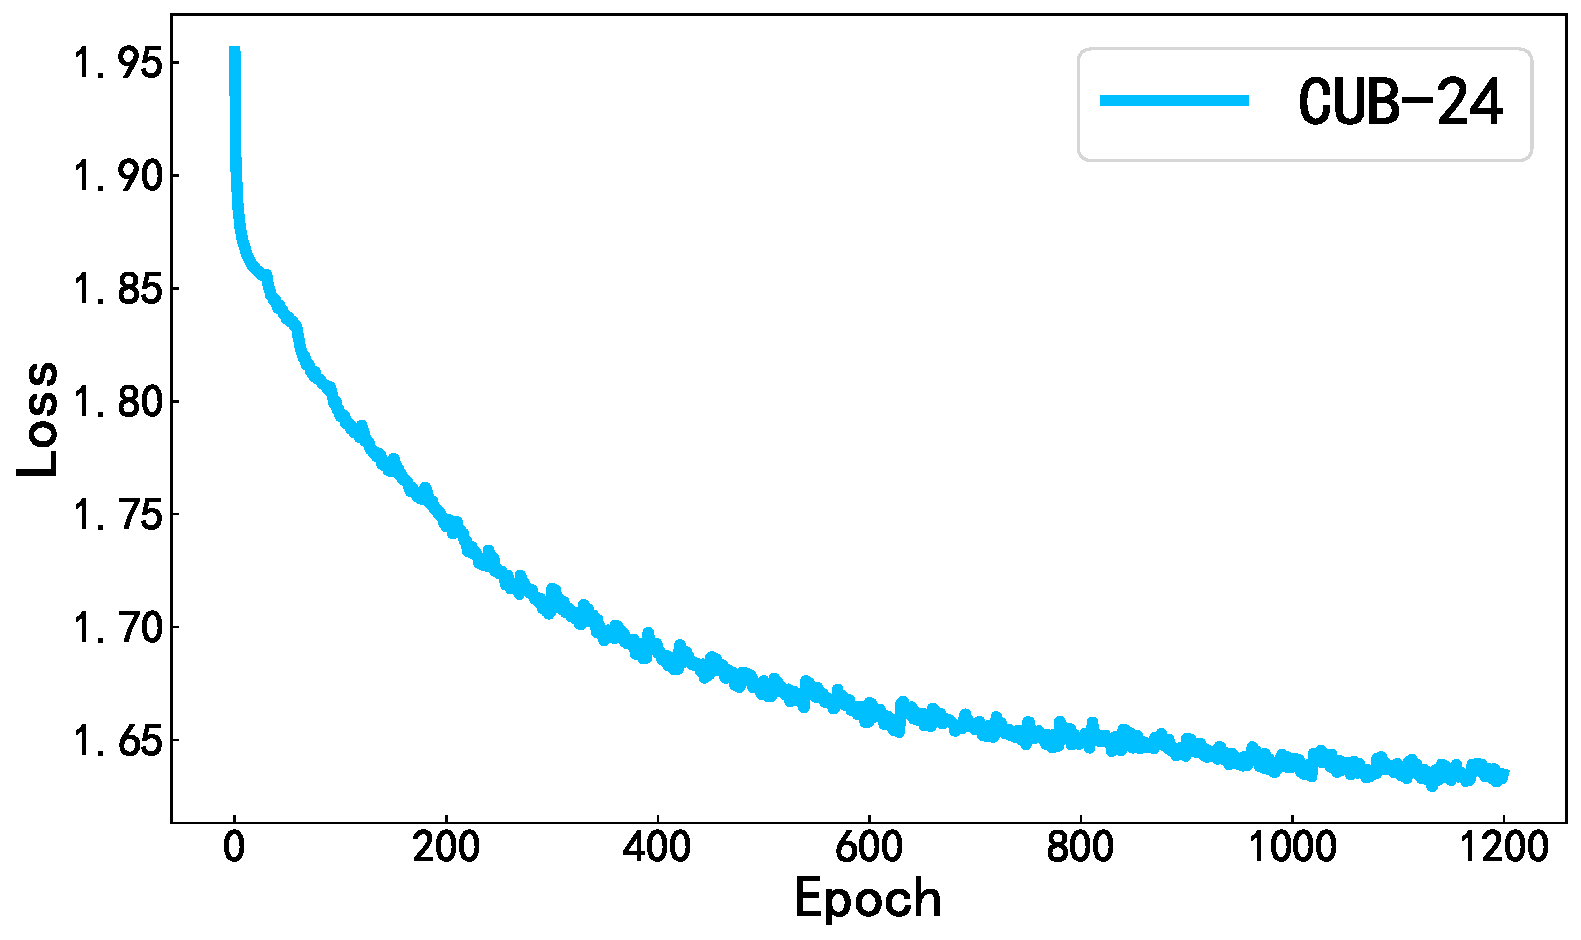
\includegraphics[width=\linewidth]{./Img/CUB-24.pdf}
    \caption{$k=24$}\label{fig:4-25}
  \end{subfigure}
  \hfill
  \begin{subfigure}{0.48\textwidth}
    \centering
    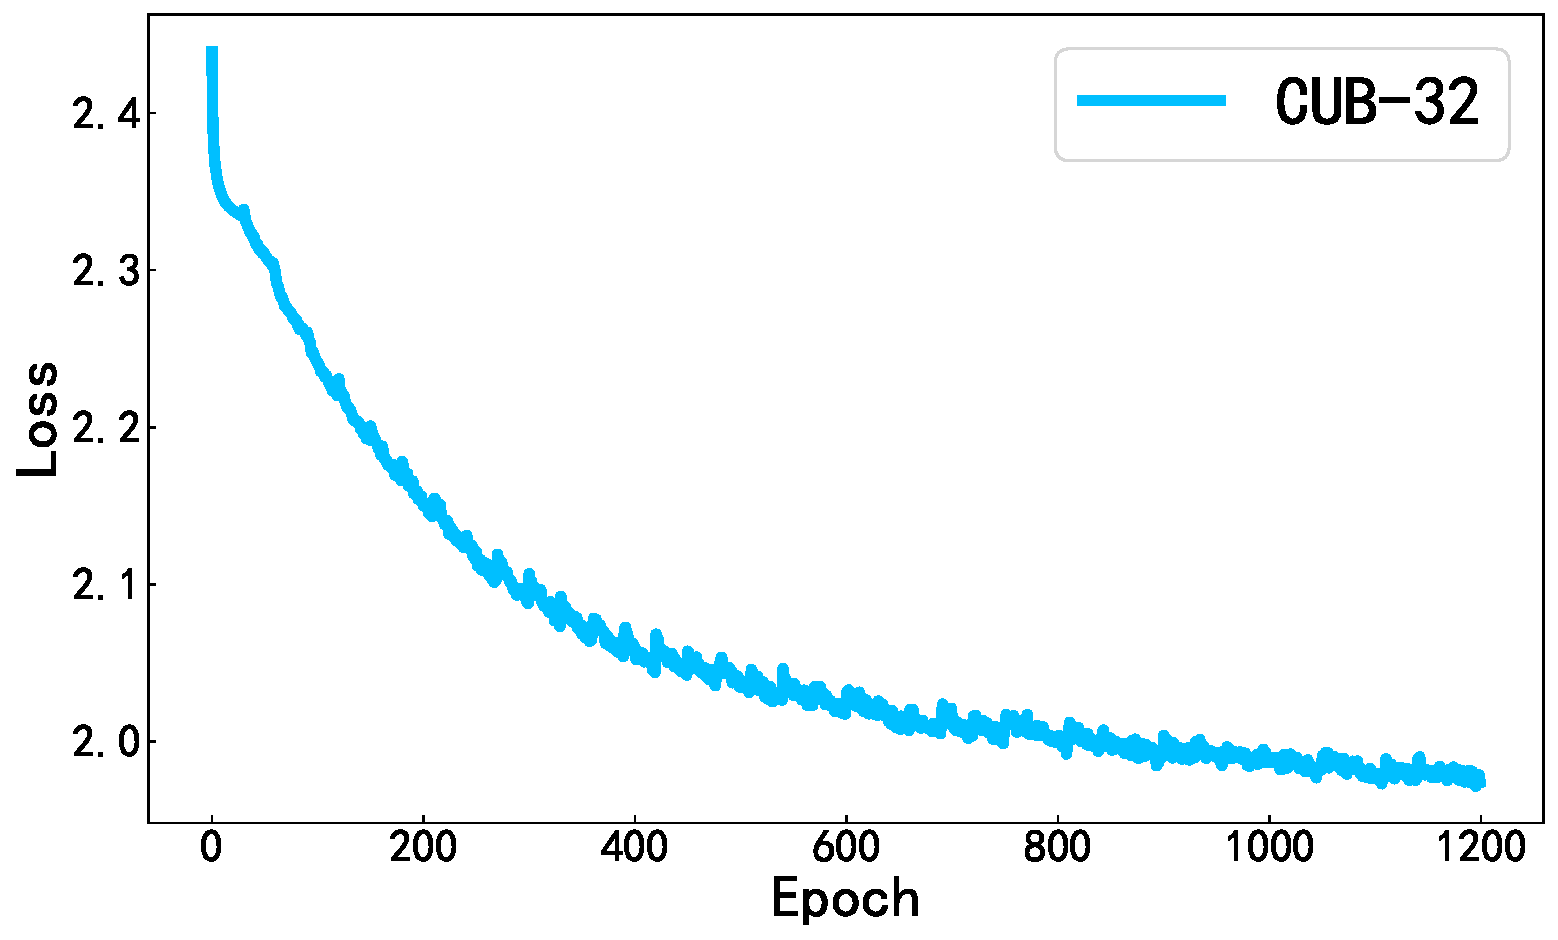
\includegraphics[width=\linewidth]{./Img/CUB-32.pdf}
    \caption{$k=32$}\label{fig:4-26}
  \end{subfigure}
  \hfil
  \begin{subfigure}{0.48\textwidth}
    \centering
    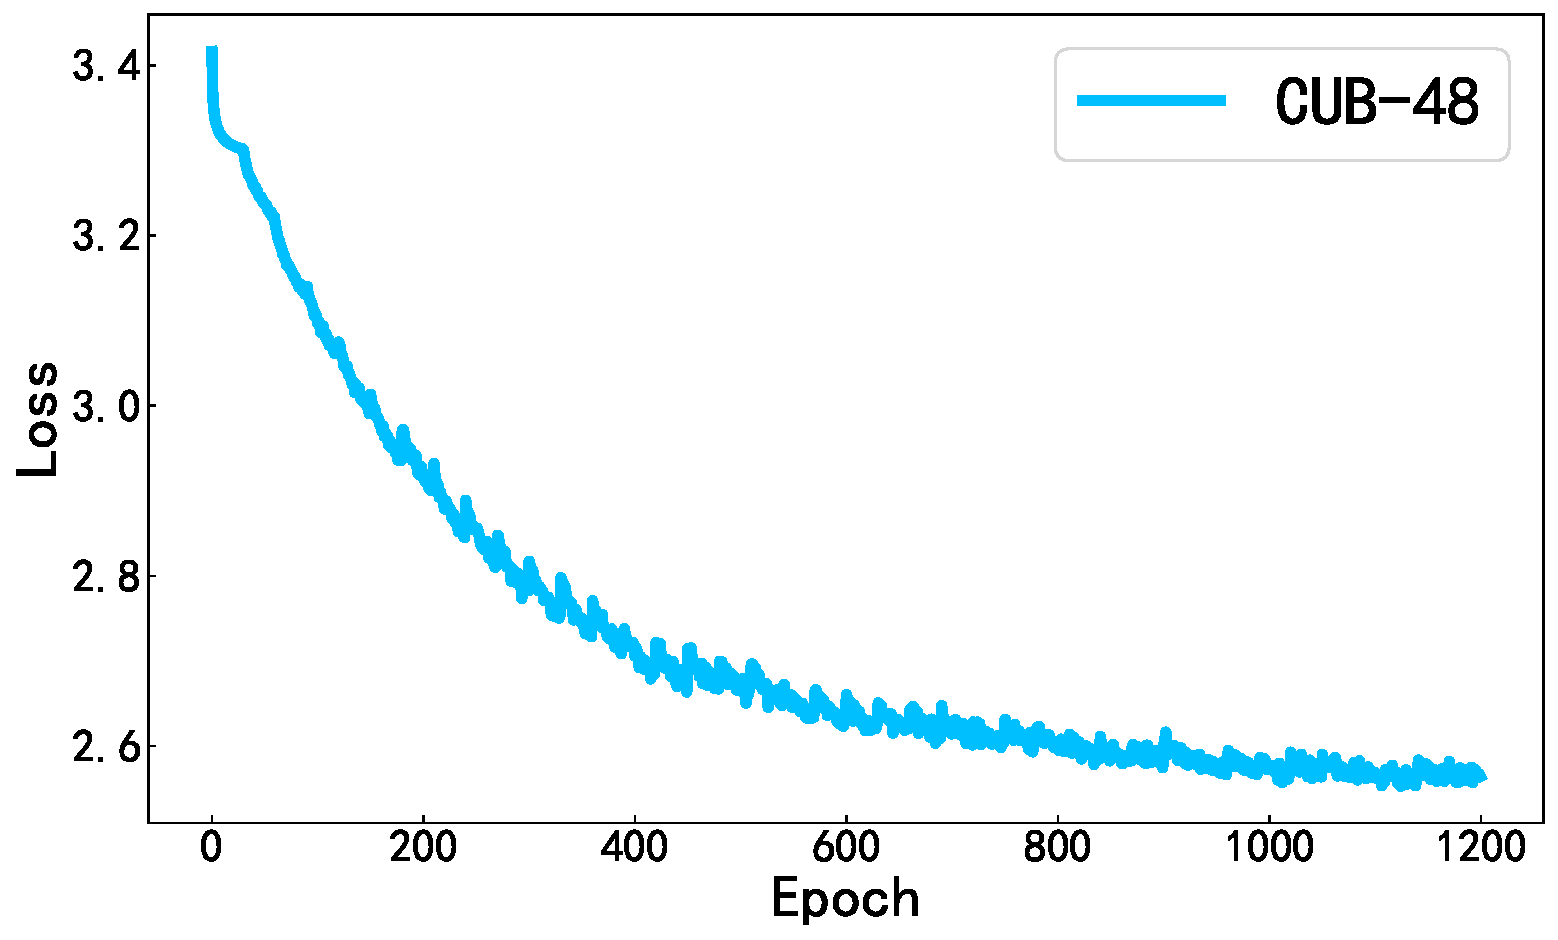
\includegraphics[width=\linewidth]{./Img/CUB-48.pdf}
    \caption{$k=48$}\label{fig:4-27}
  \end{subfigure}
  \caption{CUB200-2011数据集的12-48哈希码长度训练损失}
  \label{fig:4-28-a}
\end{figure}

如图 \ref{fig:4-24} 至 \ref{fig:4-27} 所示,这一系列四幅图表详尽描绘了LGESD在同个数据集的不同哈希码长度上的训练进程中,损失函数的演变轨迹。当哈希码长度为32时,损失值从初始的2.4稳步下探至约2.0,直观展示了模型效能的稳步提升。类似地,哈希码长度为12的训练轨迹亦呈现出乐观的下降态势,损失值由1.22优化至1.06,再度验证了模型在迭代学习中的持续优化能力。在采用48位哈希码的配置下,因编码长度的增益,模型被赋予了学习更为复杂和丰富的特征表达空间的能力,进而导致初期损失值设定于较高水平(3.0)。然而,随着训练进程的推移,这一数值稳步下滑至约2.6,并呈现平稳趋势,这一动态不仅揭示了模型在克服初期高挑战起点时的韧性,还显著证明了其在应对高级分类任务时的学习效率与灵活适应性。综观所有实验情境,随着训练次数(Epoch)的累加,损失函数的递减速率渐趋缓慢,标志着模型学习已逼近收敛状态,实现了训练目标。

\begin{table*}[h]
	\caption{LGESD模型的平均预测精度(\%mAP)与现有方法对比}
	\label{tab:experiments}
	\centering
	\resizebox{1.0\linewidth}{!}{
	\begin{tabular}{c|c|cccccccccc}
		\toprule
		数据集 & 哈希码长度 & ITQ & SDH & DPSH & HashNet & ADSH & ExchNet & A${}^2$-Net & \textbf{LGESD}\\		
		\midrule
		\multirow{4}{*}{CUB200-2011}
            &$k=12$&6.80&10.52&8.68&12.03&20.03&25.14&33.83     &  \textbf{41.50}   \\
            &$k=24$&9.42&16.95&12.51&17.77&50.33&58.98&61.01    &  \textbf{67.33}   \\
            &$k=32$&11.19&20.43&12.74&19.93&61.68&67.74&71.61   &  \textbf{74.01}   \\
            &$k=48$&12.45&22.23&15.58&22.13&65.43&71.05&77.33   &  \textbf{80.12}   \\
		\hline
    	\multirow{4}{*}{Aircraft}  
            &$k=12$&4.38&4.89&8.74&14.91&15.54&33.27&42.72      &  \textbf{50.37}   \\
            &$k=24$&5.28&6.36&10.87&17.75&23.09&45.83&63.66     &  \textbf{76.61}   \\
            &$k=32$&5.82&6.90&13.54&19.42&30.37&51.83&72.51     &  \textbf{81.49}   \\
            &$k=48$&6.05&7.65&13.94&20.32&50.65&59.05&81.37     &  \textbf{85.06}   \\
		\hline
		\multirow{4}{*}{Food101}          
            &$k=12$&6.46&10.21&11.82&24.42&35.64&45.63&46.44    &  \textbf{52.16}   \\
            &$k=24$&8.20&11.44&13.05&34.48&40.93&55.48&66.87    &  \textbf{77.71}   \\
            &$k=32$&9.70&13.36&16.41&35.90&42.89&56.39&74.27    &  \textbf{81.05}   \\
            &$k=48$&10.07&15.55&20.06&39.65&48.81&64.19&82.13   &  \textbf{83.20}   \\
		\hline
		\multirow{4}{*}{NABirds}           
            &$k=12$&2.53&3.10&2.17&2.34&2.53&5.22&8.20          &  \textbf{8.96}    \\
            &$k=24$&4.22&6.72&4.08&3.29&8.23&15.69&19.15        &  \textbf{21.34}   \\
            &$k=32$&5.38&8.86&3.61&4.52&14.71&21.94&24.41       &  \textbf{28.64}   \\
            &$k=48$&6.10&10.38&3.20&4.97&25.34&34.81&35.64      &  \textbf{41.88}   \\
		\bottomrule
	\end{tabular}}
\end{table*}


模型训练完成之后,我们针对模型进行平均预测精度(mAP)评估,得到的结果如表 \ref{tab:experiments} 所示,在对四个关键数据集的深入剖析中,LGESD展示出相对于A${}^2$-Net持续且明显的优越性。具体到CUB200-2011数据集,LGESD从采用12位哈希码起始,即以41.50\%的mAP成绩奠定了领先地位,此时A${}^2$-Net为33.83\%;而随着哈希长度扩展至48位,LGESD的mAP显著跃升至80.12\%,与A${}^2$-Net的77.33\%形成对比,进一步凸显其优势。转观Aircraft数据集,这种优势在12至32位的哈希码范围内尤为突出,LGESD从50.37\%逐步攀高至85.06\%的峰值,相比之下,A${}^2$-Net在同一区间的表现由42.72\%增长至81.37\%,虽有进步,但仍略逊一筹。在food101与NABirds这两个数据集的探索中,无论哈希长度如何变化,LGESD均稳固保持其领先地位,不断验证其在多样化任务中的高效性能与适应力。





\subsubsection{实验结果分析}

\begin{figure}[h]
  \centering
  \begin{subfigure}{0.48\textwidth}
    \centering
    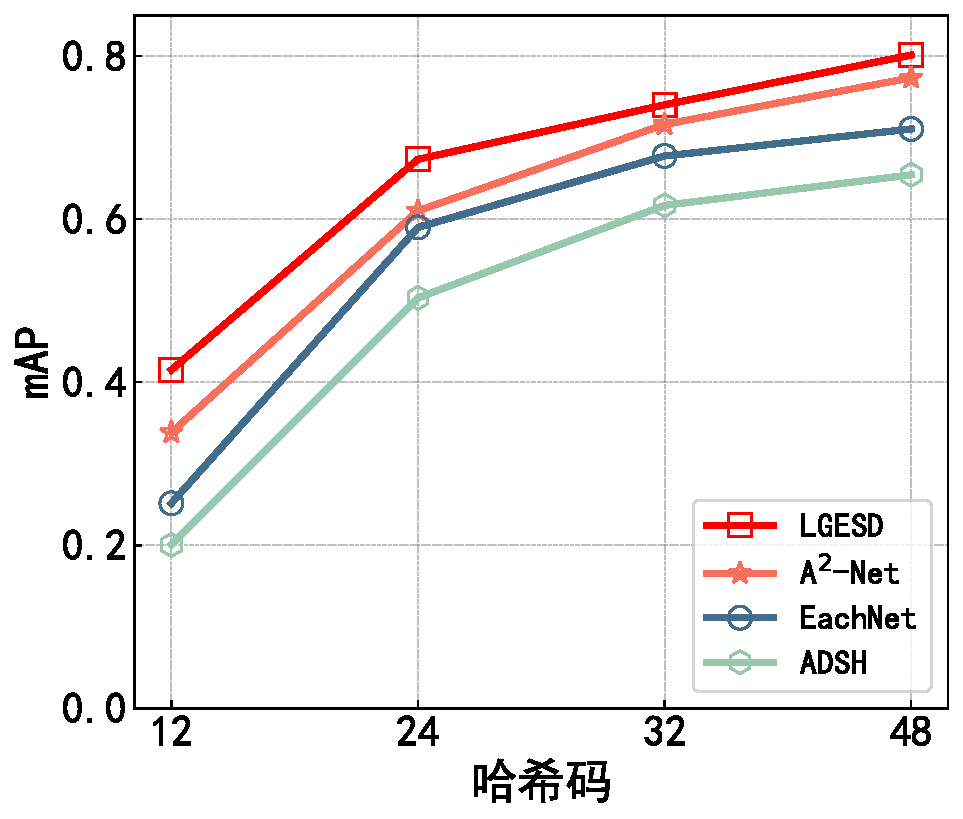
\includegraphics[width=\linewidth]{./Img/CUB-R50.pdf}
    \caption{基于CUB200-2011数据集的mAP对比}\label{fig:4-29}
  \end{subfigure}
  \hfil
  \begin{subfigure}{0.48\textwidth}
    \centering
    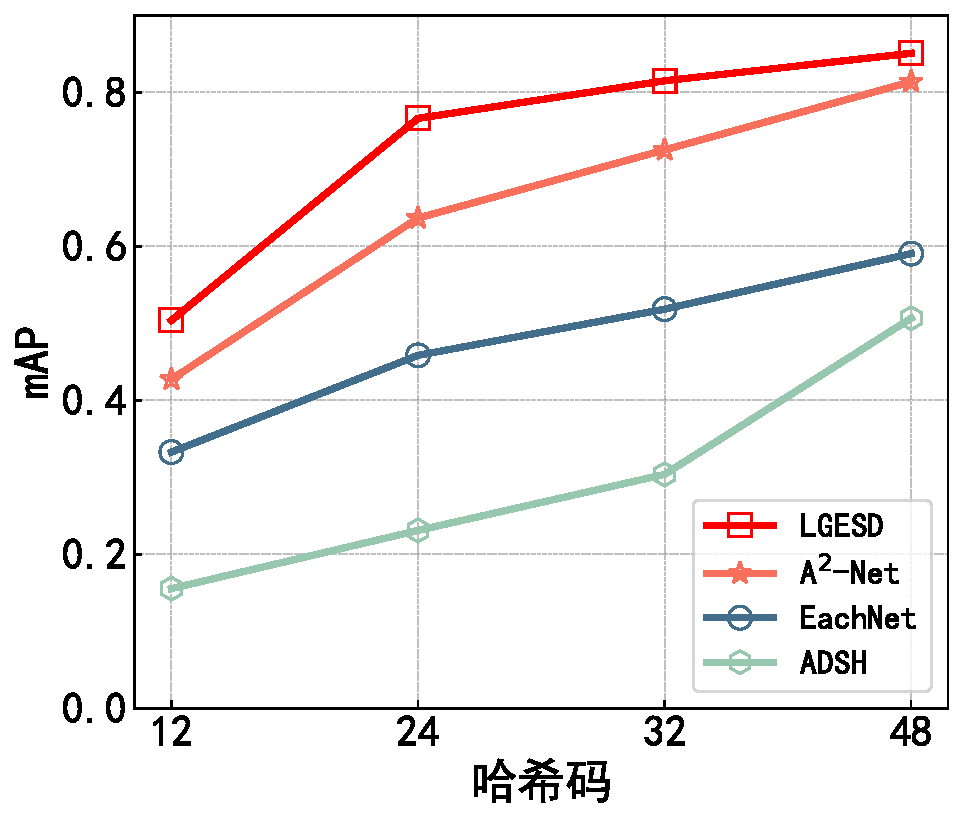
\includegraphics[width=\linewidth]{./Img/Aircraft-R50.pdf}
    \caption{基于Aircraft数据集的mAP对比}\label{fig:4-30}
  \end{subfigure}
  \hfil
  \begin{subfigure}{0.48\textwidth}
    \centering
    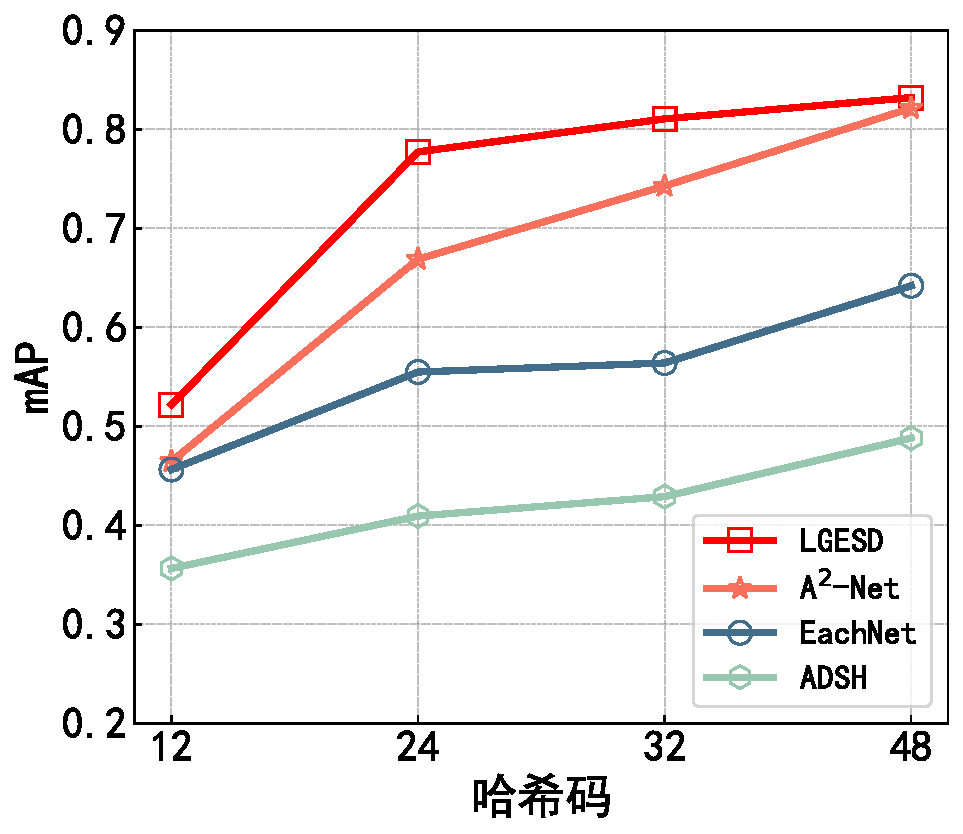
\includegraphics[width=\linewidth]{./Img/Food-R50.pdf}
    \caption{基于Food101数据集的mAP对比}\label{fig:4-31}
  \end{subfigure}
  \hfil
  \begin{subfigure}{0.48\textwidth}
    \centering
    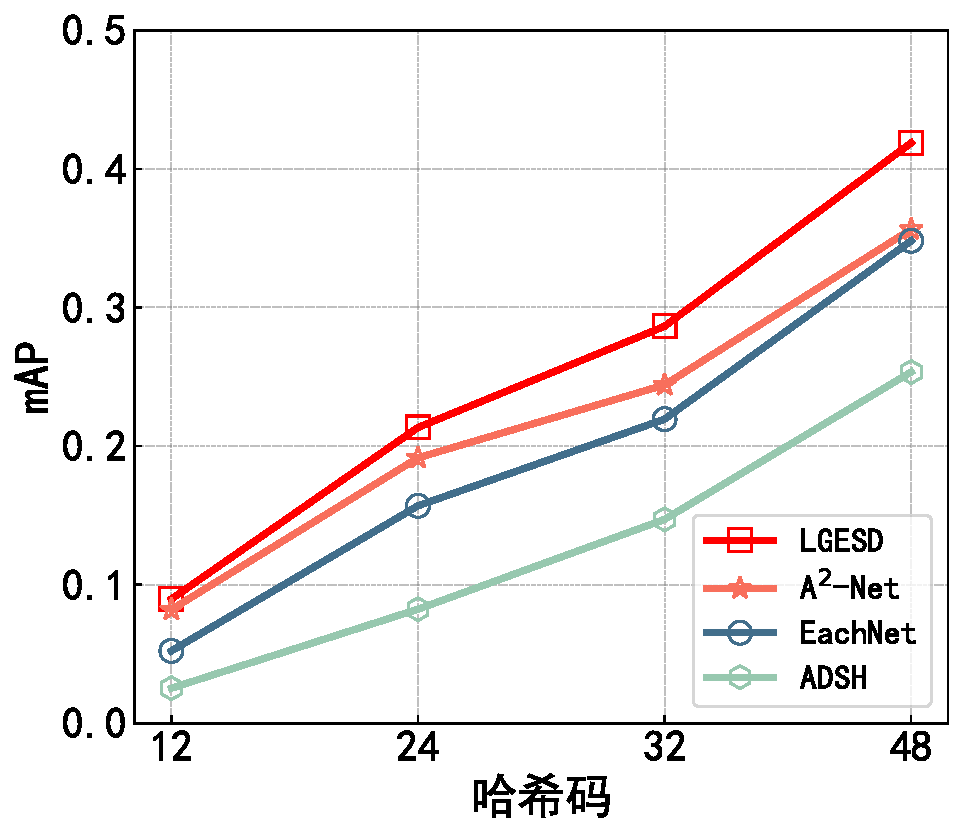
\includegraphics[width=\linewidth]{./Img/Nabirds-R50.pdf}
    \caption{基于NABirds数据集的mAP对比}\label{fig:4-32}
  \end{subfigure}
  \caption{LGESD与现有方法在四个数据集上的mAP对比}
  \label{fig:4-32-a}
\end{figure}

为了更清晰的显示LGESD模型较现有方法的mAP提升,我们选择了 LGESD、A${}^2$-Net、EachNet以及ADSH四个方法的12-48哈希码长度进行可视化显示,如图 \ref{fig:4-32-a} 所示,从两个图当中可以看出,LGESD算法模型在哈希码长度变化的影响分析中展现了一种明确的正向发展趋势。随着哈希码长度的逐渐增加,LGESD的平均准确率(mAP)显著提升,这直接反映了哈希码长度与其识别和分类性能之间的正比关系。该特性表明,LGESD算法能够有效利用更长的哈希码来编码更多的输入信息,从而提升其在任务中的表现。这种对哈希码长度增加的敏感性和高效利用,不仅是算法设计合理性的体现,也是其在实践中可能获得更优解的关键因素之一。因此,在资源允许的情况下,针对LGESD模型选择更长的哈希码长度将是一个提升系统性能的有效策略。


\begin{figure}[h]
  \centering
  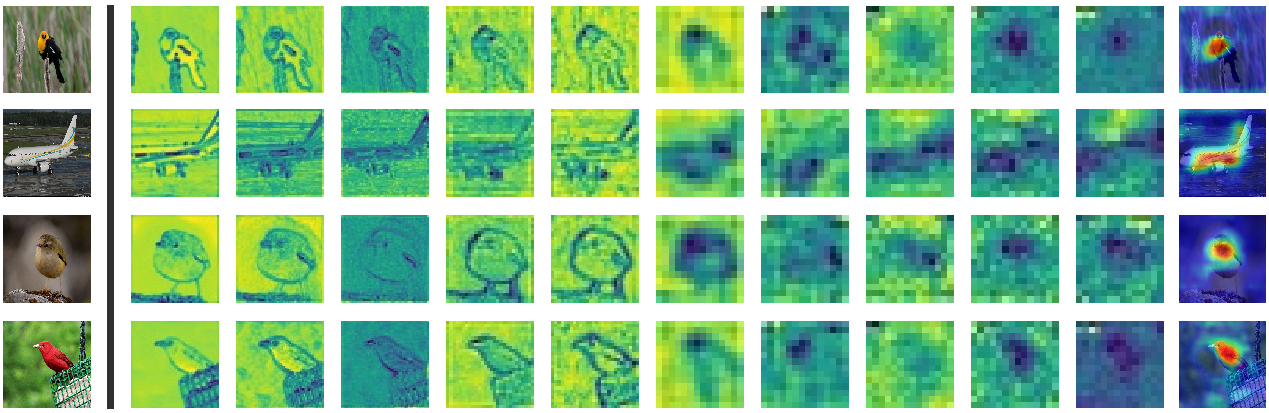
\includegraphics[width=1.0\textwidth]{./Img/中间层特征图.pdf}
  \caption{中间层特征图与注意力热图}\label{fig:4-20}
\end{figure}

图 \ref{fig:4-20} 展示了LGESD模型的训练过程,其中包括输入图像、中间层卷积特征以及注意力热图。从每一行图像的最后一个注意力热图中可以看出,LGESD模型成功地将注意力聚焦在了有效的对象上。这意味着模型能够准确地识别和关注图像中的关键区域,这对于提高模型的性能和准确性非常重要。通过这种集中的注意力,模型能够更好地理解图像内容,并在后续的处理过程中做出更准确的决策。这种成功的注意力聚焦表明模型在训练过程中取得了良好的效果,具备一定的能力处理复杂任务。

\begin{figure}[h]
  \centering
  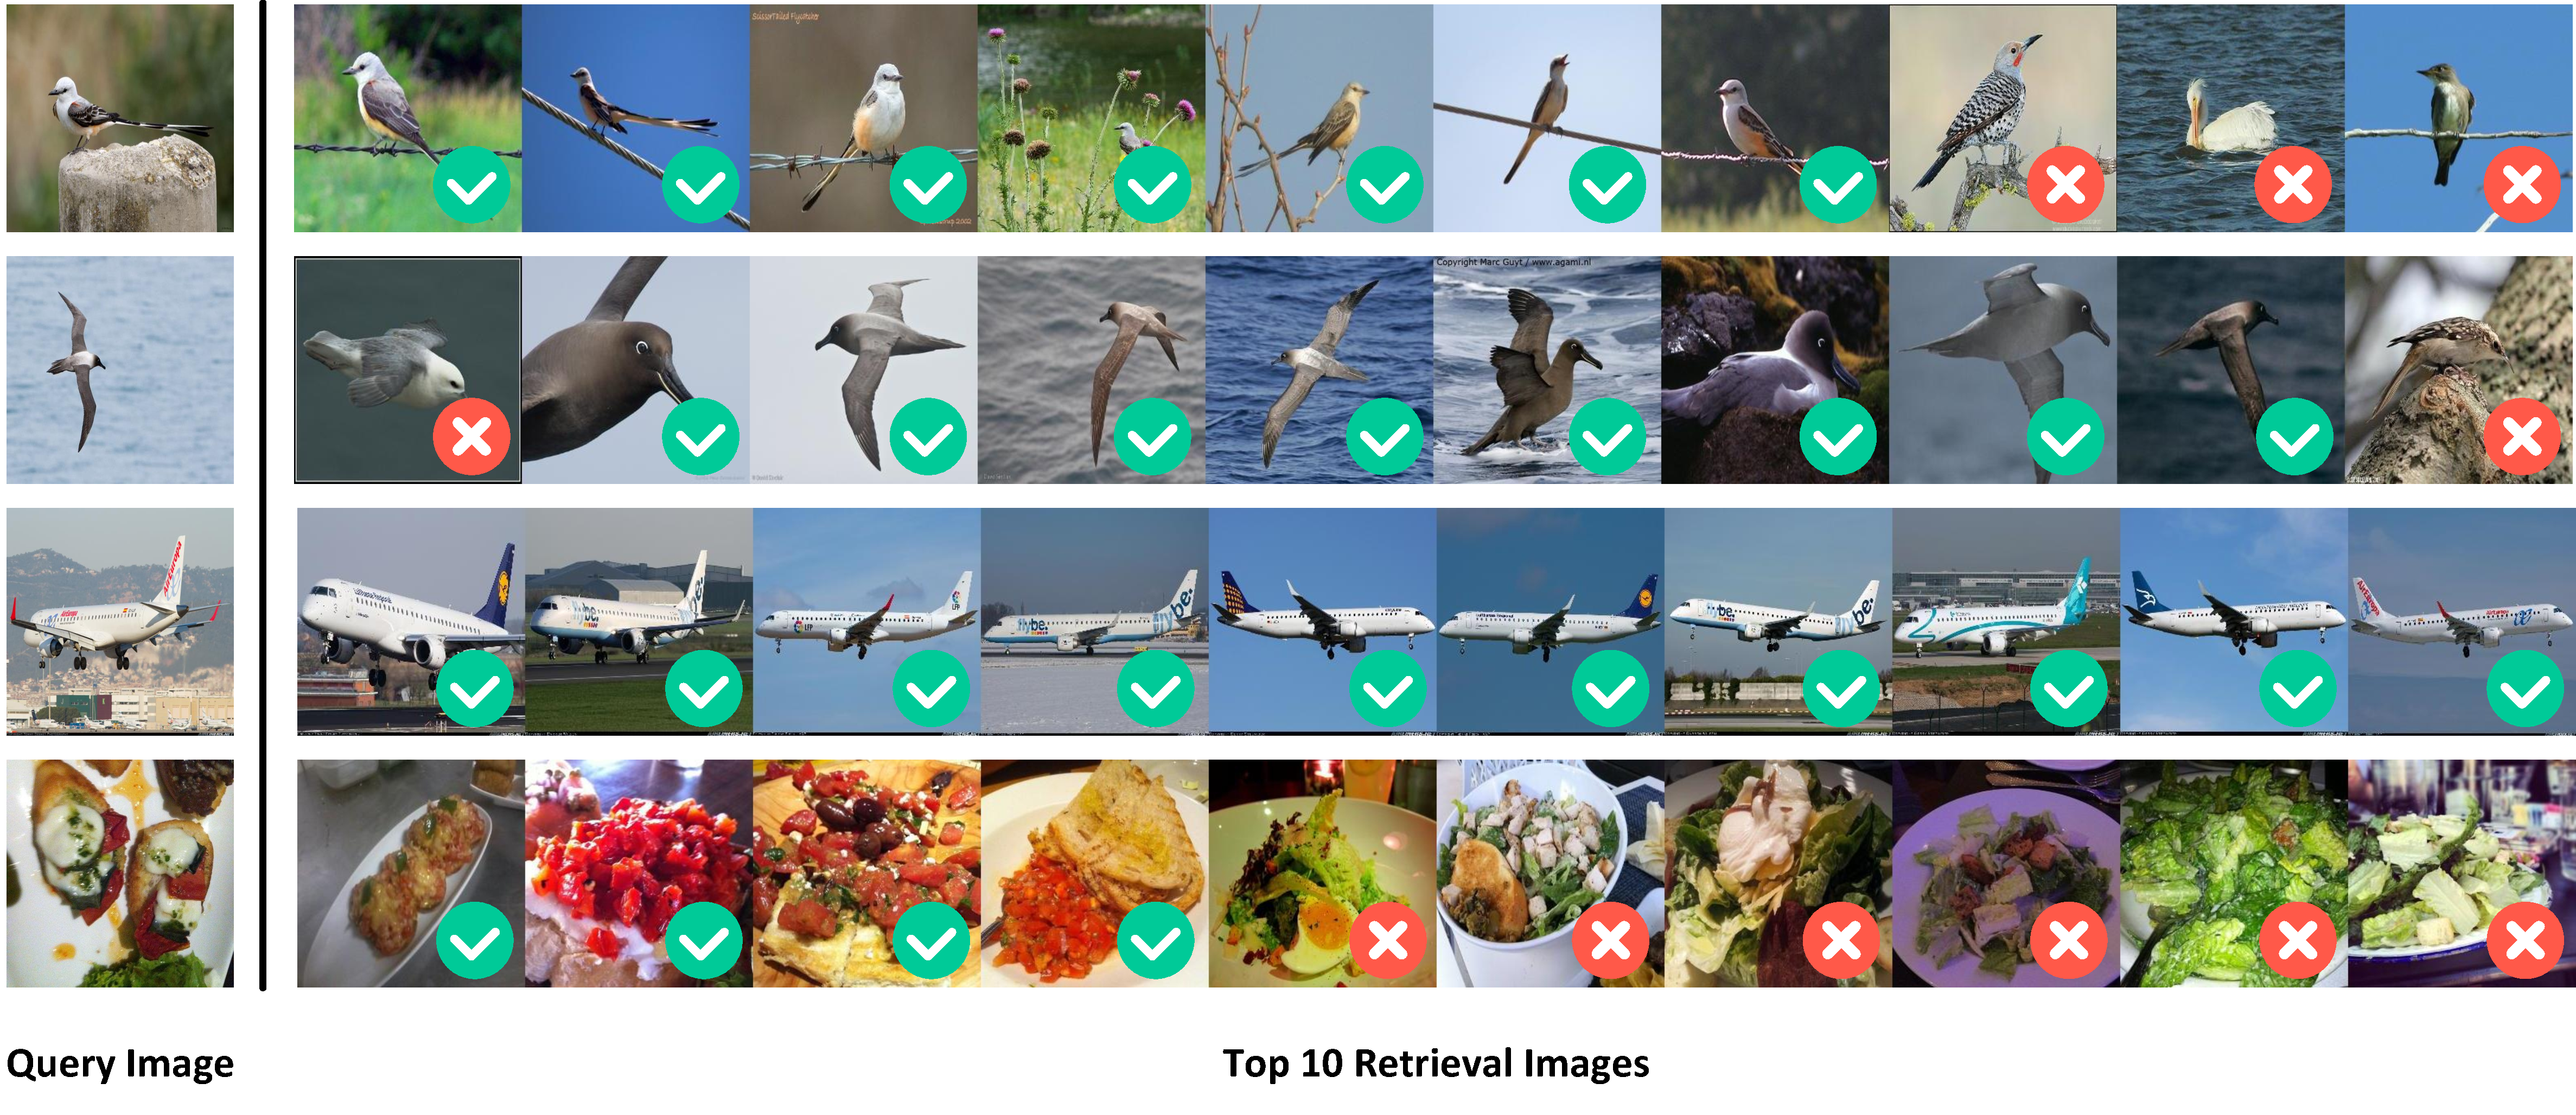
\includegraphics[width=1.0\textwidth]{./Img/最终检索图.pdf}
  \caption{LGESD模型的图像检索效果}\label{fig:4-33}
\end{figure}


在完成模型的训练和损失函数分析之后,我们进一步对模型进行了图像检索能力的测试。测试过程包括随机选取一张未知图像,将其作为查询输入到训练好的模型中。模型基于学习到的特征表示,对数据库中的图像进行排序,以找出与查询图像最相关的图像。我们收集了检索结果中排名最前的前十张图像,并进行了可视化展示。

具体来说,测试中我们首先从图像库中随机抽取了一张未参与训练的图像。随后,该图像被输入至模型,模型随即输出了与其最为相似的一系列图像。这些图像根据与查询图像的相似度得分进行排序,得分最高的图像排在最前。我们选择了排名前十的图像,并将它们与查询图像一起进行了可视化展示,以便于直观评估模型的检索效果,最终得到的可视化结果如图 \ref{fig:4-33} 所示。

在检索结果的前十名中,大多数图像都能正确地识别出与查询图像相同的类别。这一结果表明,模型在图像特征学习和相似性度量方面表现出了较高的准确性和可靠性。然而,尽管前十的检索结果中大部分都正确识别出了对应的类别,但仍有部分图像的识别结果有待提高。这提示我们在未来的工作中需要进一步优化模型的检索性能,可能通过改进特征提取算法、增加训练数据的多样性、调整模型参数等方式来实现。

























\section{研究评价与展望}

\subsection{研究的优势之处}


% 研究角度方面
% 本研究从人工智能与大数据技术在气象预测和图像检索领域的应用出发,提出了两个先进的模型:LSTM长短时记忆网络和LGESD细粒度哈希图像检索模型。这些模型不仅响应了当前技术发展趋势,而且针对特定领域的需求进行了定制化设计,为相关研究领域提供了新的视角和解决方案。

\subsubsection{大数据环境方面}

在大数据时代,本研究提出的模型充分展现了其对海量数据、多样化数据类型以及快速数据更新等挑战的卓越适应性。具体来说,纯LSTM模型和结合CNN的LSTM模型均以其卓越的性能,有效地处理了大规模时间序列数据;而LGESD模型则在大规模图像数据库的快速检索方面表现卓越,两者均展现了出色的可扩展性和适应性。

\subsubsection{模型的可扩展性和泛化能力}

本研究在模型设计时充分考虑了未来的扩展需求,预留了添加新特征和调整模型结构的空间,从而使得模型能够灵活适应更广泛的应用场景。同时在本研究中,LSTM模型、CNN-LSTM模型以及LGESD模型在多个数据集上的稳定表现也证实了其强大的泛化能力。

\subsubsection{框架设计方面}

图 \ref{fig:4-11} 中CNN-LSTM模型的采用延续着时间序列分析领域的一大创新。该模型通过将时间序列数据转换为图像,并运用深度学习技术进行特征提取,有效捕捉了气象数据中的时间序列非线性变化。这种方法在处理气象数据中的长期依赖性问题上取得了显著成效,显著提高了分析的精确度和效率。同时,在图像检索领域,如图 \ref{fig:4-21},LGESD模型引入了显式的空间衰减注意力机制,这一创新技术为细粒度图像检索任务提供了全新的技术手段,一定程度上增强检索的精确度和效率。

\subsubsection{模型评估的全面性}

在本研究中,我们采用了包括均方误差(MSE)、平均绝对百分比误差(MAPE)以及平均预测精度(mAP)在内的多种评估指标,以全面衡量模型的预测性能。这些指标不仅为我们提供了对模型准确性的量化评估,还从不同角度揭示了模型的性能特点。如表 \ref{tab:LSTM_data——pre} 和表 \ref{tab:experiments} 所示,我们详细列出了不同模型在各项评估指标上的具体表现,从而充分展示了本研究所提出模型在多个维度上的优越性。



\subsection{研究的劣势之处}

\subsubsection{数据依赖性}
LSTM模型、CNN-LSTM模型和LGESD模型的表现在很大程度上取决于训练数据的质量和完整性。在现实世界的应用中,为了训练模型,通常需要大量预处理或标注的数据,并且该模型对噪声和异常值具有较高的敏感度。因此,在模型训练过程中,确保数据的准确性和清洁度是至关重要的。

\subsubsection{计算资源}
普遍而言,LSTM模型、CNN-LSTM模型以及LGESD模型在训练和推理阶段可能需要较多的计算资源。在资源受限的情境中,这可能成为限制模型部署和应用的一个因素。因此,在面对有限资源的挑战时,有必要对模型进行优化和简化,以适配可用的计算能力。这可能包括采用更高效的算法、减少模型复杂度、利用模型压缩技术,或是采用分布式计算等策略,以确保模型在资源受限的环境中仍能有效地运行。

\subsubsection{泛化能力的进一步验证}
尽管LSTM模型、CNN-LSTM模型和LGESD模型在多个数据集上已经展现出了良好的性能,但当它们面临与训练数据分布存在显著差异的图像数据时,其泛化能力可能需要进一步的验证和提升。为了确保模型在不同场景下都能保持稳健的表现,有必要通过额外的测试和调整来加强模型对新情况的适应性和灵活性。这可能包括对模型结构的优化、训练策略的改进,或是引入更多样化的训练数据集,以增强模型的泛化能力。



\subsection{研究总结与展望}

\subsubsection{新型的混合模型}

在气象预测领域,我们构建了一种结合卷积神经网络(CNN)和长短时记忆网络(LSTM)的新型混合模型。该模型不仅融合了CNN在特征提取和空间模式识别方面的优势,还利用了LSTM在处理时间序列数据中长期依赖关系的能力,将时间序列数据转化为直观图像,并运用深度学习算法高效抽取特征,以此敏锐捕捉气象数据内蕴含的时间序列非线性动态变化。因此,我们考虑融合这两种新型模型,这使得模型能够提供高精度、可靠的气象预测结果。

\subsubsection{新型的空间衰减注意机制}

在细粒度视觉识别领域,我们提出了一种先进的LGESD算法模型,该模型采用双轨结构,有效地整合了全局与局部特征学习。模型中的创新性的空间衰减注意机制ESD显著提升了对图像局部细节的敏感度,而我们精心设计的哈希码生成和损失函数进一步促进了高效的细粒度图像检索。同时实验结果表明,该模型在多个数据集上展现出了卓越的性能,特别是在增加哈希码长度时,模型性能的稳步提升尤为显著。这些结果充分证明了LGESD算法在细粒度视觉识别任务中的强劲潜力和广泛的应用前景。

\subsubsection{研究展望}

在人工智能和大数据的浪潮中,我们正见证着气象预测和图像识别技术的革命性进步。随着数据采集与处理技术的飞速发展,这些领域的模型正逐步迈向更高的准确度和可靠性。特别是在细粒度识别任务中,LGESD模型的精确度提升显得尤为关键。未来的研究可以探索引入更丰富的特征指标,如颜色和纹理特征,这些是识别过程中的关键线索。通过在模型的输入或特征融合阶段集成专门的颜色直方图或纹理特征描述子(例如局部二值模式LBP、灰度共生矩阵GLCM),可以有效增强模型的区分能力。

此外,LGESD模型中的ESD注意力机制已初步考虑空间布局的影响,但进一步整合上下文信息,如通过自注意力机制或非局部神经网络,将有助于模型更深刻地理解复杂场景和对象间的关系。这对于识别紧密排列或部分重叠的对象尤为重要。综合这些指标,不仅可以显著提升模型对细粒度特征的捕获能力,还能促进模型在复杂场景下的理解力,从而在维持或提高识别精度的基础上,进一步增强模型的泛化性能。这标志着我们正朝着更智能、更精准的人工智能系统迈进。

在气象预测领域,精准度的显著提升对于农业策略规划和交通运输物流行业具有极其重要的意义。具体而言,一个精确的气象预报系统能够为农业生产提供科学的指导,帮助农民准确把握最佳的播种、灌溉、施肥和收获时机。这不仅能够提高作物的产量和质量,而且能够有效减少由于天气突变带来的损失,从而增强农业的可持续性。同时,精确的气象预报对于交通运输物流行业同样至关重要。对于航空公司而言,准确的天气预报可以帮助它们优化航路规划,避免恶劣天气带来的飞行风险,确保旅客的安全。对于海运业来说,精确的气象信息可以指导船只选择最佳的航线,减少航行时间,提高运输效率。同样,陆上运输企业也可以利用气象预报来优化车辆的调度,避免因恶劣天气导致的交通拥堵和延误,从而提高运输的可靠性和效率。

在医疗和安防领域,图像检索模型的应用正逐渐成为一场技术革命,其影响力不容小觑。在医疗影像分析这一关键环节,图像检索模型通过其高效的算法辅助医生进行快速且精确的诊断,能够识别出肿瘤、病变以及骨折等关键医学情况。这种技术的应用不仅极大地提高了医疗诊断的效率,而且显著提升了诊断结果的精确度,这对于制定个性化和精准的治疗方案至关重要。

面对图像检索模型在医疗和安防领域所展现出的巨大潜力和重要性,未来的研究和实践将聚焦于数据质量管理和模型参数优化这两个核心方面。数据质量是模型训练效果的基石,因此,在该研究领域也将致力于收集和整理更全面、具有代表性的高质量数据集,以增强模型的鲁棒性和泛化能力。同时,模型参数的优化也是提升模型性能的关键,需要通过精细的调整来寻找最佳的网络结构和学习策略,实现更准确的识别和分类。随着深度学习模型的日益复杂化,提高模型的可解释性变得尤为重要,未来的研究将致力于使模型的决策过程更加透明,以便于医疗专业人员和安防人员理解和信任。此外,跨学科合作的深化将推动不同领域知识和经验的融合,加速创新解决方案的产生,解决实际应用中的复杂问题。技术的伦理与法规遵循虽未在本段中特别强调,但任何技术发展都不可忽视个人隐私保护、数据安全和伦理使用等方面的问题,确保技术进步不会侵犯个人权利或造成不利的社会影响。图像检索模型的应用场景也将不断拓展,以满足社会多样化的需求。

综合而言,在人工智能和大数据的推动下,气象预测和图像检索研究的发展不仅将提高人类生活的质量和便利性,还将加强社会安全保障,推动经济的可持续发展,并在应对全球气候变化等挑战中发挥关键作用。随着技术的不断进步,未来这些领域将为社会带来更多的创新和福祉。



%=========================正文部分 止=========================


%-------------------------参考文献 起-------------------------
\makereferences
%-------------------------参考文献 止-------------------------
% \printbibliography

%-------------------------附录部分 起-------------------------
\begin{slsappendix}

\leftline{\textit{由于代码过长,我们选择展示部分核心代码,详细代码请查看附件。}}
\vspace{1em}

\appendixtitle{附录A:LSTM网络核心代码}
\makecode{javastyle}{code/LSTM.py}


\vspace{1em}
\appendixtitle{附录B:CNN-LSTM模型核心代码}
\makecode{javastyle}{code/CNN_LSTM.py}


\vspace{1em}
\appendixtitle{附录C:显式空间衰减注意机制核心代码}
\makecode{javastyle}{code/ESD.py}


% \vspace{1em}
% \appendixtitle{操作员工和管理员信息核心代码}
% \makecode{javastyle}{code/code1-4.java}
\end{slsappendix}

% %-------------------------附录部分 止-------------------------


%-------------------------致谢部分 起-------------------------
% \begin{acknowledgments}
%     我谨向我的导师表示衷心感谢,他们的悉心指导和支持使我在科研道路上不断前行。
%     同时,我也要感谢我的同学们,在项目合作期间给予的无私帮助与宝贵建议。
%     最后,我要感谢家人在我学术生涯中的陪伴与鼓励。
% \end{acknowledgments}

% 
\makeacknowledgement

在本论文开展的研究当中,我们的研究受到指导老师钟老师和曾老师的大力支持和鼓励。在他们的指导下,我们团队完成了论文的定题、数据的挑选、实验的开展、研究方向的拟定和修改等环节,没有他们的帮助,就没有本论文的顺利完成,因此我们对指导我们的老师表示由衷的感谢,同时正是他们的耐心解答了我在研究中遇到的各种问题,我们才能不断积累一小步的成就,不断的增长自身的知识、经验和见解,学会了如何去认真的分析问题,准确把握问题的要点,也非常有效地锻炼了我们的实施研究的能力和应对学术的态度。

我们还要感谢每一位在本论文研究开展期间给予我们教室和实验器材支持的学长学姐们,协助我们去寻找数据、修正数据以及训练模型,尤其是在训练模型的任务中,学长学姐们给予了我们宝贵的意见和建议,让我们以正确而且清晰的思路去编写代码分析数据,并得到合理而且有意义的结果,顺利的完成了大量的数据分析操作。我们团队之间也互相感谢,正是大家的不放弃、不摆烂、互相帮助以及互相鼓励,所有的讨论才能聚焦到一个方向,所有的小任务才高效的完成,一切地分工合作有条不紊,我们团队各成员之间均受益匪浅。

我们也要感谢我们团队成员各自的家人和朋友,在本论文研究实施期间,他们始终在我们前进的道路上不断的鼓励和支持我们。万爱千恩百苦,疼我孰知父母?正是他们的支持,给予了我们很大的动力。使得我们能够在学术研究的大道上奋战到最后一刻,有着一段圆满、极具成就感且毫无后顾之忧的学术旅程。
我们也要感谢本论文研究领域上的先驱者和专家们,正是他们在研究大道的最前面铺路,为我们后来跟上的后辈们提供了大量的成果和数据,给予了我们宝贵的经验参考和领域知识的扩充,使我们得以在研究的大道上稳步前进,从而不断地探索、不断地积累、不断地提升。同时,也感谢那些为我们提供参考文献的个人及图书馆,他们为我们提供了阅读大量参考文献的机会,也正是这些珍贵的、不易获取的参考文献支撑着我们团队往正确的研究方向不断前进,收获属于我们的独特的成果。

在论文的撰写过程中,还有很多没有列举到的给予我们支持的人,如帮我请假的同学、实验室的管理老师、晚归给我留门的宿管阿姨和大爷们等等,感谢他们。最后,我们感谢我们那个愿意熬夜的自己,能以一种不屈不饶、实事求是、勇往直前的精神去应对研究,树立了宏伟的学术目标,同时也祝愿我们在以后的人生中,拼尽全力,无畏前行,千磨万击任尔东西南北风,长风破浪直挂云帆济沧海,活成自己想成为的模样,去靠近美好,进而成为美好的本身。


\vspace{3em}
\rightline{2024年5月10日}


%-------------------------致谢部分 止-------------------------


\end{document}




%============================================================================================
%             Copyright: © 2024 GoicO | ToiSoc | JetZou All rights reserved.
%============================================================================================



